\documentclass[12pt, 
hyperref={colorlinks=true, linkcolor=blue, urlcolor=cyan},dvipsnames]{beamer}
\usetheme{default} 

\setbeamertemplate{navigation symbols}{} %gets rid of navigation symbols
\setbeamertemplate{footline}{} %gets rid of bottom navigation bars
\setbeamertemplate{footline}[page number]{} %use this for page numbers

\setbeamertemplate{itemize items}[circle] %round bullet points
\setlength\parskip{10pt} % white space between paragraphs

\usepackage{wrapfig}
\usepackage{subfig}
\usepackage{setspace}
\usepackage{enumerate}
\usepackage{graphicx}
\usepackage{amsmath}
\usepackage{amsfonts}
\usepackage{amssymb}
\usepackage{amsthm}
\usepackage[UKenglish]{isodate}
\usepackage{verbatim}
\usepackage{xcolor}
\cleanlookdateon

\DeclareMathOperator{\argmin}{argmin}

% the preamble
\title{BIOST 311: \\ Regression Methods for the Health Sciences}
\author{Kelsey Grinde and Brian Williamson}
\institute{UW Biostatistics}
\date{Spring 2018}

\begin{document}
% title slide
\begin{frame}
\titlepage\thispagestyle{empty}
\end{frame}

% make it 1.something
\setbeamertemplate{footline}{%
  \raisebox{5pt}{\makebox[\paperwidth]{\makebox[120pt]{\scriptsize Last updated \today}\hfill\makebox[20pt]{\scriptsize 1.\insertframenumber~~}}}}  \newcounter{chap1}{\value{1}}
\setcounter{framenumber}{\value{chap1}}

\begin{frame}
\frametitle{CHAPTER 1: LINEAR REGRESSION}
By the end of Chapter 1, you should be able to: \vspace{-0.3cm}

\begin{itemize}
\item Formulate a regression model, given a scientific or statitical question
\item Interpret the coefficients for a (simple or multiple) linear regression model
\item Interpret confidence intervals and p-values for linear regression coefficients
\item Classify variables according to their role in a linear regression model (e.g., outcome, predictor, potential confounder, effect modifier, precision variable)
\item Use \texttt{R} to fit a linear regression model (and know where in the output to look for the information we need to interpret results)
\item Create graphs to support your linear regression analysis
\end{itemize}

\end{frame}

\section{Simple Linear Regression}
\begin{frame}
\frametitle{SECTION 1: SIMPLE LINEAR REGRESSION}

\center 
\color{red} \begin{large} $y = a + bx$ \end{large} 

\vspace{-0.2cm} 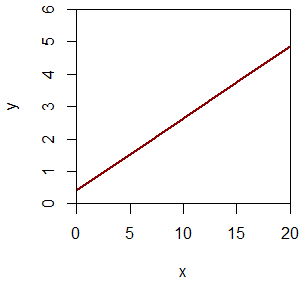
\includegraphics{./plots/plot_y_vs_x}

\end{frame}

% y = a + bx interpretation
\begin{frame}
\frametitle{Determining the slope and intercept of a line}

\center
\begin{large} \color{red} $y = a + bx$ \end{large} \color{black}: \textit{What is a? What is b?}

\vspace{-0.2cm} 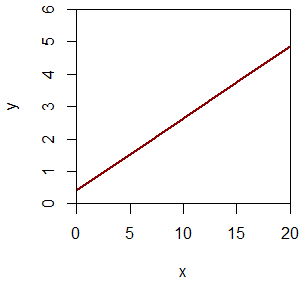
\includegraphics{./plots/plot_y_vs_x} % practice on this example, write interpretation on white board (to come back to)

\end{frame}

% FEV vs age example
\begin{frame}
\frametitle{Simple linear regression}

\center
\begin{large} \color{red} $E[Y|X] = \beta_0 + \beta_1 X$ \end{large} 

\vspace{-0.2cm} 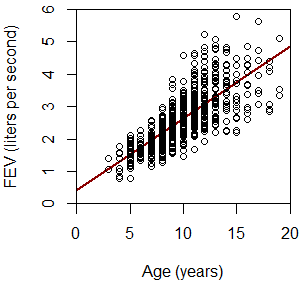
\includegraphics{./plots/plot_fev_vs_age}

\end{frame}

% what is linear regression
\begin{frame}
\frametitle{Simple linear regression}

\begin{center} 
 \color{red} $E[Y|X] = \beta_0 + \beta_1 X$ \color{black}
\end{center} \vspace{-0.3cm}

\begin{small} \textit{Let's take our data and fit the ``best" line through it. That line models the average outcome $Y$ (e.g., FEV), given the predictor $X$ (e.g., age), as a linear function of $X$ (e.g., age).} \end{small}

\center
\vspace{-0.3cm} \center 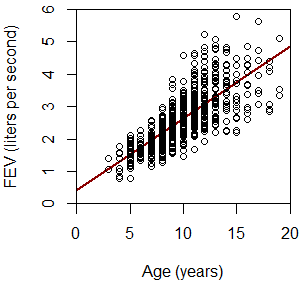
\includegraphics[height=0.65\textheight]{./plots/plot_fev_vs_age}

\end{frame}

% explain linear regression notation
\subsection{Regression Model Notation}
\begin{frame}
\frametitle{Simple linear regression: notation and terminology}
$$\color{blue} E[Y|X] \color{black} = \color{orange} \beta_0 \color{black} + \color{red} \beta_1 \color{yellow} \ X$$ \vspace{-0.6cm}

\color{blue}The average of the response, given the value of the predictor, \color{black} is \color{orange} the intercept \color{black} plus \color{red} the slope \color{black} times \color{yellow} the value of the predictor.\color{black} \pause

\vspace{-0.2cm}
\begin{itemize}
\item $Y$ = outcome, response
\item $X$ = exposure, predictor \pause
\item $E[Y] =$ expected value =  mean of $y$ in the population \pause
\item $E[Y|X]$ = conditional expectation = population mean of $Y$, given information about $X$	\pause
\item Examples: $Y$ is height, $X = 1$ if female and $0$ if male
	\begin{itemize}
	\item $E[Y]$ = 67.1" (the average height in the population)
	\item $E[Y|X = 0]$ = 69.7" (the average height of males)
	\item $E[Y|X = 1]$ = 64.6" (the average height of females)
	\end{itemize}
\end{itemize}
\end{frame}

% interpreting slope and intercept
\subsection{Interpreting Regression Coeffients}
\begin{frame}
\frametitle{Simple linear regression: interpretation}

The \textit{coefficients} ($\beta_0$,$\beta_1$) in our simple linear regression model $E[Y|X] = \beta_0 + \beta_1 X$ often have useful interpretations.

Let's start with the intercept, $\beta_0$: \textit{how would you interpret this coefficient?} \vspace{-0.3cm}
\begin{itemize}
\item[] (Hint: think about how we interpret $a$ in $y=a+bx$)\pause 
\item[] \color{blue} $\beta_0$ is the mean value of $Y$ among subjects with $X = 0$ \color{black}
\end{itemize}

And now the slope, $\beta_1$: \textit{how would you interpret this coefficient?} \vspace{-0.3cm}
\begin{itemize}
\item[] (Hint: think about how we interpret $b$ in $y=a+bx$) \pause
\item[] \color{blue} $\beta_1$ is the difference in mean value of $Y$ comparing two groups that differ in $X$ by one unit \color{black}
\end{itemize}

\end{frame}

% practice: interpreting intercepts
\begin{frame}
\frametitle{Practice: interpreting intercepts in context}

\begin{center} $E[\text{FEV} | \text{age}] = 0.43 + 0.22 \times \text{age}$ \end{center} 

\vspace{-0.3cm} Which of these is correct? \vspace{-0.3cm}
\begin{enumerate}
\item A child with age = $0$ will have FEV equal to 0.43 liters per second
\item Among all children of age 0, the average FEV is 0.43 liters per second \vspace{-0.2cm}
\end{enumerate} \pause

\color{red} Questions to consider when interpreting intercepts: \vspace{-0.3cm} \color{black}
\begin{itemize}
\item \textit{What is the scientific interpretation of ``children with age = 0``? Does our intercept make scientific sense?} \\ \pause  % Yes, age = 0 <--> birth
\item \textit{What if I replaced age with height in the formula above?} \\ \pause % No, height = 0 <-- DNE\
\item \textit{What if we did this study on adults (ages 40--60), and got the same intercept? Would you trust the intercept?} %% No! Be careful not to extrapolate too far beyond range of data
\end{itemize}

\end{frame}

% practice: interpreting slopes
\begin{frame}
\frametitle{Practice: interpreting slopes in context}

\begin{center} $E[\text{FEV} | \text{age}] = 0.43 + 0.22 \times \text{age}$ \end{center} 

\textit{What is the difference between these two interpretations?} \vspace{-0.3cm}
\begin{itemize}
\item For every one year increase in age, average FEV increases by 0.22 liters per second
\item Comparing two groups of children that differ in age by one year, the difference in average FEV will be 0.22 liters per second, with higher average FEV in the older of the two groups
\end{itemize} \pause

\textit{Which do you think is correct?} \vspace{-0.3cm} \pause 
\begin{itemize}
\item[] (Hint: this was an observational study)
\end{itemize}

% give a couple examples, some with interpretations that are ``too causal"
\end{frame}

% why do we care about the slope?
\begin{frame}
\frametitle{Why do we care about the slope?}

\begin{small} \textit{In which example(s) is there \textbf{no} association between FEV and age?} \vspace{-0.6cm} \end{small}

\hspace*{-0.6cm} 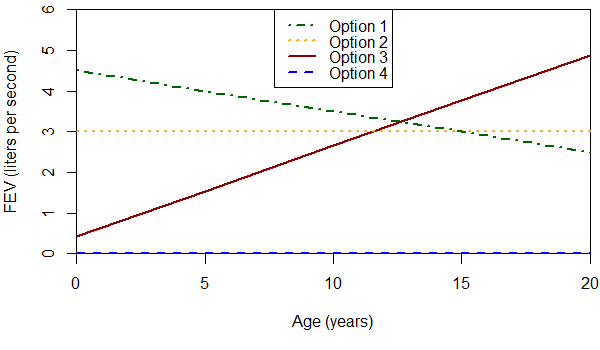
\includegraphics[width=0.9\paperwidth]{./plots/association}

\pause
 \vspace{-0.7cm} \textit{What is the slope in those cases?}
\end{frame}

\begin{frame}
\frametitle{Why do we care about the slope?}

When... \\
$\beta_1 = 0$: there is no linear association between $X$ and $Y$ \\
$\beta_1 > 0$: there is a positive linear association between $X$ and $Y$ \\
$\beta_1 < 0$: there is a negative linear association between $X$ and $Y$

\pause
Suppose we have a \textbf{scientific question:} \textit{is there an association between lung function and age?}

We can use linear regression to answer this question: \vspace{-0.3cm}
\begin{enumerate}
\item Fit the model $E[FEV|age] = \beta_0 + \beta_1 \times age$
\item Check whether or not $\beta_1 = 0$ \color{blue} (estimate, CI, p-value) \color{black}
\end{enumerate}

\pause
What \textbf{statistical question} are we answering? \textit{Is there an association between FEV and age, where association is quantified by difference in mean FEV between age groups}

\end{frame} 


% math explaining slope interpretation
\begin{frame}
\frametitle{Interpreting slopes: mathematical explanation}

For a regression model $E[Y|X] = \beta_0 + \beta_1 X$, \color{blue} we interpret the slope $\beta_1$ as the difference in mean value of $Y$ for two groups differing in $X$ by one unit. \color{black}

Why is this true?
\begin{itemize}
\item $E[Y|X = x] = \beta_0 + \beta_1 x$ \pause
\item $E[Y|X = (x+1)] = \beta_0 + \beta_1(x+1) = \beta_0 + \beta_1 x + \beta_1$ \pause
\item $E[Y|X = (x+1)] - E[Y|X = x] = \beta_1$
\end{itemize}

\end{frame}

% end of Wednesday lecture
\begin{frame}
\frametitle{What's next?}

\begin{itemize}
\item Confidence intervals and hypothesis tests for regression parameters
	\begin{itemize}
	\item \color{blue} Please read the confidence intervals analogy handout and come prepared to discuss on Friday \color{black}
	\end{itemize}
\item What it means to find the line of ``best" fit
\item Using \texttt{R} to fit linear regression models 
\end{itemize}

\end{frame}

% start of Friday lecture
\begin{frame}
\frametitle{Statistical inference: linear regression}

\color{blue} What do we know so far? \color{black}% interpreting coefficients; distinguish between truth and estimate
\begin{itemize}
\item \textbf{Estimate/statistic:} estimated regression coefficient
\item[] (After Wednesday, we know how to interpret. Today we'll talk about how to calculate.)
\end{itemize}

\color{blue} What's missing? \color{black}\pause %ask them about the 4 numbers we always want them to report
\begin{itemize}
\item \textbf{Quantifying uncertainty:} 95\% confidence interval for regression coefficient
\item \textbf{Hypothesis test:} p-value for regression coefficient \pause
\item \textit{What types of scientific questions can we answer using linear regression?}
\item \textit{How do I do all this in \texttt{R}?}
\end{itemize}

\end{frame}


% standard errors
\subsection{Confidence intervals for regression coefficents}
\begin{frame}
\frametitle{Quantifying uncertainty: standard errors (SEs)}

When we estimate regression coefficients, we also want to quantify the \color{blue} uncertainty \color{black} in these estimates.\vspace{-0.2cm} \pause

Just like we have two options for two-sample t-tests (\textit{equal} or \textit{unequal} variances), we have \color{blue} two options for calculating standard errors of regression coefficients\color{black}: \vspace{-0.3cm} \pause
\begin{itemize}
\item \textbf{Naive standard errors}: assume that the population variance of $Y$ is the same across all values of $X$ % assume homoskedasticity
	\begin{itemize}
	\item Only appropriate if this assmption is true
	\item We have no way of knowing if this assumption is true
	\end{itemize}
\item \textbf{Robust standard errors}: allow the population variance of $Y$ to differ across values of $X$ % allow for heteroskedasticity
	\begin{itemize}
	\item Appropriate if the variances differ, or if they're constant!
	\end{itemize}
\end{itemize}
\end{frame}

% picture explaining homoskedasticity vs heteroskedasticity
\begin{frame}
\frametitle{Constant vs non-constant variance}

If we sample from a population with constant variance versus non-constant variance, what does this look like?
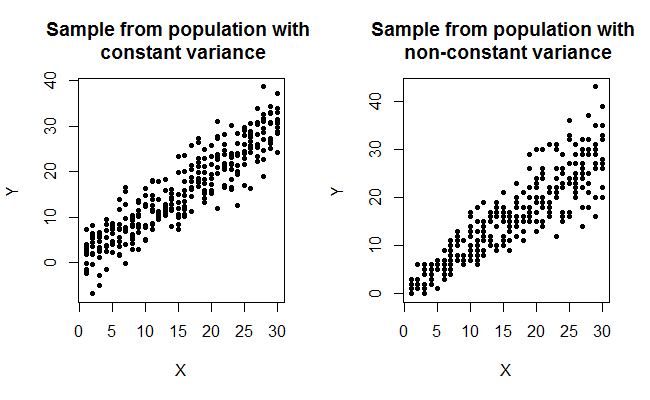
\includegraphics[width=\textwidth]{./plots/hetero}

\end{frame}

\begin{frame}
\frametitle{Choosing between naive and robust SEs}

Naive SEs assume that variance in $Y$ is constant across all values of $X$. Robust SEs are appropriate if variance is constant, or if it's non-constant!

\color{blue} Important: \color{black} what matters is whether the variance is constant \textit{in the population}, which we can't tell by looking at our data.

\color{blue} Conclusion: \color{black} unless you have a very solid scientific reason for variance being constant, use robust SEs.

\color{red} Warning: \color{black} Most software (inappropriately) uses \textit{naive} SEs, but the \texttt{uwIntroStats} package gives us \textit{robust} SEs. % they don't need to know how to calculate, just need to know where to look in regress output

\begin{footnotesize} \textit{Note: the decision about which two-sample t-test to use (equal or unequal variances) relies on a similar thought process} \end{footnotesize}
\end{frame}


% confidence intervals
\begin{frame}
\frametitle{Quantifying uncertainty: 95\% confidence intervals}

Once we have our standard error, we can calculate a 95\% confidence interval. 

Again, there are two options: \vspace{-0.3cm}
\begin{itemize}
\item $\hat{\beta} \pm 1.96 \times \widehat{SE}(\hat\beta)$
\item $\hat{\beta} \pm t_{n-2} \times \widehat{SE}(\hat\beta)$
	\begin{itemize}
	\item If $n = 10, t_{n-2} = 2.31$
	\item If $n = 100, t_{n-2} = 1.98$
	\item If $n = 1000, t_{n-2} = 1.96$
	\end{itemize}
\end{itemize}

Most software (including \texttt{uwIntroStats}) gives you the $t$-based confidence interval. When $n$ is large, there's little difference. Either way, our interpretation remains the same.

% differences between the two come from thinking about what the sampling distribution of \hat\beta is... when n is large, CLT tells us it's normal so first is good; when data are normal, \hat\beta-mu/se is t, for small or large n; in practice: t-intervals work fine in either setting because they're always wider -- may have more than 95% coverage
\end{frame}

\begin{frame}
\frametitle{Interpreting 95\% confidence intervals}

Suppose we use linear regression to evaluate the association between FEV and age, and we estimate the slope to be 0.22, with 95\% confidence interval (0.20, 0.24).

To interpret the CI for a regression coefficient: same language as CI for the mean (0.50) or difference in means (0.60, HW2)

\textit{We estimate that the difference in mean FEV comparing two groups of children that differ by one year in age is 0.22 liters per second, with higher average FEV in the older of the two groups. \color{blue} Based on a 95\% confidence interval, this estimated difference would not be judged unusual if the true difference were between 0.20 and 0.24 liters per second. \color{black}}
\end{frame}

% discussion of CI interpretation dice rolling anlogy
\begin{frame}
\frametitle{Interpreting confidence intervals: rolling the dice}

\textbf{Rolling dice}:\vspace{-0.3cm}
\begin{itemize}
\item \textit{What's random?} The process of rolling
\item Once we've rolled, there's no randomness left, and any probabilites are 0 or 1 (depending on the truth)
\end{itemize}

\pause
\textbf{Estimating quantities from data}:\vspace{-0.3cm}
\begin{itemize}
\item \textit{What's random?} The process of collecting data
\item Once we've collected data, there's no randomness left, and any probabilites are 0 or 1 (depending on the truth)
\end{itemize}

\pause
\begin{small}
Recall the definition of \textbf{probability}: the relative frequency of an event in the long run (i.e., if an experiment is repeated many times, what proportion of those times does the event occur?)\\ \pause
\color{blue} Example: \color{black} If I repeat the process of collecting data many times, and every time check if our \textit{original} confidence interval (0.20,0.24) contains the true difference in means, how often will this happen?\\ \pause \hfill \color{red} Always, or never.
\end{small}

\end{frame}

% back to road map
\begin{frame}
\frametitle{Back to our linear regression roadmap...}
\color{blue} What do we know so far? \color{black}% interpreting coefficients; distinguish between truth and estimate
\begin{itemize}
\item \textbf{Estimate/statistic:} estimated regression coefficient
\item[] (After Wednesday, we know how to interpret. Today we'll talk about how to calculate.)
\end{itemize}

\color{blue} What's missing? \color{black} %ask them about the 4 numbers we always want them to report
\begin{itemize}
\item \textbf{Quantifying uncertainty:} 95\% confidence interval for regression coefficient
\item \textbf{Hypothesis test:} p-value for regression coefficient 
\item \textit{What types of scientific questions can we answer using linear regression?}
\item \textit{How do I do all this in \texttt{R}?}
\end{itemize}
\end{frame}

\begin{frame}[noframenumbering]
\frametitle{Back to our linear regression roadmap...}
\color{blue} What do we know so far? \color{black}% interpreting coefficients; distinguish between truth and estimate
\begin{itemize}
\item \textbf{Estimate/statistic:} estimated regression coefficient
\item \textbf{Quantifying uncertainty:} 95\% confidence interval for regression coefficient
\end{itemize}

\color{blue} What's missing? \color{black} %ask them about the 4 numbers we always want them to report
\begin{itemize}
\item \textbf{Hypothesis test:} p-value for regression coefficient 
\item \textit{What types of scientific questions can we answer using linear regression?}
\item \textit{How do I do all this in \texttt{R}?}
\end{itemize}
\end{frame}

% hypothesis tests
\subsection{Hypothesis tests for regression coefficents}
\begin{frame}
\frametitle{Hypothesis tests}

$$\text{Regression Model: } E[Y|X] = \beta_0 + \beta_1 X$$

Recall that $\beta_1$ quantifies the association between $X$ and $Y$.

To test whether there is a \textit{statistically significant} association between $X$ and $Y$, \color{blue} we just need to test whether $\beta_1 = 0$: \vspace{-0.3cm} \color{black}
\begin{itemize}
\item $H_0: \beta_1 = 0$
\item $H_1: \beta_1 \not= 0$
\end{itemize}

\pause
Interpret the $p$-value just as before! (e.g., 0.59--0.60, HW2) \vspace{-0.4cm}
\begin{small}
\begin{itemize} \itemsep -2pt
\item $p < \alpha$: \textbf{reject $H_0$}, ``we have evidence to suggest that $X$ is associated with $Y$"
\item $p > \alpha$: \textbf{fail to reject $H_0$}, ``we do not have enough evidence to support the hypothesis that $X$ is associated with $Y$"
\end{itemize}
\end{small}
\end{frame}

% putting it in context: from scientific question to conclusions (FEV vs age)
\subsection{From scientific question to conclusions: continuous predictor}
\begin{frame}
\frametitle{Example: lung function and age}

\begin{enumerate}
\item \textbf{Scientific question:} is \color{blue} lung function \color{orange} associated \color{black} with age among US children? \pause
\item \textbf{Statistical question:} is there a \color{orange} difference in average \color{blue} FEV \color{black} comparing groups of US children that differ in age? \pause
	\begin{itemize}
	\item \textbf{Population:} all US children
	\item \textbf{Parameter:} population linear regression slope (diff. in means comparing groups that differ by one year in age) \pause
	\end{itemize}
\item Take a \textbf{sample} from the population: 654 children who came into a pediatric clinic for a routine check-up \pause
\item Perform \textit{statistical inference}:
	\begin{itemize}
	\item Calculate the corresponding \textbf{statistic}: sample linear regression slope (estimated difference in means comparing groups that differ by one year in age) \pause
	\item Quantify the uncertainty in your statistic
	\item Perform a hypothesis test \pause
	\end{itemize}
\item Make conclusions in context of original questions
\end{enumerate}

\end{frame}

% show R output
\begin{frame}
\frametitle{Example: lung function and age}
To fit the regression model \color{blue} $E[\text{FEV}|\text{age}] = \beta_0 + \beta_1 \text{ age}$ \color{black} in \texttt{R}:\\ (1) load \texttt{uwIntroStats}, (2) use the \texttt{regress} function. \vspace{-0.3cm}

\center
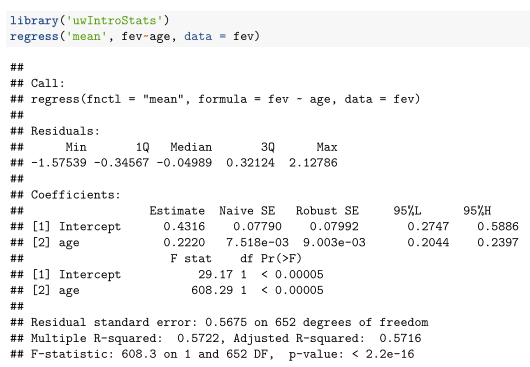
\includegraphics[width=0.55\paperwidth]{./plots/regress_fev_vs_age}
\end{frame}

% highlight what's important
\begin{frame}
\frametitle{Example: lung function and age}
Which pieces do we need to answer our question about the association between FEV and age? \vspace{-0.3cm}

\center
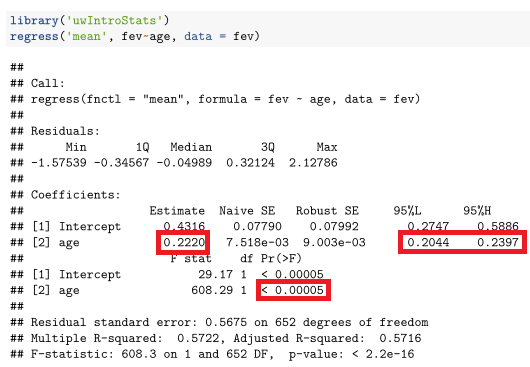
\includegraphics[width=0.55\paperwidth]{./plots/regress_fev_vs_age_highlights}
\end{frame}

% interpret results
\begin{frame}
\frametitle{Example: lung function and age}
Interpreting our results:\vspace{-0.3cm}
\begin{itemize}
\item \textit{Statistic:} We estimate that the difference in mean FEV comparing two groups of children that differ by one year in age is 0.22 liters per second, with higher average FEV in the older of the two groups. \pause
\item \textit{Uncertainty:} Based on a 95\% confidence interval, this estimated difference would not be judged unusual if the true difference were between 0.20 and 0.24 liters per second.\pause
\item \textit{Hypothesis test p-value:} These data provide strong evidence that the difference in mean FEV between groups of children that differ by one year in age is significantly different from zero (p $<$ 0.001). \pause
\item \textit{Conclusion:} These data provide evidence to suggest that older children tend to have higher FEV. 
\end{itemize}
\end{frame}

% new example: binary predictor
\begin{frame}
\frametitle{Example: lung function and age}
\textit{Why haven't we said anything about the intercept?} \pause
\begin{itemize}
\item Interpretation: We estimate that the average FEV among newborns is 0.22 L/sec \pause
\item But... 
	\begin{itemize}
	\item \textit{Is this scientifically relevant?} Maybe not.
	\item Most importantly, \color{blue} the intercept has nothing to do with our scientific question \color{black} (is FEV associated with age?) \pause
	\end{itemize}
\item Since the intercept is not relevant to our primary scientific question, we don't care about the CI or p-value
\end{itemize}
\end{frame}


% putting it in context: from scientific question to conclusions (FEV vs sex) = special case with binary predictor
%%%% if time: use genetics example instead
\subsection{From scientific question to conclusions: binary predictor}
\begin{frame}
\frametitle{Example: lung function and sex}

\begin{enumerate}
\item \textbf{Scientific question:} do boys and girls (in the US) have different lung function?
\item \textbf{Statistical question:} is there a difference in average FEV between boys and girls in the US?
\end{enumerate} 

Earlier this week, we used the two-sample t-test (with unequal variances) to address this question.

We can also use linear regression!
\end{frame}

% show R output
\begin{frame}
\frametitle{Example: lung function and sex}
To fit the regression model \color{blue} $E[\text{FEV}|\text{male}] = \beta_0 + \beta_1 \text{ male}$ \color{black} in \texttt{R}:\\ (1) load \texttt{uwIntroStats} (not shown here), (2) re-code \texttt{sex} to create a binary variable \texttt{male}, and (3) run \texttt{regress}. \vspace{-0.5cm}

\center
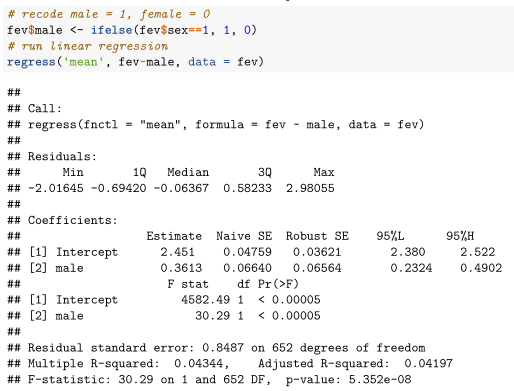
\includegraphics[width=0.6\paperwidth]{./plots/regress_fev_vs_sex}

\end{frame}

\begin{frame}
\frametitle{Example: lung function and sex}

Our linear regression results:

\begin{itemize}
\item \textit{Statistic:} We estimate that the difference in mean FEV between girls and boys is 0.361 liters per second (with boys tending to have the higher mean FEV). \pause
\item \textit{Uncertainty:} Based on a 95\% confidence interval, this observed difference would not be judged unusual if the true difference were between 0.232 and 0.490 liters per second.\pause
\item \textit{Hypothesis test p-value:} These data provide strong evidence that the difference in mean FEV between groups is different from zero (p $<$ 0.001).\pause
\item \textit{Conclusion:} These data provide evidence to suggest that male children tend to have higher FEV.
\end{itemize}

\end{frame}

\begin{frame}
\frametitle{Example: lung function and sex}

Our t-test results: 

\begin{itemize}
\item \textit{Statistic:} We estimate that the difference in mean FEV between girls and boys is 0.361 liters per second (with boys tending to have the higher mean FEV). 
\item \textit{Uncertainty:} Based on a 95\% confidence interval, this observed difference would not be judged unusual if the true difference were between 0.232 and 0.490 liters per second.
\item \textit{Hypothesis test p-value:} These data provide strong evidence that the difference in mean FEV between groups is different from zero (p $<$ 0.001).
\item \textit{Conclusion:} These data provide evidence to suggest that sex is associated with FEV in children.
\end{itemize}

\end{frame}

\begin{frame}
\frametitle{Example: lung function and sex}

\begin{itemize}
\item \color{blue} If you use linear regression with a binary predictor, this is essentially the same as performing a two-sample t-test \color{black}
	\begin{itemize}
	\item Difference in mean between groups differing by one unit (for a binary predictor, you can only differ by one unit)
	\end{itemize}
\item If you use naive SEs, this is \textit{exactly} equivalent to the t-test which presumes equal variances
\item If you use robust SEs, this is \textit{approximately} equivalent\footnote[frame]{Our results look exactly the same, but if you go out to more digits you see slight differences in, e.g., the CI: (0.23235, 0.49020) and (0.23238, 0.49017) for the t-test and linear regression, respectively\\} to the t-test which allows for unequal variances
\end{itemize}

\vspace{-0.2cm} No matter your choice of SEs, your estimates will be the same: $\beta_1$ = the differences in means, $\beta_0 = $ the mean in ``group 0"


\end{frame}

% "Under the hood" -- how do we get a linear regression line?
%%% explain ideas behind least squares estimation
\subsection{Under the hood: least squares estimation}
\begin{frame}
\frametitle{Least squares estimation}
What is \texttt{R} doing \textit{under the hood} to get these regression coefficient estimates?\vspace{-0.6cm} \pause 

\center 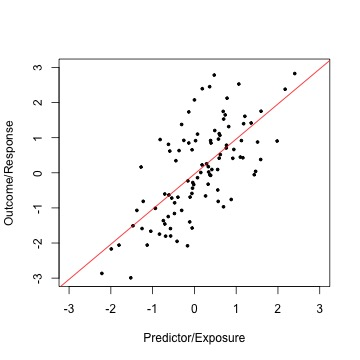
\includegraphics[height=0.7\textheight]{./plots/linear-regr}
\end{frame}

\begin{frame}
\frametitle{Least squares estimation}
\textit{Least squares:} minimize the sum of the squared distances from the observed points to the fitted line.\vspace{-0.6cm}

\center 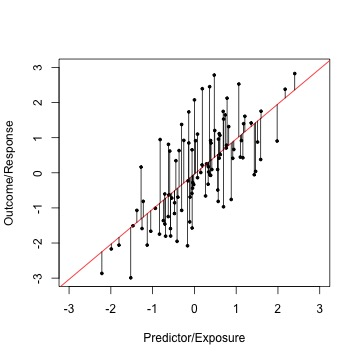
\includegraphics[height=0.7\textheight]{./plots/linear-regr-ls}
\end{frame}

\begin{frame}
\frametitle{Least squares estimation: technical details}
\textit{Least squares:} minimize the sum of the squared distances from the observed points to the fitted line. \pause

We can write this as an optimization problem, $$ \text{argmin}_{\beta_0,\beta_1} \sum_{i=1}^n \left(Y_i - \left[\beta_0 + \beta_1 X_i\right]\right)^2,$$ \pause which has a closed form solution:\vspace{-0.3cm}
\begin{itemize}
\item $\hat\beta_1 = \frac{\sum_i \left(X_i - \bar{X}\right)\left(Y_i - \bar{Y}\right)}{\sum_i \left(X_i - \bar{X}\right)^2}$
\item $\hat\beta_0 =\bar{Y} - \hat\beta_1 \bar{X}$
\end{itemize}

\center \color{blue} \textit{You will \textbf{NOT} be tested on these!} \color{black}
\end{frame}

\subsection{Regression and correlation}
% aside: connect to correlation
\begin{frame}
\frametitle{Simple linear regression and correlation}

Notice how much our slope estimate looks like Pearson's correlation ($r$): 
$$\hat\beta_1 = \frac{\sum_i \left(X_i - \bar{X}\right)\left(Y_i - \bar{Y}\right)}{\sum_i \left(X_i - \bar{X}\right)^2}$$
$$r = \frac{\sum_i \left(X_i - \bar{X}\right)\left(Y_i - \bar{Y}\right)}{\sqrt{\sum_i\left(X_i - \bar{X}\right)^2} \sqrt{\sum_i \left(Y_i - \bar{Y}\right)^2}}$$ \pause

\begin{itemize}\vspace{-0.3cm}
\item $\hat\beta_1$ and $r$ have the same sign: both positive, both negative, or both zero
\item Testing $H_0: r = 0$ is equivalent to testing $H_0: \beta_1 = 0$
\item $\hat\beta_1$ has a more meaningful (and scientifically relevant) interpretation
\item (Coming soon:) Linear regression also lets us adjust for other variables; correlation does not
\end{itemize}

\end{frame}


\begin{frame}
\frametitle{Index Card \# 3}

\begin{enumerate}
\item Name
\item Something you learned this week.
\item Something you \textit{were} struggling with/had questions about, but now feel more confident about.
\item Something you \textit{are} struggling with/have questions about.
\item Does our office hours time (Wed, 2--4) work for you?
\item Have you ever used Poll Everywhere?
\end{enumerate}

\end{frame}

%% start here 4/9
\begin{frame}
\frametitle{Linear regression roadmap}
\color{blue} What do we know so far? \color{black}\vspace{-0.3cm}% interpreting coefficients; distinguish between truth and estimate
\begin{itemize}
\item \textbf{Estimate/statistic:} estimated regression coefficient
\item \textbf{Quantifying uncertainty:} 95\% confidence interval for regression coefficient
\item \textbf{Hypothesis test:} p-value for regression coefficient 
\item \textit{What types of scientific questions can we answer using linear regression?}
	\begin{itemize}
	\item Continuous outcome vs continuous predictor
	\item Continuous outcome vs binary predictor
	\end{itemize}
\item \textit{How do I do all this in R?} (and what R is doing)
\end{itemize}

\color{blue} What's next?\vspace{-0.3cm}
\begin{itemize}
\item Transforming our predictor or outcome
\item Linear regression with a categorical predictor
\end{itemize}
\end{frame}

\subsection{Transformations}
% Warm-up activity: FEV vs age
\begin{frame}
\frametitle{Interpreting coefficients (no transformation)}
How do we interpret $\beta_0, \beta_1$ in this linear regression model? $$E[\text{FEV}|\text{Age}] = \beta_0 + \beta_1 \text{Age}$$

$\beta_0$: average value of $Y$ among subjects with $X = 0$ \\ \pause
\ \ \ \ \ \color{blue} average FEV (l/sec) among newborns \color{black} \pause

$\beta_1$: difference in average value of $Y$ comparing two groups that differ in $X$ by one unit\\ \pause
\ \ \ \ \ \color{blue} difference in average FEV (l/sec) comparing two groups that differ in age by one year 
\end{frame}

% Warm-up activity: Age+3
\begin{frame}
\frametitle{Interpreting coefficients after a transformation}
How do we interpret $\beta_0$ in this linear regression model? $$E[\text{FEV}|\color{blue}(\text{Age}-3)\color{black}] = \beta_0 + \beta_1 \color{blue}\left(\text{Age}-3\right)\color{black}$$

\vspace{-0.5cm}
$\beta_0$: average value of $Y$ among subjects with $X = 0$ \\ \pause
\ \ \ \ \ average FEV (l/sec) among kids with $\text{Age} -3 = 0$\\ \pause
\ \ \ \ \ \color{blue} average FEV (l/sec) among 3 year olds \color{black} \pause

Why are those last two interpretations equivalent?
\begin{align*}
(\text{Age}-3) &= 0 \\ 
\text{Age} &= 3
\end{align*}
\end{frame}

% Age-3: slope
\begin{frame}
\frametitle{Interpreting coefficients after a transformation}
How do we interpret $\beta_1$ in this linear regression model? $$E[\text{FEV}|(\text{Age}-3)] = \beta_0 + \beta_1 \left(\text{Age}-3\right)$$

\vspace{-0.5cm}
$\beta_1$: difference in average value of $Y$ comparing two groups that differ in $X$ by one unit\\ \pause
\ \ \ \ \ difference in average FEV (l/sec) comparing two groups that differ in $\text{Age}-3$ by one year\\ \pause
\ \ \ \ \ \color{blue} difference in average FEV (l/sec) comparing two groups that differ in age by one year \color{black}\pause

Why are those last two interpretations equivalent?
\begin{align*}
(\text{Age}-3) = x+1 &\color{red} \text{ vs } \color{black} (\text{Age}-3) = x \\
\text{Age} = x+4 &\color{red} \text{ vs } \color{black} \text{Age} = x+3
\end{align*}
\end{frame}

% Warm-up activity
\begin{frame}
\frametitle{Interpreting coefficients: your turn!}
On a piece of paper, please:\vspace{-0.3cm}
\begin{enumerate} \itemsep +5pt
\item Write your name
\item Interpret\footnote[frame]{\color{blue} Don't forget units! FEV = liters/second, Age = years} $\beta_0, \beta_1$ in the following models:
	\begin{enumerate}\itemsep +5pt
	\item $E[\text{FEV}|\left(\text{Age}-\overline{Age}\right)] = \beta_0 + \beta_1 \left(\text{Age}-\overline{Age}\right)$ 
	\item $E[\text{FEV}|\left(\frac{\text{Age}}{10}\right)] = \beta_0 + \beta_1 \left(\frac{\text{Age}}{10}\right)$ 
	\item $E[\text{FEV}|\left(\frac{\text{Age}-3}{10}\right)] = \beta_0 + \beta_1 \left(\frac{\text{Age}-3}{10}\right)$ 
	\end{enumerate}
\item Interpret $\beta_0, \beta_1$ in the following models:
	\begin{enumerate}\itemsep +5pt
	\item $E[(\text{FEV}\times 60)|\text{Age}] = \beta_0 + \beta_1 \text{Age}$ 
	\item $E[\left(\frac{\text{FEV}}{3.78541}\right)|\text{Age}] = \beta_0 + \beta_1 \text{Age}$ \begin{scriptsize}\\(Hint: 1 gallon = 3.78541 liters)\end{scriptsize}
	\end{enumerate}
\end{enumerate}
\end{frame}

% pause to walk through answers

% motivation for linear transformations
\subsubsection{Linear transformations}
\begin{frame}
\frametitle{Linear transformations of $X$ and $Y$}

\textit{Linear transformations:} adding, subtracting, multiplying, and/or dividing by some constant

Which transformations changed our interpretation of $\beta_0$?\vspace{-0.3cm}\pause
\begin{itemize}
\item[] Adding (subtracting) a constant to (from) $X$
\item[] Any change to $Y$\pause
\end{itemize}

Which transformations changed our interpretation of $\beta_1$?\pause
\vspace{-0.3cm}
\begin{itemize}
\item[] Dividing (multiplying) $X$ by a constant  
\item[] Any change to $Y$
\end{itemize}
\end{frame}

\begin{frame}
\frametitle{Why transform $X$ and/or $Y$?}
Why might we want to transform our variables? 
\begin{itemize}
\item \textit{Make interpretation of $\beta_0$ more scientifically meaningful} (e.g., so we're not talking about the average FEV among people with height 0")
\item \textit{Make estimate of $\beta_0$ more trustworhty} (e.g., so we're not estimating the average FEV among newborns if all our data were collected on senior citizens)
\item \textit{Change units of outcome and/or predictor} (e.g., difference in FEV in liters/minute comparing two groups that differ in age by one year)
\end{itemize}

We'll come back to this...
\end{frame}

% summary of types of transformations they should know
\begin{frame}
\frametitle{Types of transformations}

So far we've seen:
\begin{enumerate}
\item Adding/subtracting a constant (e.g., $\text{Age} - \overline{Age}$)
\item Multiplying/dividing by a constant (e.g., $\text{Age}/10$)
\item A combination of 1. and 2. (e.g., $(\text{Age}-3)/10$)
\end{enumerate}

What other types of transformations might we use?
\begin{enumerate}
\item Log transformations
\item Polynomial transformations (e.g., $x + x^2$)
\end{enumerate}

\end{frame}

\subsubsection{Log transformations}
% log(X) - beta_0
\begin{frame}
\frametitle{Transformations: $\log(X)$}
\begin{center} $E[FEV|\log(\text{Height})] = \beta_0 + \beta_1 \log(\text{Height})$ \end{center}

$\beta_0$: average value of $Y$ among subjects with $X = 0$\\ \pause 
\ \ \ \ \ average FEV among subjects with $\log(\text{Height}) = 0$\\ \pause 
\ \ \ \ \ \color{blue} average FEV among subjects who are 1 inch tall \color{black}  \pause

Why are those last two interpretations equivalent?
\begin{align*}
\log(\text{Height}) & = 0 \\
e^{\log(\text{Height})} & = e^0 \\
\text{Height} & = 1\\
\end{align*}
\begin{footnotesize} Note: in statistics (and in \texttt{R}), when we write $\log$, we mean $\log_e = \ln$ \end{footnotesize}
\end{frame}

% log(X) - beta_1
\begin{frame}
\frametitle{Transformations: $\log(X)$}
\begin{center} $E[FEV|\log(\text{Height})] = \beta_0 + \beta_1 \log(\text{Height})$ \end{center}

$\beta_1$: difference in average value of $Y$ comparing two groups that differ in $X$ by one unit\\ \pause
\ \ \ \ \ difference in average FEV comparing two groups that differ in $\log(\text{Height})$ by one unit\\ \pause
\ \ \ \ \ \color{blue} difference in average FEV comparing two groups that differ in height by a multiplicative factor of $e$ (2.718...) \color{black} \pause

Why are those last two interpretations equivalent?
\begin{align*}
\log(\text{Height}) = x + 1 &\color{red}\text{ vs }\color{black} \log(\text{Height}) = x \\
e^{\log(\text{Height})} = e^{x+1} &\color{red}\text{ vs }\color{black} e^{\log(\text{Height})} = e^x \\
\text{Height} = e^{x}e &\color{red}\text{ vs }\color{black} \text{Height} = e^{x}
\end{align*}
\end{frame}

% log(X) - beta_1
\begin{frame}
\frametitle{Transformations: $\log(X)$}
An $e$-fold difference between two groups is not very intuitive. How can we make our interpretation of $\beta_1$ better?

Option 1: use a different base\pause
\begin{itemize}
\item $E[FEV|\color{blue}\log_2\color{black}(Height)] = \beta_0 + \beta_1 \color{blue}\log_2\color{black}(Height)$
	\begin{itemize}
	\item $\beta_0$: average FEV among subjects who are 1" tall
	\item $\beta_1$: difference in average FEV comparing groups that differ in height by a \color{blue} multiplicative factor of 2\color{black}
	\end{itemize} \pause
\item $E[FEV|\color{blue}\log_{10}\color{black}(Height)] = \beta_0 + \beta_1 \color{blue}\log_{10}\color{black}(Height)$
	\begin{itemize}
	\item $\beta_0$: average FEV among subjects who are 1" tall
	\item $\beta_1$: difference in average FEV comparing groups that differ in height by a \color{blue}multiplicative factor of 10\color{black}
	\end{itemize}
\end{itemize}
\end{frame}

% log(X) - beta_1
\begin{frame}
\frametitle{Transformations: $\log(X)$}
An $e$-fold difference between two groups is not very intuitive. How can we make our interpretation of $\beta_1$ better?

Option 2: fit the same model \begin{scriptsize}($E[FEV|\log(Height)] = \beta_0 + \beta_1\log(Height)$)\end{scriptsize} but interpret $c \times \beta_1$ rather than $\beta_1$ \pause

\textit{Example:} $\color{blue}\log(1.1)\color{black}\beta_1$ is the difference in average FEV comparing two groups that differ in height by a \color{blue}multiplicative factor of 1.1 \color{black} (i.e., a 10\% difference)\pause
	\begin{align*}
	E[FEV|&\log(Height=1.1x)]-E[FEV|\log(Height=x)] \\
	& = \left[\beta_0 + \beta_1\log(1.1x)\right] - \left[\beta_0 + \beta_1 \log(x) \right]\\
	& = \left[\beta_0 + \beta_1\{\log(1.1)+\log(x)\}\right] - \left[\beta_0 + \beta_1 \log(x) \right]\\
	& = \left[\beta_0 + \beta_1\log(1.1)+\beta_1\log(x)\right]-\left[\beta_0 + \beta_1 \log(x) \right]\\
	& = \beta_1\log(1.1)
	\end{align*}
\end{frame}

% summary: log(X)
\begin{frame}
\frametitle{Transformations: $\log(X)$}
Tying it all together...
\begin{itemize}
\item \color{blue} Regression model: \color{black} $E[Y|\log(X)] = \beta_0 + \beta_1\log(X)$
\item \color{blue} $\beta_0$: \color{black} average value of $Y$ among subjects with $X = 1$
\item \color{blue} $\log(k)\times\beta_1$: \color{black} difference in average value of $Y$ comparing two groups that differ in $X$ by a multiplicative factor of $k$
\end{itemize}\pause

Why would we want to do this type of transformation?
\begin{itemize}
\item Sometimes it is more scientifically relevant to talk about multiplicative changes in $X$ rather than differences in $X$
\item Types of variables that we often $\log$ transform:
	\begin{itemize}
	\item Money (e.g., salary, home prices)
	\item Biological measurements (e.g., prostate specific antigen in prostate cancer, serum creatinine in kidney disease)
	\end{itemize}
\end{itemize}
\end{frame}

% log(Y)
\begin{frame}
\frametitle{Transformations: $\log(Y)$}
\begin{center} $E[\log(FEV)|Height] = \beta_0 + \beta_1 Height$ \end{center}
$\beta_0$: average value of $Y$ among subjects with $X = 0$\\ \pause
\ \ \ \ \ average $\log(FEV)$ among subjects that are 0" tall \\ \pause
\ \ \ \ \ log geometric mean FEV among subjects that are 0" tall \\ 
\color{blue} $e^{\beta_0}$: geometric mean of FEV among subjects that are 0" tall \color{black}\pause

Why are those interpretations equivalent?\vspace{-0.3cm}
\begin{itemize}
\item[] \textit{Arithmetic mean}: $\frac{1}{n} \sum_{i=1}^n a_i$
\item[] \textit{Geometric mean}: $\left(\prod_{i=1}^n a_i\right)^{\frac{1}{n}} = e^{\frac{1}{n} \sum_{i=1}^n \log(a_i)}$
\end{itemize}
\vspace{-0.3cm}
\begin{center} \begin{footnotesize}The \color{blue} ``average of $\log(Y)$" \color{black} = $\frac{1}{n}\sum \log(Y_i)$ \ \color{blue} \textit{is the same as} \color{black}\\the \color{blue}``log of the geometric mean of $Y$" \color{black}= $\log(e^{\frac{1}{n}\sum \log(Y_i)} = \frac{1}{n}\sum \log(Y_i)$.\end{footnotesize}\end{center}
\end{frame}

%log(Y) - beta_1
\begin{frame}
\frametitle{Transformations: $\log(Y)$}
\begin{center} $E[\log(FEV)|Height] = \beta_0 + \beta_1 Height$ \end{center}
$\beta_1$: difference in average values of $Y$ comparing two groups that differ in $X$ by one unit\\ \pause
\ \ \ \ \ difference in average $\log(FEV)$ comparing two ...\\ \pause
\ \ \ \ \ difference in log geometric mean FEV comparing two ... \\ 
\color{blue} $e^{\beta_1}$: ratio of geometric mean FEV comparing two ... \color{black} \pause

Why are those interpretations equivalent?\vspace{-0.3cm}
\begin{align*}
\beta_1 & = \log(\text{GM}[Y|X=x+1])-\log(\text{GM}[Y|X=x])\\
& = \log\left(\text{GM}[Y|X=x+1]\div\text{GM}[Y|X=x]\right)\\
e^{\beta_1} & = \text{GM}[Y|X=x+1]\div\text{GM}[Y|X=x]
\end{align*}
\end{frame}

% summary: log(Y)
\begin{frame}
\frametitle{Transformations: $\log(Y)$}
Tying it all together...
\begin{itemize}
\item \color{blue} Regression model: \color{black} $E[\log(Y)|X] = \beta_0 + \beta_1X$
\item \color{blue} $e^{\beta_0}$: \color{black} geometric mean of $Y$ among subjects with $X = 0$
\item \color{blue} $e^{\beta_1}$: \color{black} ratio of geometric means of $Y$ comparing two groups that differ in $X$ by one unit
\end{itemize}\pause

Why would we want to do this type of transformation?\vspace{-0.3cm}
\begin{itemize}
\item Sometimes it is more scientifically relevant to talk about multiplicative changes in $Y$ rather than differences
\item Types of variables that we often $\log$ transform:
	\begin{itemize}
	\item Money (e.g., salary, home prices)
	\item Biological measurements (e.g., prostate specific antigen in prostate cancer, serum creatinine in kidney disease)
	\end{itemize}
\end{itemize}
\end{frame}

% summary: log(Y)
\begin{frame}
\frametitle{Transformations: $\log(Y)$ \textit{and} $\log(X)$}
\center What if we log-transformed our outcome \textit{and} our predictor? % probably skip
\end{frame}

\subsubsection{Polynomial transformations}
% polynomial
\begin{frame}
\frametitle{Transformations: polynomial}
\begin{center} $E[\text{FEV}| \text{Height}] = \beta_0 + \beta_1 \text{Height} + \beta_2 \text{Height}^2$ \end{center}

Now we have three coefficients: $\beta_0, \beta_1, \beta_2$\pause

\color{blue} $\beta_0$: average FEV among subjects who are 0" tall \color{black} \pause
\begin{align*}
E[\text{FEV}|\text{Height} = 0] & = \beta_0 + \beta_1 (0) + \beta_2(0)^2 \\
& = \beta_0 + 0 + 0 \\
& = \beta_0
\end{align*}
\end{frame}

% poly - slope
\begin{frame}
\frametitle{Transformations: polynomial}
\begin{center} $E[\text{FEV}| \text{Height}] = \beta_0 + \beta_1 \text{Height} + \beta_2 \text{Height}^2$ \end{center}

$\beta_1$: \color{red} NOT \color{black} the difference in average FEV comparing groups of subjects that differ in height by one inch\pause
\begin{align*}
E[&\text{FEV}|\text{Height} = x+1] -E[\text{FEV}|\text{Height} = x]\\
& = \left[\beta_0 + \beta_1 (x+1) + \beta_2(x+1)^2\right] -\left[\beta_0 + \beta_1 (x) + \beta_2(x)^2\right]\\
& = \beta_1 + \beta_2(2x+1) \\
\end{align*}\pause
\color{blue} $\beta_1,\beta_2$: no straightforward interpretation \color{black}
\end{frame}

\begin{frame}
\frametitle{Transformations: polynomial}
Tying it all together...
\begin{itemize}
\item \color{blue} Regression model: \color{black} $E[Y|X] = \beta_0 + \beta_1X + \beta_2 X^2 + \cdots$
\item \color{blue} $\beta_0$: \color{black} average value of $Y$ when $X = 0$
\item \color{blue} $\beta_1, \beta_2, \cdots$: \color{black} no straightforward interpretation
\end{itemize}\pause

Why would we want to do this type of transformation?
\begin{itemize}
\item Sometimes we might have scientific reason to believe that $Y$ is related to $X^2$ (e.g., area) or $X^3$, rather than just $X$
\item Model non-linearity in the relationship between $X$ and $Y$
	\begin{itemize}
	\item Important for prediction
	\item Not necessary for showing associations 
	\end{itemize}
\end{itemize}\pause

Alternative: $E[\log(Y)|\log(X)] = \beta_0 + \beta_1 \log(X)$

\end{frame}

\begin{frame}
\frametitle{Summary: why transform $X$ and/or $Y$?}
Why might we want to transform our variables? \vspace{-0.3cm}
\begin{itemize}
\item Scientific motivation
	\begin{itemize}
	\item Improve interpretation
	\item More realistically model the relationships we think exist between variables
		\begin{itemize}
		\item Multiplicative (ratio) vs additive (difference)
		\item Geometric mean vs arithmetic mean
		\end{itemize}
	\end{itemize}
\item Account for non-linearity 
	\begin{itemize}
	\item Important for prediction
	\item Not necessarily for detecting associations
	\end{itemize}
\end{itemize}

\color{red} Important: \color{black} decision to transform should always be made \textit{before} looking at your data, on the basis of \textit{scientific motivations}
\end{frame}


\subsection{Categorical predictor}
% dummy variables
\begin{frame}
\frametitle{Linear regression with a categorical predictor}

What if our scientific question is about the association between a continuous outcome and a categorical predictor?\pause

If the predictor is binary (e.g., smoker):\vspace{-0.3cm}
\begin{itemize}
\item Re-code as 0/1 
\end{itemize}\pause

If the predictor is ordinal (e.g., genotype = AA, Aa, aa): \vspace{-0.3cm}
\begin{itemize}
\item You \textit{might} be able to find a meaningful way to represent numerically (e.g., number of A alleles: 2, 1, 0)
\item Often not possible to do this re-coding
\end{itemize}\pause

If the predictor is nominal (e.g., ancestry = Afr, NAm, Eur):\vspace{-0.3cm}
\begin{itemize}
\item No meaningful numeric representation
\end{itemize}
\end{frame}

\begin{frame}
\frametitle{Linear regression with a categorical predictor}
What can we do? \pause We use \textit{dummy variables}...
$$E[\text{Systolic Blood Pressure}|\text{Ancestry}] = \beta_0 + \beta_1 \text{African} + \beta_2 \text{European}$$

\vspace{-0.5cm}
\begin{itemize}
\item \textit{African} = 1 if \textit{Ancestry} = \textit{African}, and 0 otherwise
\item \textit{European} = 1 if \textit{Ancestry} = \textit{European}, and 0 otherwise
\end{itemize}\pause

$\beta_0$: average SBP among subjects with \textit{Native American} ancestry
\begin{align*}
E[\text{SBP}|\text{Ancestry} = NAm] &= \beta_0 + \beta_1(0) + \beta_2(0) \\
& = \beta_0
\end{align*}
\end{frame}

% dummy - beta1
\begin{frame}
\frametitle{Linear regression with a categorical predictor}
What can we do? We use \textit{dummy variables}...
$$E[\text{Systolic Blood Pressure}|\text{Ancestry}] = \beta_0 + \beta_1 \text{African} + \beta_2 \text{European}$$

\vspace{-0.5cm}
\begin{itemize}
\item \textit{African} = 1 if \textit{Ancestry} = \textit{African}, and 0 otherwise
\item \textit{European} = 1 if \textit{Ancestry} = \textit{European}, and 0 otherwise
\end{itemize}

$\beta_1$: difference in average SBP between groups with Native American and African ancestry
\begin{align*}
E[&\text{SBP}|\text{Ancestry} = Afr] - E[\text{SBP}|\text{Ancestry} = NAm] \\
&= \left[\beta_0 + \beta_1(1) + \beta_2(0)\right] - \left[\beta_0 + \beta_1(0) + \beta_2(0) \right] \\
& = \beta_1
\end{align*}
\end{frame}

% dummy - beta2
\begin{frame}
\frametitle{Linear regression with a categorical predictor}
What can we do? We use \textit{dummy variables}...
$$E[\text{Systolic Blood Pressure}|\text{Ancestry}] = \beta_0 + \beta_1 \text{African} + \beta_2 \text{European}$$

\vspace{-0.5cm}
\begin{itemize}
\item \textit{African} = 1 if \textit{Ancestry} = \textit{African}, and 0 otherwise
\item \textit{European} = 1 if \textit{Ancestry} = \textit{European}, and 0 otherwise
\end{itemize}

$\beta_2$: difference in average BP between groups with Native American and European ancestry
\begin{align*}
E[&\text{SBP}|\text{Ancestry} = Eur] - E[\text{SBP}|\text{Ancestry} = NAm] \\
&= \left[\beta_0 + \beta_1(0) + \beta_2(1)\right] - \left[\beta_0 + \beta_1(0) + \beta_2(0) \right] \\
& = \beta_2
\end{align*}
\end{frame}

\begin{frame}
\frametitle{Linear regression with a categorical predictor}
$$E[\text{Systolic Blood Pressure}|\text{Ancestry}] = \beta_0 + \beta_1 \text{African} + \beta_2 \text{European}$$

\vspace{-0.3cm}
\begin{itemize}
\item If we have $k$ categories, we create $k-1$ \textit{dummy variables} (and the $k$th category is captured in the intercept)
\item \texttt{R} can automatically set these up for you :
\item[] \texttt{regress('mean', sbp $\sim$ factor(ancestry), data = bloodpressure)}
\item If we want to test whether SBP is associated with ancestry, we need to test if \textit{both} $\beta_1 = 0, \beta_2 = 0$
\end{itemize}

This is a preview of \textit{multiple linear regression}!

\end{frame}

\section{Multiple Linear Regression}
\begin{frame}
\frametitle{SECTION 2: MULTIPLE LINEAR REGRESSION}
By the end of Section 2, you should be able to: \vspace{-0.4cm}
\begin{itemize}
\item Identify potential variables that \textcolor{red}{confound} the association between the predictor of interest and the outcome, and
\item describe \textbf{why} you will adjust for these variables in a regression analysis.
\item Identify potential variables that \textcolor{blue}{modify} the association between the predictor of interest and the outcome, and  
\item describe \textbf{how} you will test for  differential effects.
\item Identify potential variables that help \textcolor{green}{reduce the variability} of our estimates.
\item \textbf{Interpret} parameters in a multiple linear regression model.
\item \textbf{Fit} multiple linear regression models in \texttt{R}, and
\item \textbf{interpret} the output to perform hypothesis tests.
\end{itemize}

\end{frame}

\subsection{Motivation}
\begin{frame}
\frametitle{Multiple regression: motivation}

So far, we have considered the relationship between the outcome, $Y$, and a \textcolor{green}{single} predictor of interest, $X$.

However, there may be other variables that influence the association between our predictor of interest and the outcome, by:
\begin{itemize}
\item \textcolor{red}{confounding} the association 
\item \textcolor{blue}{modifying} the association
\item providing information that \textcolor{green}{reduces the variability} of our estimates
\end{itemize} 
\end{frame}

% confounding
\begin{frame}
\frametitle{Multiple regression: motivation}
What do you think the relationship is between $X_1$ and $Y$?

\vspace{-0.3cm}
\centering
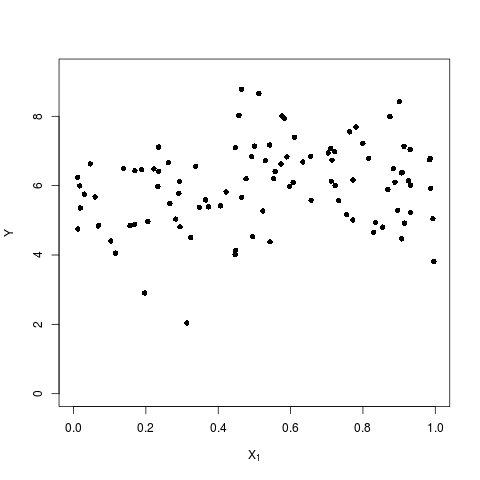
\includegraphics[width = 0.75\textwidth]{./plots/confounding_simple.png}
\end{frame}

\begin{frame}
\frametitle{Multiple regression: motivation}
What do you think the relationship is between $X_1$ and $Y$?

\vspace{-0.3cm}

\centering
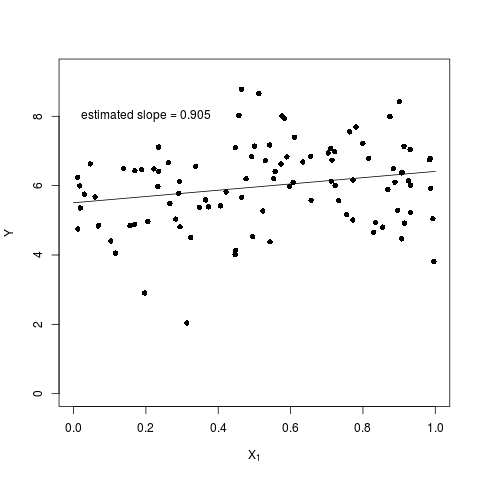
\includegraphics[width = 0.75\textwidth]{./plots/confounding_simple_with_line.png}
\end{frame}

\begin{frame}
\frametitle{Multiple regression: motivation}
How about now?

\vspace{-0.3cm}
\centering
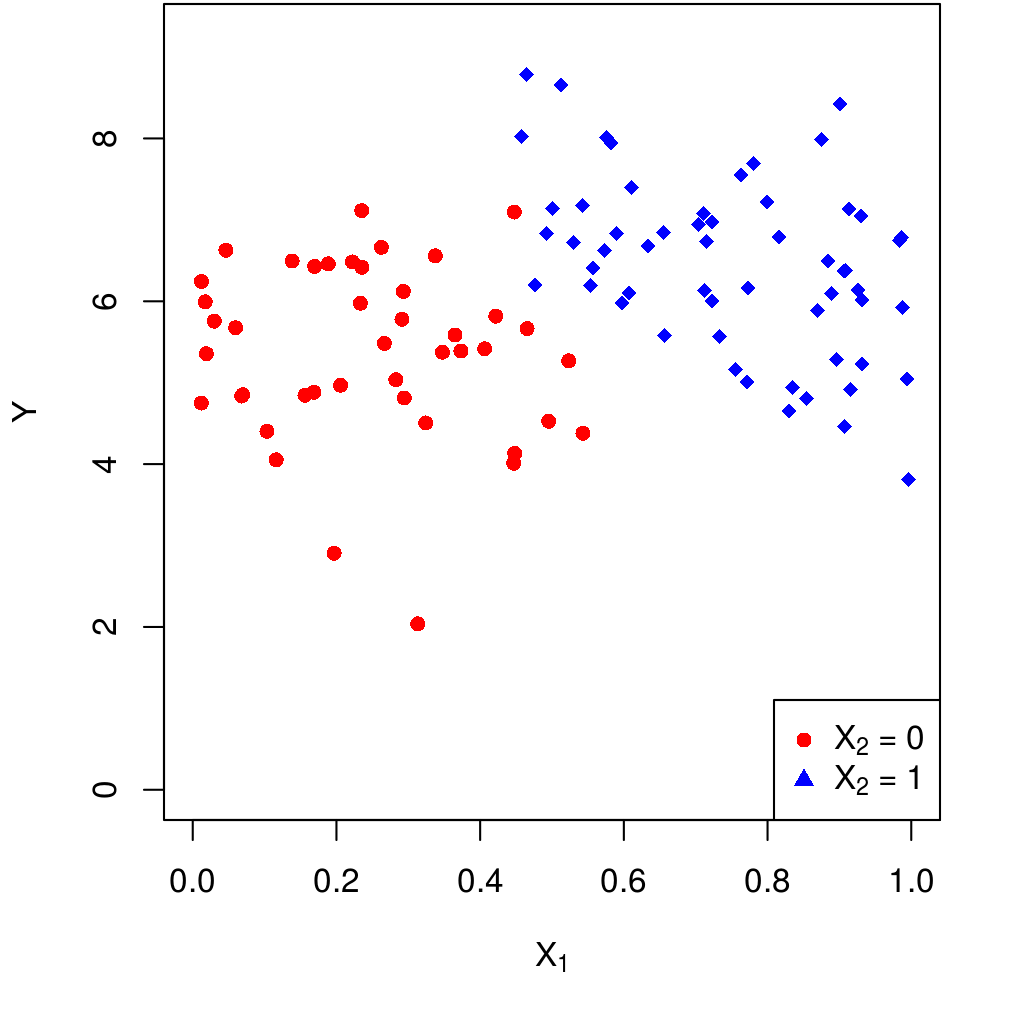
\includegraphics[width = 0.75\textwidth]{./plots/confounding_colored.png}
\end{frame}

\begin{frame}
\frametitle{Multiple regression: motivation}
How about now?

\vspace{-0.3cm}
\centering
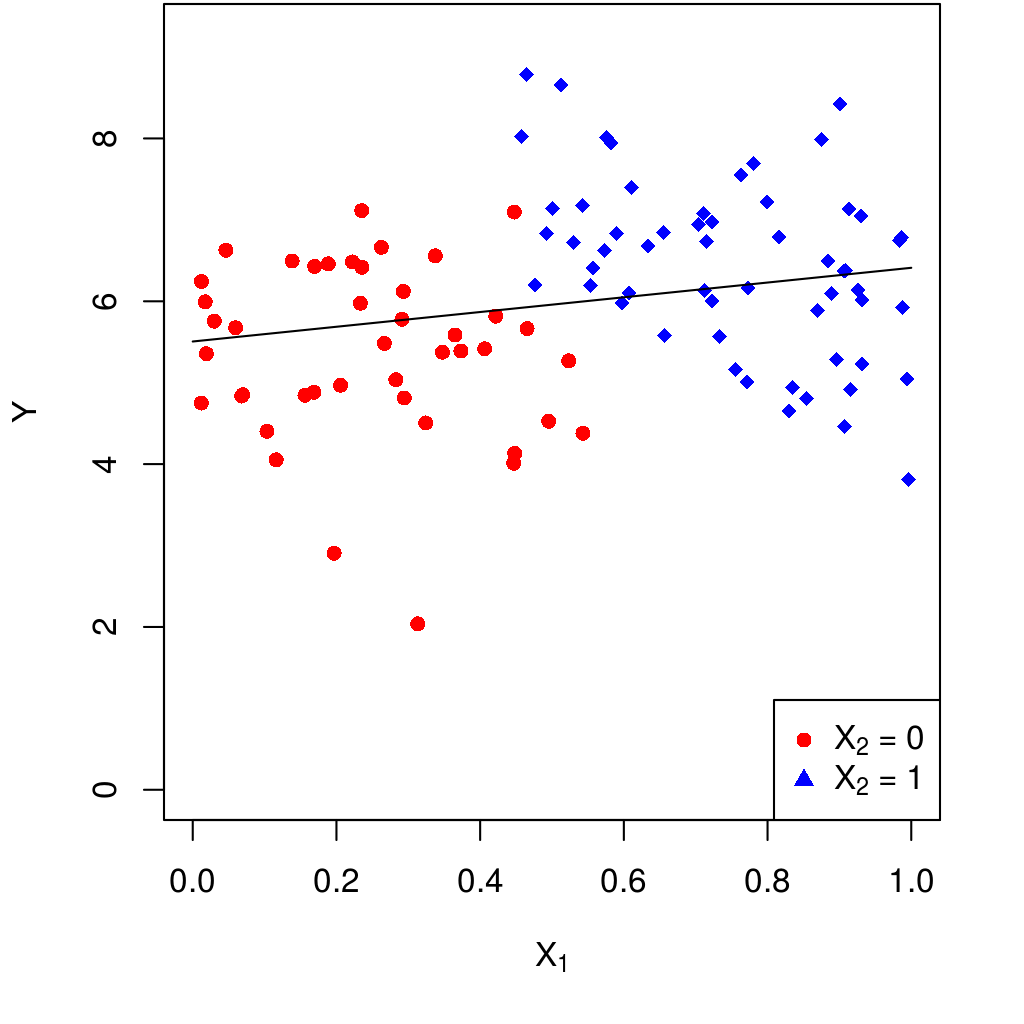
\includegraphics[width = 0.75\textwidth]{./plots/confounding_colored_with_simple_line.png}
\end{frame}

\begin{frame}
\frametitle{Multiple regression: motivation}
How about now?

\vspace{-0.3cm}
\centering
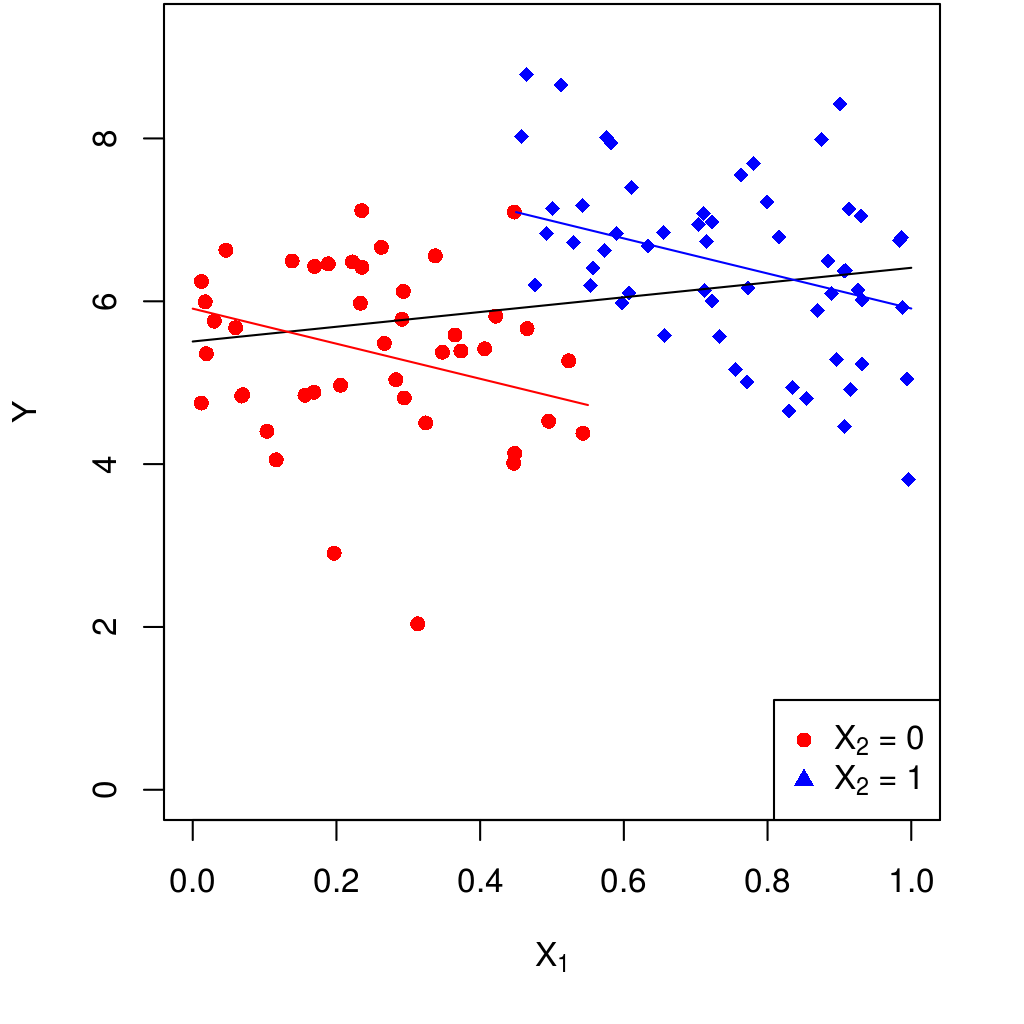
\includegraphics[width = 0.75\textwidth]{./plots/confounding_colored_with_lines.png}
\end{frame}

\begin{frame}
\frametitle{Multiple regression: motivation}
The true relationship between $Y$ and $X_1$ on the previous slides is 
\begin{align*}
E(Y \mid X_1) =& \ 6 - 2 X_1 \text{ in those with $X_2 = 0$, and } \\
E(Y \mid X_1) =& \ 8 - 2 X_1 \text{ in those with $X_2 = 1$}.
\end{align*}

What happened when we \textcolor{red}{did not account for} $X_2$ in the analysis? \pause {\small Hint: we estimated the \textbf{pooled} coefficient for $X_1$ to be 0.91}

\end{frame}

% Effect modification
\begin{frame}
\frametitle{Multiple regression: motivation}
What do you think the relationship is between $X_1$ and $Y$?

\centering
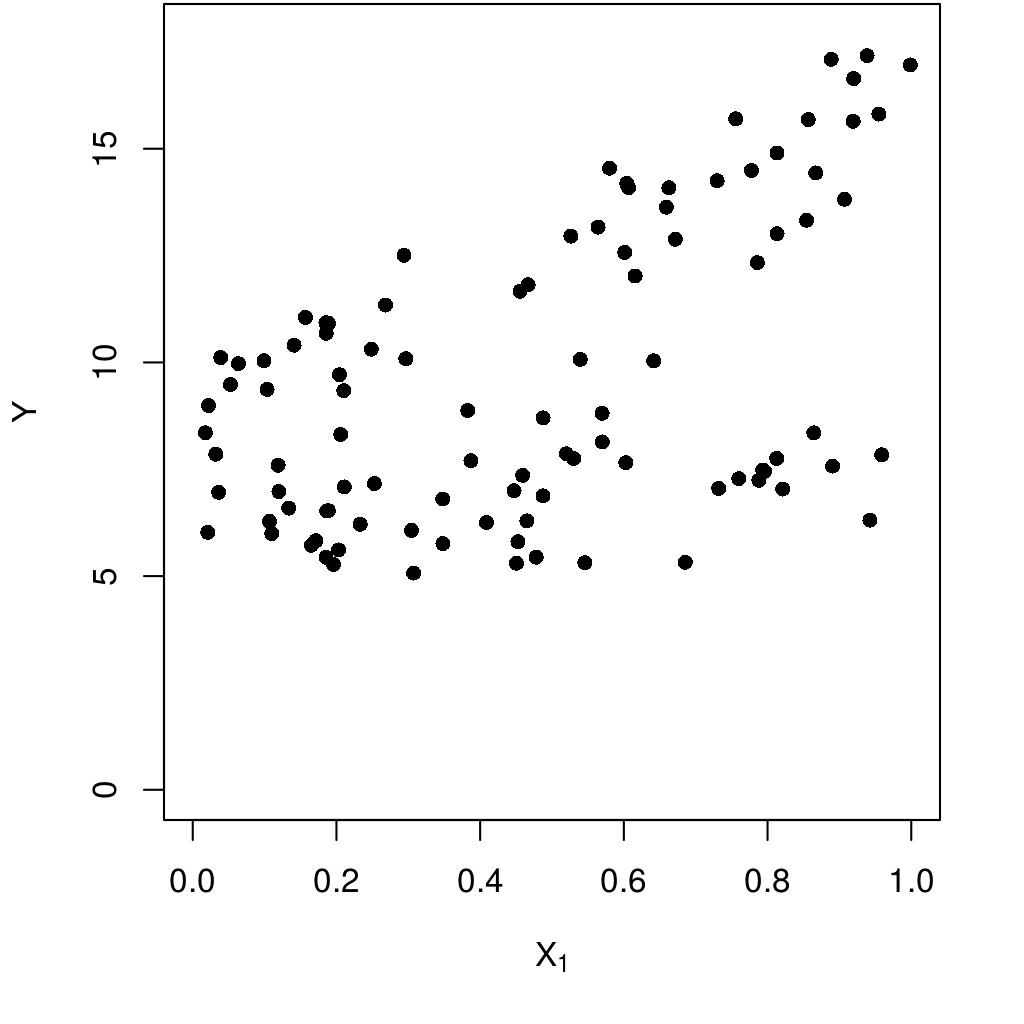
\includegraphics[width = 0.75\textwidth]{plots/effect_modification_simple.png}
\end{frame}

\begin{frame}
\frametitle{Multiple regression: motivation}
What do you think the relationship is between $X_1$ and $Y$?

\centering
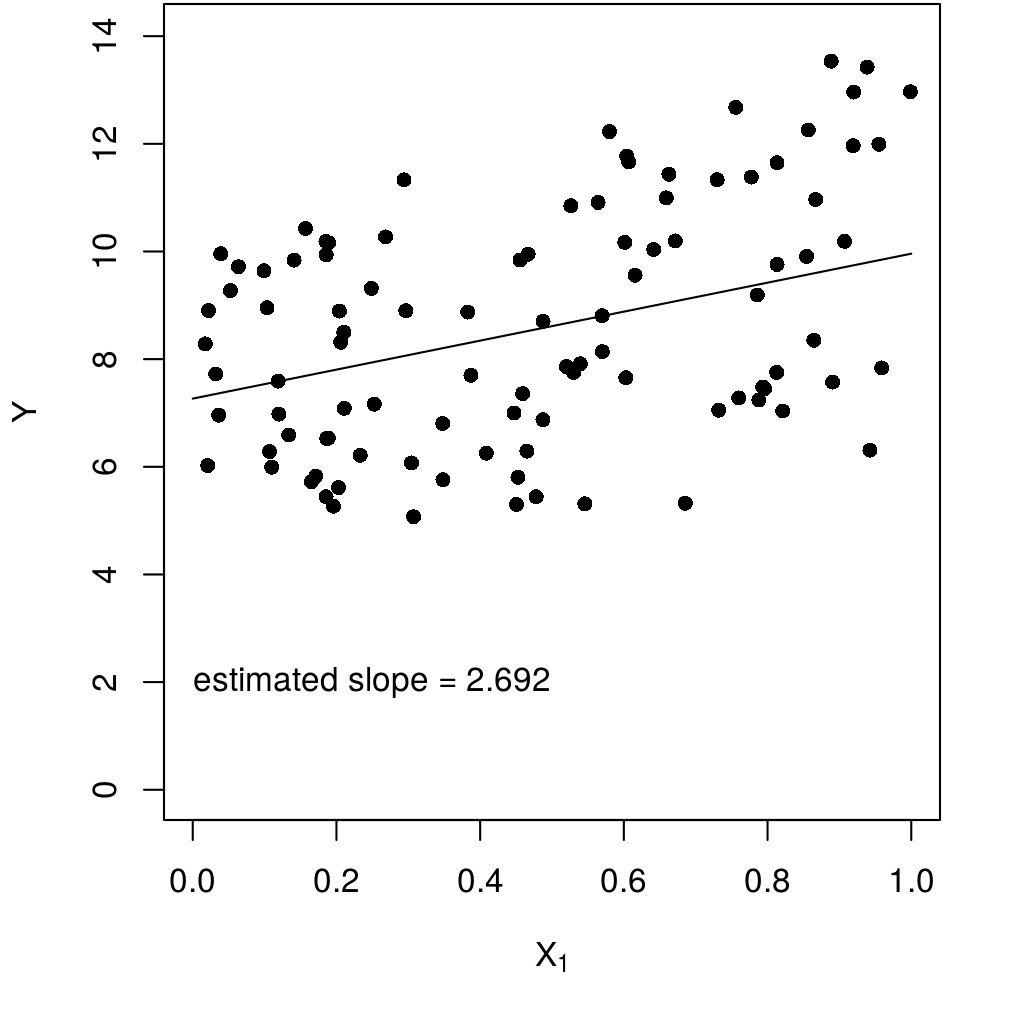
\includegraphics[width = 0.75\textwidth]{plots/effect_modification_simple_with_line.png}
\end{frame}

\begin{frame}
\frametitle{Multiple regression: motivation}
How about now?

\centering
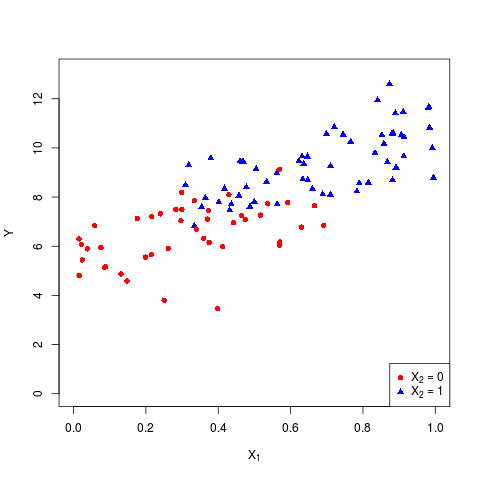
\includegraphics[width=0.75\textwidth]{plots/effect_modification_colored.png}

\end{frame}

\begin{frame}
\frametitle{Multiple regression: motivation}
How about now?

\centering
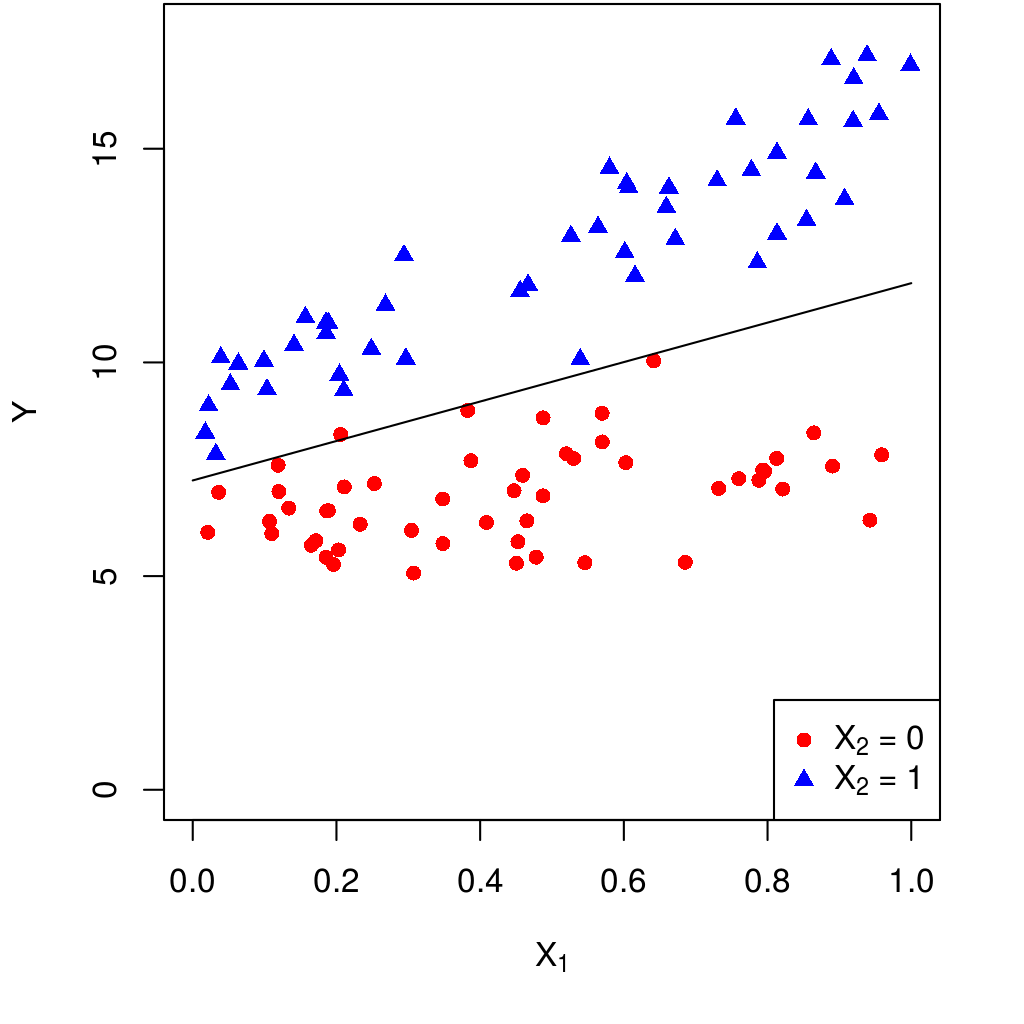
\includegraphics[width=0.75\textwidth]{plots/effect_modification_colored_with_simple_line.png}

\end{frame}

\begin{frame}
\frametitle{Multiple regression: motivation}
How about now?

\centering
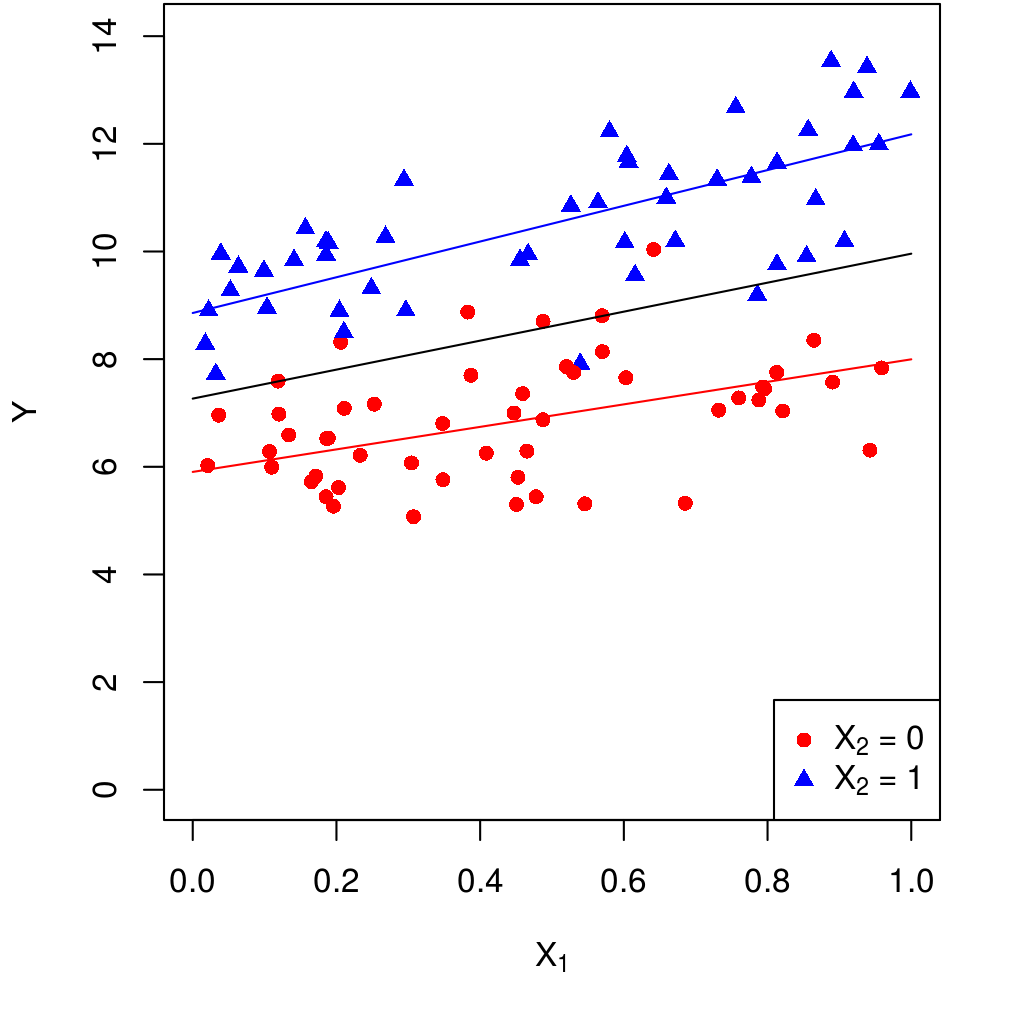
\includegraphics[width=0.75\textwidth]{plots/effect_modification_colored_with_lines.png}

\end{frame}

\begin{frame}
\frametitle{Multiple regression: motivation}
The true relationship between $Y$ and $X_1$ on the previous slides is 
\begin{align*}
E(Y \mid X_1) =& \ 6 + 2 X_1 \text{ in those with $X_2 = 0$, and } \\
E(Y \mid X_1) =& \ 9 + 7 X_1 \text{ in those with $X_2 = 1$}.
\end{align*}

What happened when we \textcolor{blue}{did not account for} $X_2$ in the analysis? \pause {\small Hint: we estimated the \textbf{pooled} coefficient for $X_1$ to be 2.62}
\end{frame}

% precision variables
\begin{frame}
\frametitle{Multiple regression: motivation}
What do you think the relationship is between $X_1$ and $Y$?

\centering
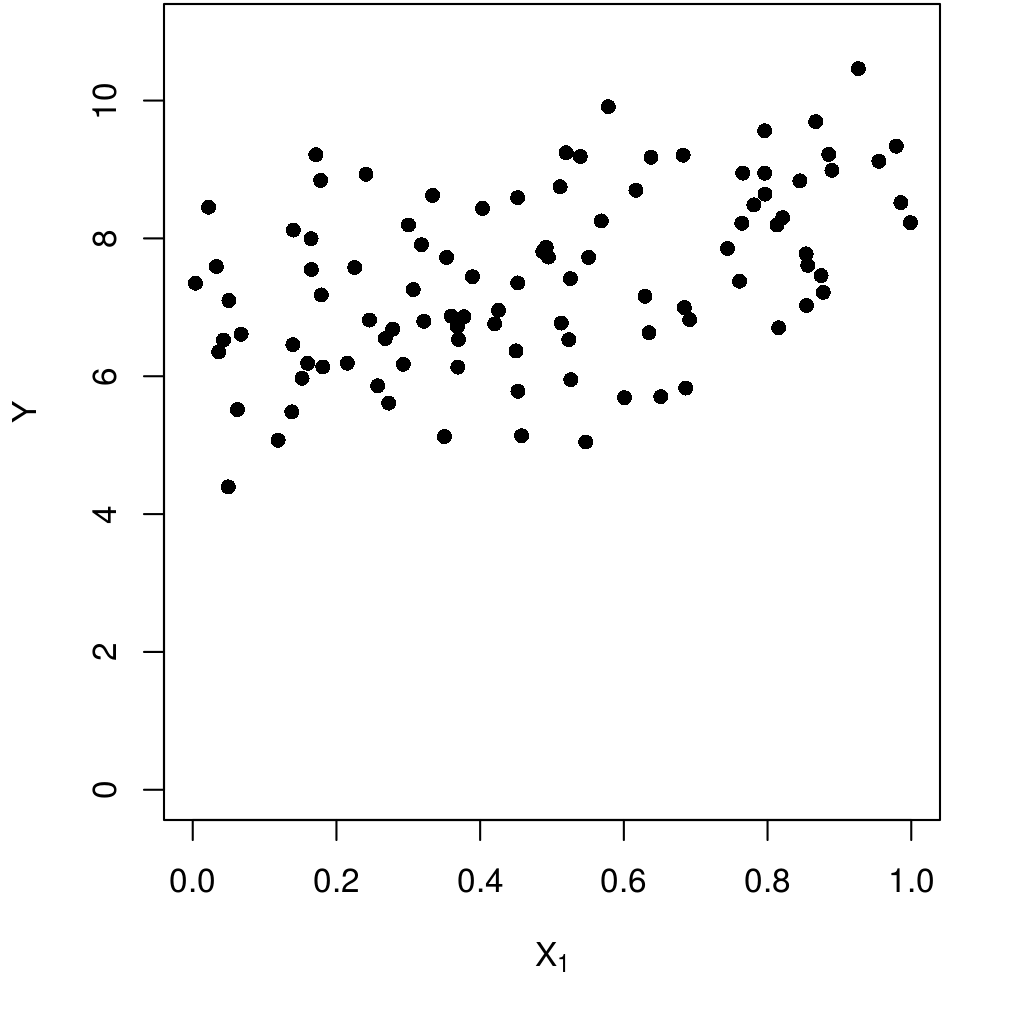
\includegraphics[width=0.75\textwidth]{plots/precision_simple.png}
\end{frame}

\begin{frame}
\frametitle{Multiple regression: motivation}
What do you think the relationship is between $X_1$ and $Y$?

\centering
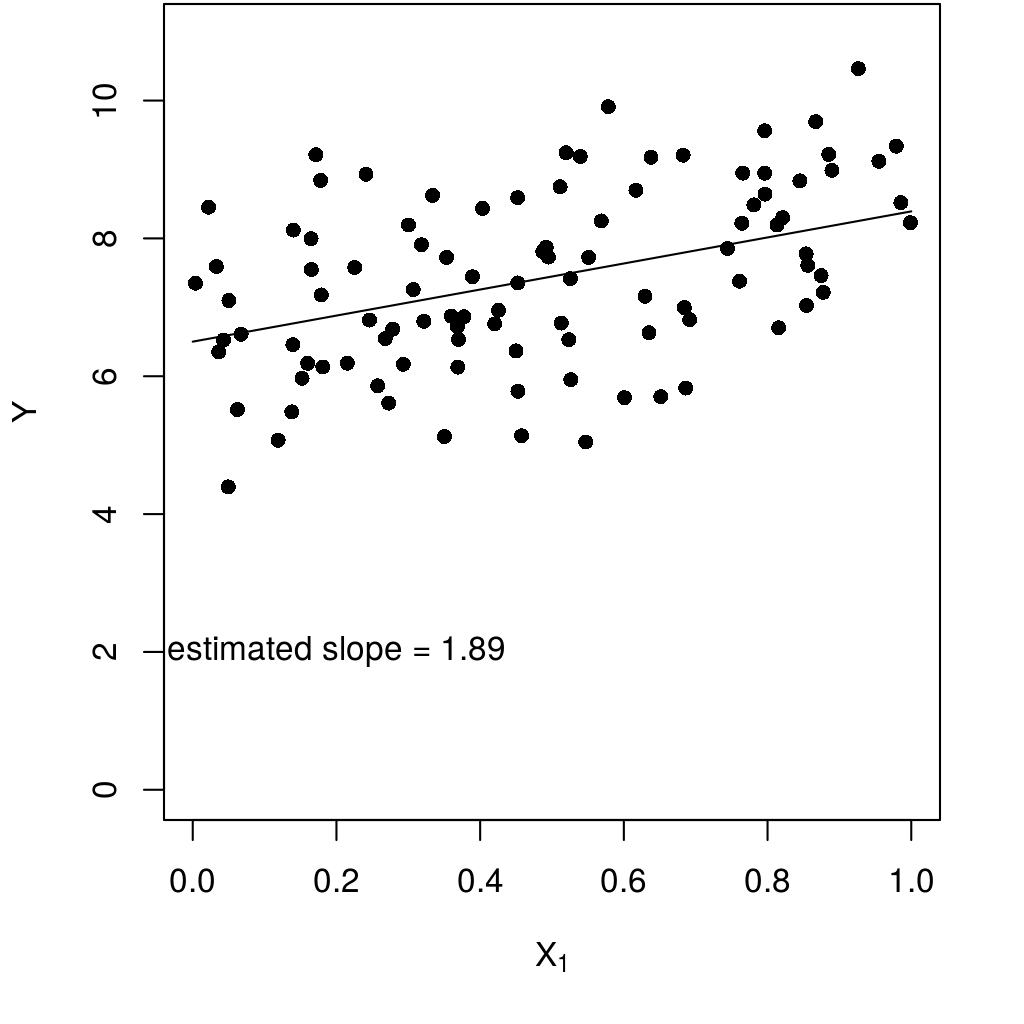
\includegraphics[width=0.75\textwidth]{plots/precision_simple_with_line.png}
\end{frame}

\begin{frame}
\frametitle{Multiple regression: motivation}
How about now?

\centering
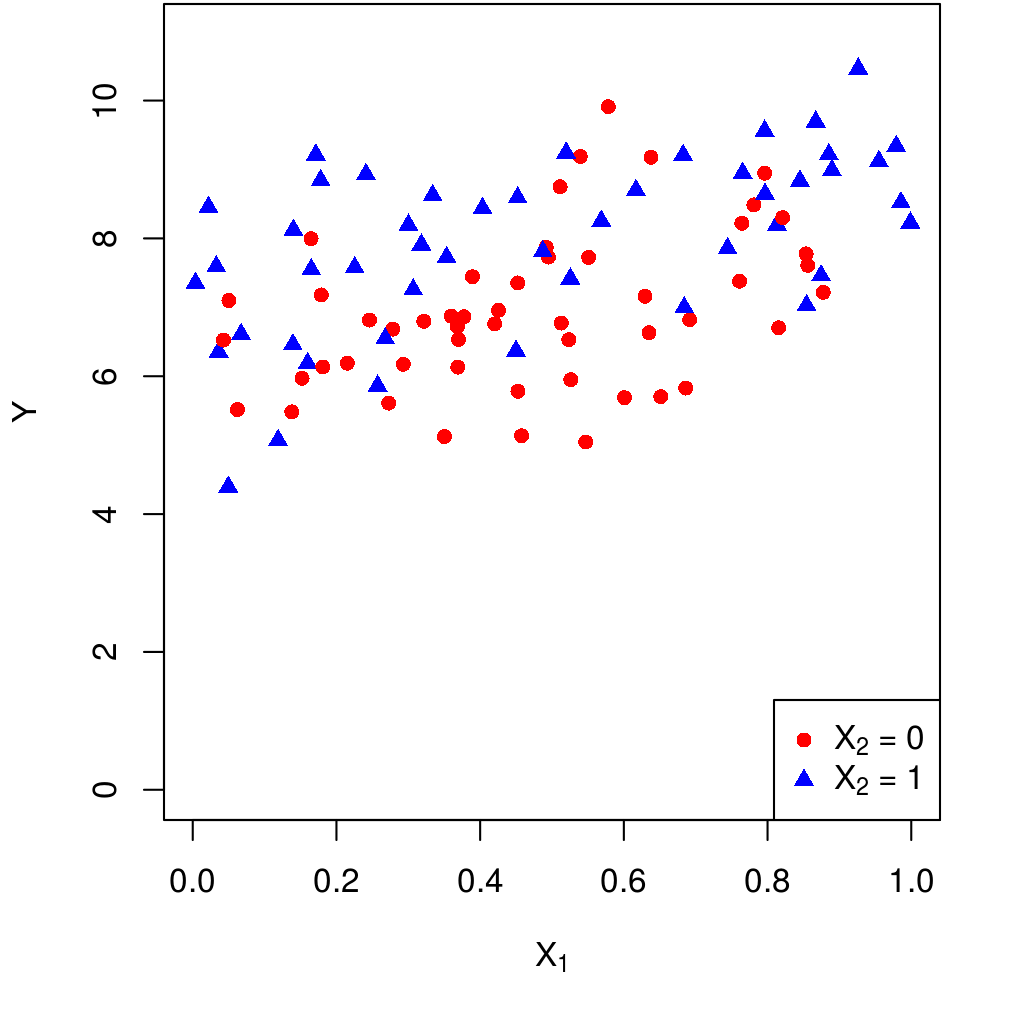
\includegraphics[width=0.75\textwidth]{plots/precision_colored.png}
\end{frame}

\begin{frame}
\frametitle{Multiple regression: motivation}
How about now?

\centering
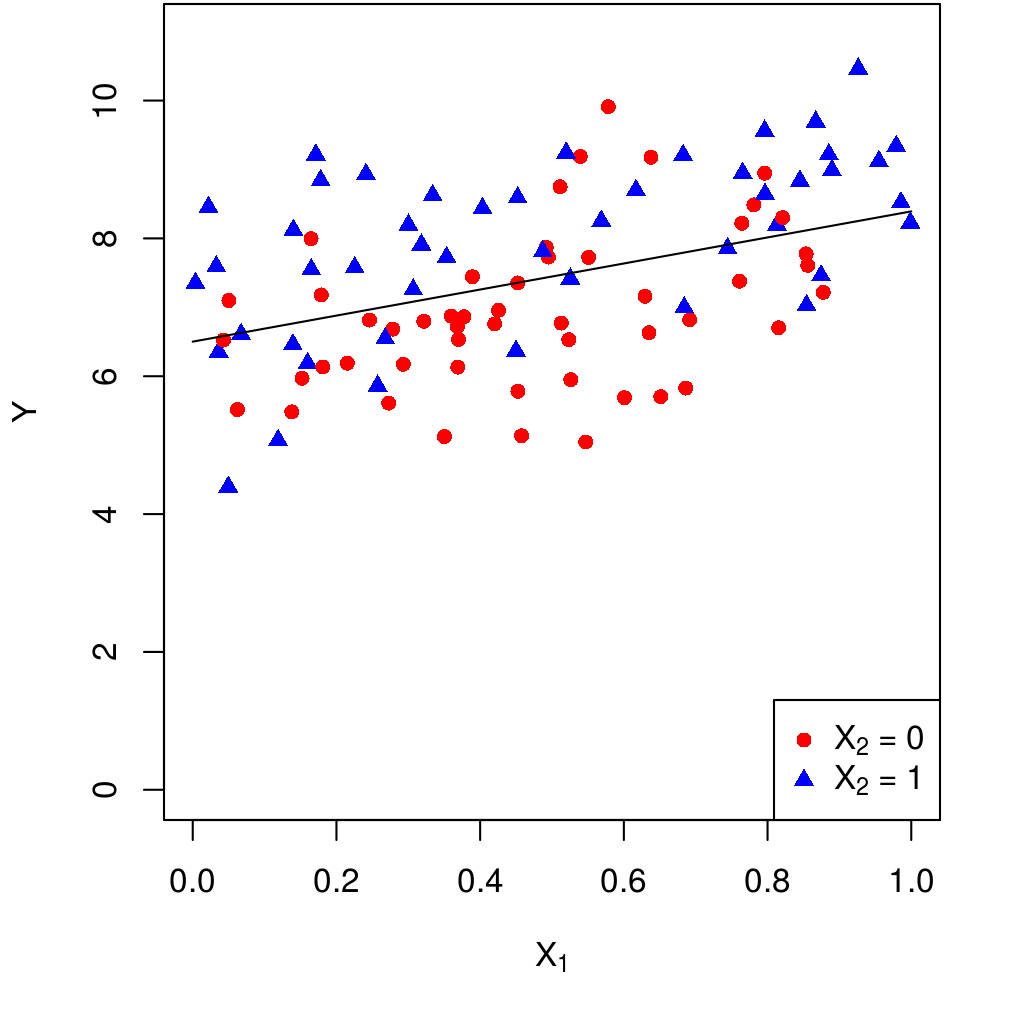
\includegraphics[width=0.75\textwidth]{plots/precision_colored_with_line.png}
\end{frame}

\begin{frame}
\frametitle{Multiple regression: motivation}
How about now?

\centering
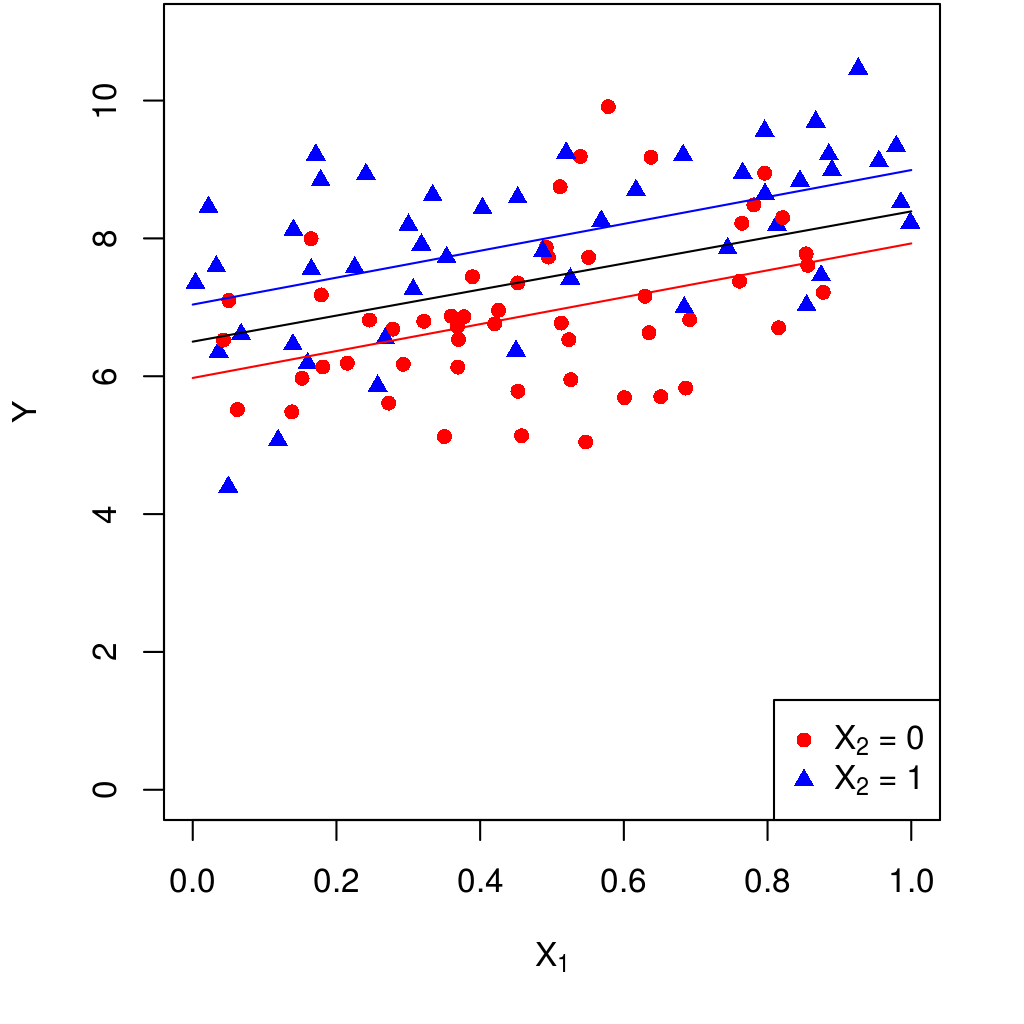
\includegraphics[width=0.75\textwidth]{plots/precision_colored_with_multiple_lines.png}
\end{frame}

\begin{frame}
\frametitle{Multiple regression: motivation}
The true relationship between $Y$ and $X_1$ on the previous slides is 
\begin{align*}
E(Y \mid X_1) =& \ 6 + 2 X_1 \text{ in those with $X_2 = 0$, and } \\
E(Y \mid X_1) =& \ 7 + 2 X_1 \text{ in those with $X_2 = 1$}.
\end{align*}

What happened when we \textcolor{green}{did not account for} $X_2$ in the analysis? \pause {\small Hint: we estimated the \textbf{pooled} coefficient for $X_1$ to be 1.89}
\end{frame}

\begin{frame}
\frametitle{Multiple regression: motivation}
Why spend so much time on linear regression?

\textcolor{red}{Confounders} (slides 1.66--1.71), \textcolor{blue}{effect modifiers} (slides 1.72--1.77), and \textcolor{green}{precision variables} (slides 1.77--1.83) all show up in other types of regression as well.

Additionally, the types of considerations we will have to make when choosing variables for our analysis, and the interpretation of regression coefficients, will be similar to those for linear regression in other regression types.

Linear regression is the most straightforward, so we'll spend a lot of time here!
\end{frame}

\subsection{Adjusting for covariates}
\begin{frame}
\frametitle{Adjusting for covariates}

Our statistical (and scientific) questions involve an \textbf{outcome} and a \textbf{predictor of interest}.

Scientific questions typically address one of three relationships between the predictor of interest and the outcome: \vspace{-0.2cm}
\begin{itemize}
\item is there a causal association?
\item is there an association?
\item does the association (if it exists) differ in groups defined by an additional covariate? (\textcolor{blue}{effect modification})
\end{itemize}

Study designs can be broadly categorized as observational or randomized and controlled.

\textcolor{red}{Depending on the scientific question and the study design}, we may need to \textcolor{red}{consider additional variables} (from now on, called \textbf{covariates}).

\end{frame}

\begin{frame}
\frametitle{Adjusting for covariates: terminology}

If these additional variables can potentially impact our ability to estimate a causal association \textcolor{red}{(confounders)}, or define our scientific question \textcolor{blue}{(effect modifiers)}, then we need to include these variables in our analysis---this is called \textbf{adjusting}.

Simple linear regression: 
\begin{itemize}
\item compare the average outcome across groups which have different values for the predictor of interest
\end{itemize}

Multiple linear regression:
\begin{itemize}
\item compare the average outcome across groups which have different values for the predictor of interest, \pause and 
\item have the same value for all other covariates in the model
\end{itemize}
\end{frame}

\begin{frame}
\frametitle{Types of covariates: confounders}

\textcolor{red}{Confounder}: causally associated with the outcome \textbf{in the population}; associated with the predictor of interest \textbf{in our sample}; not a result of the predictor of interest.

\centering
\vspace{-0.1cm}
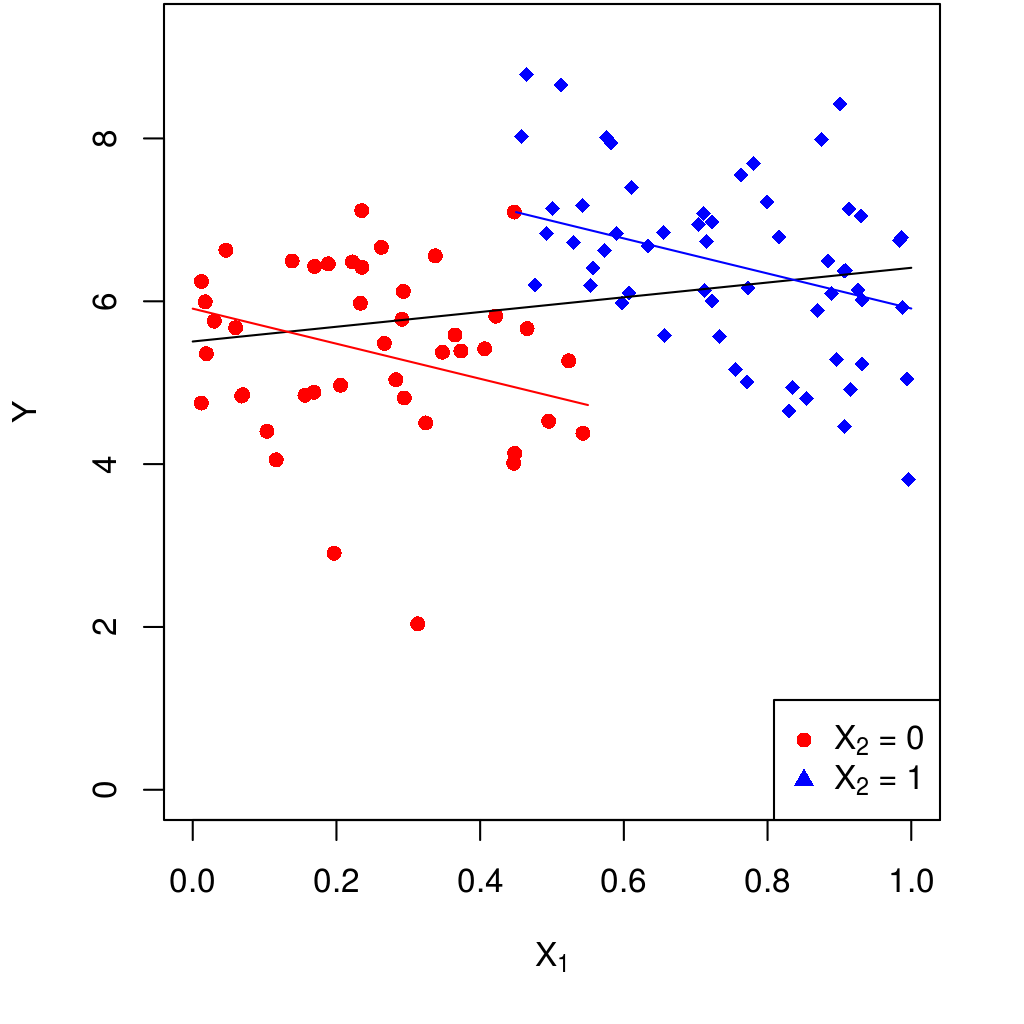
\includegraphics[width=0.65\textwidth]{plots/confounding_colored_with_lines.png}

\end{frame}

\begin{frame}
\frametitle{Types of covariates: confounders}
\textcolor{red}{Confounder}: causally associated with the outcome \textbf{in the population}; associated with the predictor of interest \textbf{in our sample}; not a result of the predictor of interest.

Classical confounder:

\begin{center}
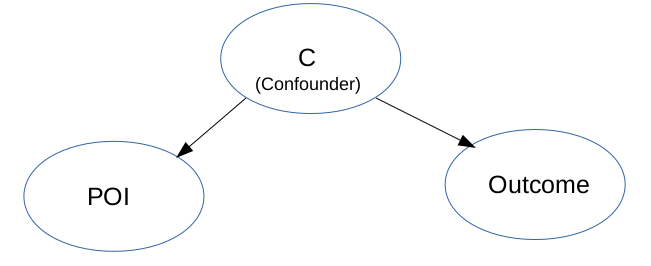
\includegraphics[width=0.7\textwidth]{plots/classical_confounder.png}
\end{center}

\end{frame}

\begin{frame}
\frametitle{Types of covariates: confounders}
\textcolor{red}{Confounder}: causally associated with the outcome \textbf{in the population}; associated with the predictor of interest \textbf{in our sample}; not a result of the predictor of interest.

Causal pathway (not a confounder!):

\begin{center}
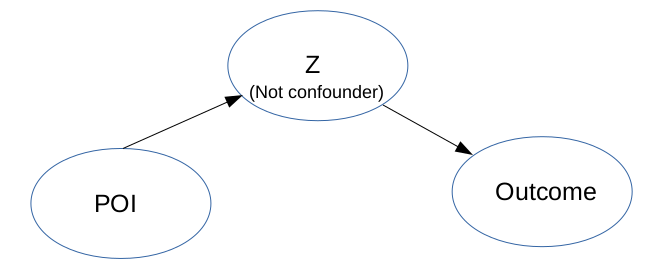
\includegraphics[width=0.7\textwidth]{plots/causal_pathway.png}
\end{center}

\end{frame}

\begin{frame}
\frametitle{Types of covariates: confounders}
\textcolor{red}{Confounder}: causally associated with the outcome \textbf{in the population}; associated with the predictor of interest \textbf{in our sample}; not a result of the predictor of interest.

Surrogate for response (not a confounder!):

\begin{center}
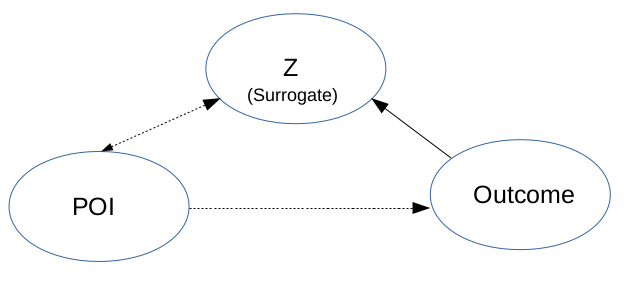
\includegraphics[width=0.7\textwidth]{plots/surrogate.png}
\end{center}

\end{frame}

\begin{frame}
\frametitle{Types of covariates: effect modifiers}

\textcolor{blue}{Effect modifier}: the association between the outcome and the predictor of interest \textbf{depends on the value} of the effect modifier.

\centering
\vspace{-0.2cm}
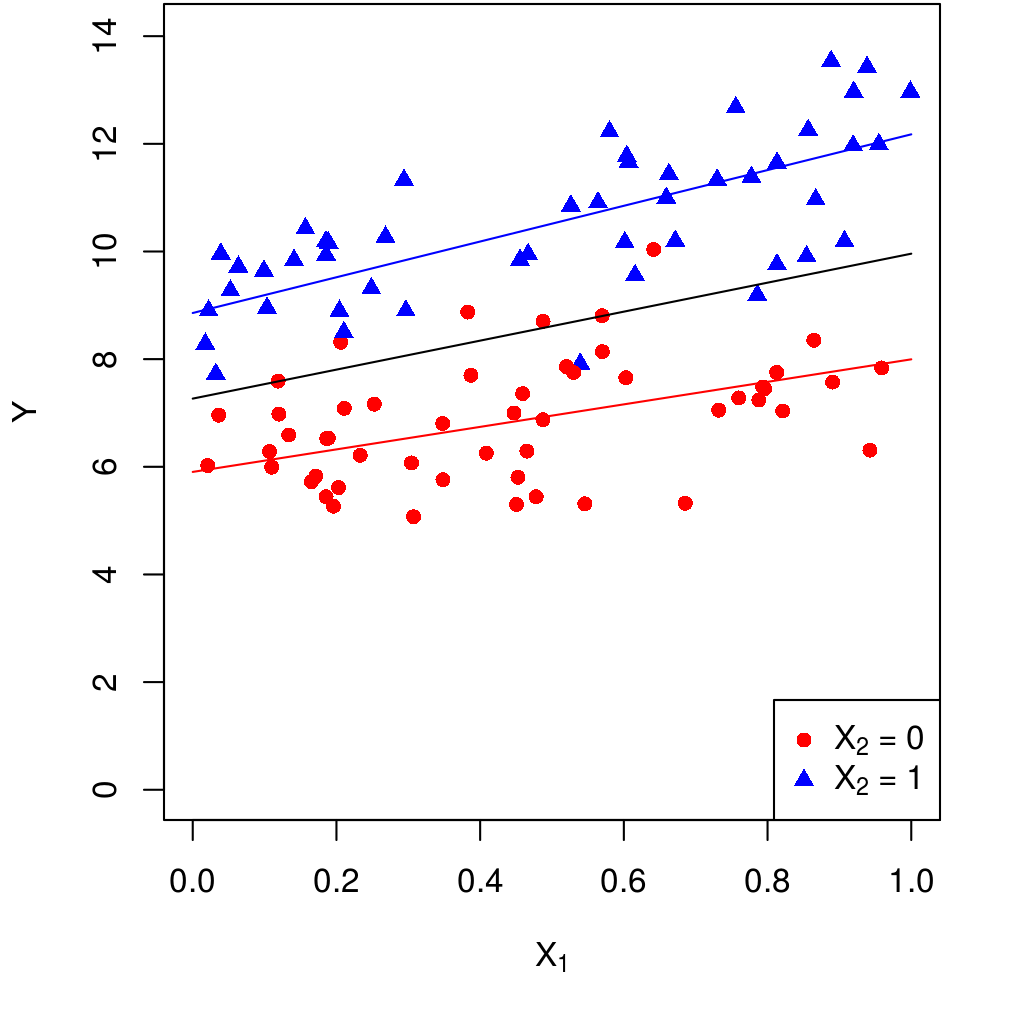
\includegraphics[width=0.65\textwidth]{plots/effect_modification_colored_with_lines.png}
\end{frame}

\begin{frame}
\frametitle{Types of covariates: precision variables}

\textcolor{green}{Precision variable}: associated with the outcome in the population; \textbf{not associated with} the predictor of interest \textbf{in the sample}.

\centering
\vspace{-0.2cm}
 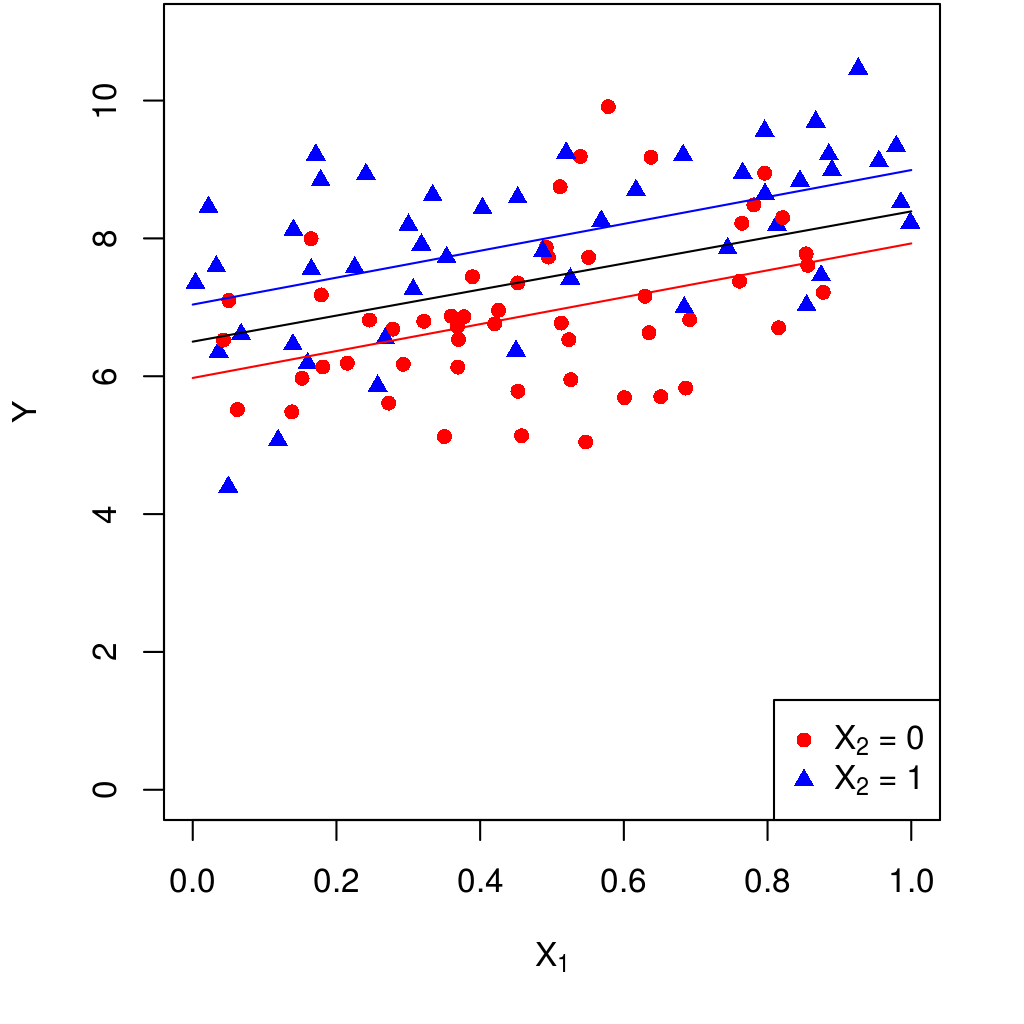
\includegraphics[width=0.65\textwidth]{plots/precision_colored_with_multiple_lines.png}
\end{frame}


\begin{frame}
\frametitle{Adjusting for covariates: causal diagrams}
Often, when thinking about the need to adjust for additional covariates, it is helpful to draw a \textbf{causal diagram} relating the outcome, predictor of interest, and additional covariates.

Here, the \textbf{nodes} (or vertices) denote variables, and the \textbf{edges} between these nodes denote associations. Arrows denote \textcolor{blue}{causal} associations.

For example, consider the relationship between FEV (the outcome) and smoking status (the predictor of interest). Additional variables we might consider are age, sex, and height. 

Our scientific question is: is there an association between FEV and smoking status? {\small (assume we are after causality, but cannot get it due to study design)}
\end{frame}

\begin{frame}
\frametitle{Adjusting for covariates: causal diagrams \\ {\small page intentionally blank, for FEV example}}


\end{frame}

\begin{frame}
\frametitle{Adjusting for covariates: causal association}

When our scientific question involves a causal association, whether or not we need to adjust for covariates \textbf{depends on the study design}. \vspace{-0.4cm}
\begin{itemize}
\item Randomized controlled trial: \textcolor{blue}{no need to adjust}, in general, for large sample size
\item Observational study: \textcolor{red}{always need to adjust} for potential confounders
\end{itemize}

In an observational study: \vspace{-0.4cm}
\begin{itemize}
\item groups defined by different values of your predictor of interest may be different in other ways
\item these variables that differ between groups may affect your outcome
\item any association you see could be due to the predictor of interest, but could also be due to one of the other variables that differs between groups
\end{itemize}
\end{frame}

\begin{frame}
\frametitle{Adjusting for covariates: causal association}

In this course, most of our scientific questions will involve a causal association, e.g., \textcolor{red}{is systolic blood pressure associated with age?}

However, if we do not have data from an RCT, we may draw the wrong conclusions if we do not account for potential confounders. 

Thus we change our question to, e.g., \textcolor{blue}{is systolic blood pressure associated with age, adjusting for gender and BMI?}

Thus, when we estimate the association between the predictor of interest and the outcome, we want to do so at \textbf{fixed values} of the confounder.
\end{frame}

\begin{frame}
\frametitle{Adjusting for covariates: association}
When our scientific question involves an association (not causal!), we \textbf{rarely need to adjust} for covariates. Here, our goal is to see if there is any association; we aren't concerned with whether or not this association is due to other variables. 

However, we may choose to adjust to: \vspace{-0.3cm}
\begin{itemize}
\item reduce the variability in our estimates \textcolor{green}{(precision variables)}
\item get a better prediction of the mean outcome (more on this later)
\end{itemize}

Example: designing an intervention \vspace{-0.3cm}
\begin{itemize}
\item if we have a \textcolor{blue}{cheap, easy to measure} predictor, 
\item and our outcome \textbf{is associated with} this predictor,
\item then we know who to target \textbf{regardless of the underlying causal mechanism}
\end{itemize}
\end{frame}

\begin{frame}
\frametitle{Adjusting for covariates: effect modification}

When our scientific question addresses whether or not a (causal) association differs in strata defined by another covariate, we \textbf{must adjust} for this covariate (otherwise, we would not be answering the question).

This phenomenon is also called a \textcolor{blue}{subgroup effect}, or statistically, an \textcolor{blue}{interaction}.

\end{frame}

\begin{frame}
\frametitle{Adjusting for covariates: summary}
Whether or not we need to adjust for covariates depends on: \vspace{-0.2cm}
\begin{itemize}
\item the scientific question (causal? effect modification?)
\item the study design (RCT vs observational)
\end{itemize}

The types of covariates we might adjust for (based on science) are: \vspace{-0.2cm}
\begin{itemize}
\item \textcolor{red}{confounders}
\item \textcolor{blue}{effect modifiers}
\item \textcolor{green}{precision variables}
\end{itemize}

Next, we'll see how to interpret coefficients in adjusted analyses, and how to use \texttt{R} to fit multiple linear regression models. We'll also see many examples of all three types of covariates.
\end{frame}


\subsection{Stratified analyses}
\begin{frame}
\frametitle{Stratified analyses: ``multiple'' regression}
Say we are interested in \textcolor{blue}{estimating the association} between an outcome, $Y$, and a predictor of interest $X$; however, knowledge of the scientific problem tells us that a third variable $Z$ may be related to $Y$ and/or $X$.

If $Z$ is \textbf{binary}, how might we account for it? \pause
One way to account for a second predictor variable is to \textbf{stratify} our analysis:
\begin{itemize}
\item Fit a linear regression of $Y$ on $X$ for those with $Z = 0$
\item Fit a linear regression of $Y$ on $X$ for those with $Z = 1$
\end{itemize}

\end{frame}

\begin{frame}
\frametitle{Stratified analyses: interpretation}
\vspace{-2cm}This implies the following two regression models:
\begin{align*}
E(Y \mid X, Z = 0) &= \beta_0 + \beta_1 X, \text{ and } \\
E(Y \mid X, Z = 1) &= \gamma_0 + \gamma_1 X.
\end{align*}

What is the interpretation of $\beta_0$? $\gamma_0$?
\end{frame}

\begin{frame}
\frametitle{Stratified analyses: interpretation}
\vspace{-2cm}This implies the following two regression models:
\begin{align*}
E(Y \mid X, Z = 0) &= \beta_0 + \beta_1 X, \text{ and } \\
E(Y \mid X, Z = 1) &= \gamma_0 + \gamma_1 X.
\end{align*}

What is the interpretation of $\beta_1$? $\gamma_1$?
\end{frame}

\begin{frame}
\frametitle{Stratified analyses: FEV}

Is smoking associated with FEV, \textcolor{red}{adjusted for height}?

Linear regression model, stratifying on height $< 60$ inches versus height $\geq 60$ inches:
\begin{align*}
E(\text{FEV} \mid \text{Smoker}, \text{Height} < 60) &= \beta_0 + \beta_1 \text{Smoker} \\
E(\text{FEV} \mid \text{Smoker}, \text{Height} \geq 60) &= \gamma_0 + \gamma_1 \text{Smoker} 
\end{align*}

To estimate the regression coefficients, we will need to: create two new subsets of the data, corresponding to $< 60$ and $\geq 60$ inches; and fit a linear regression of FEV on smoking status within each stratum.
\end{frame}

\begin{frame}
\frametitle{Stratified analyses: FEV}

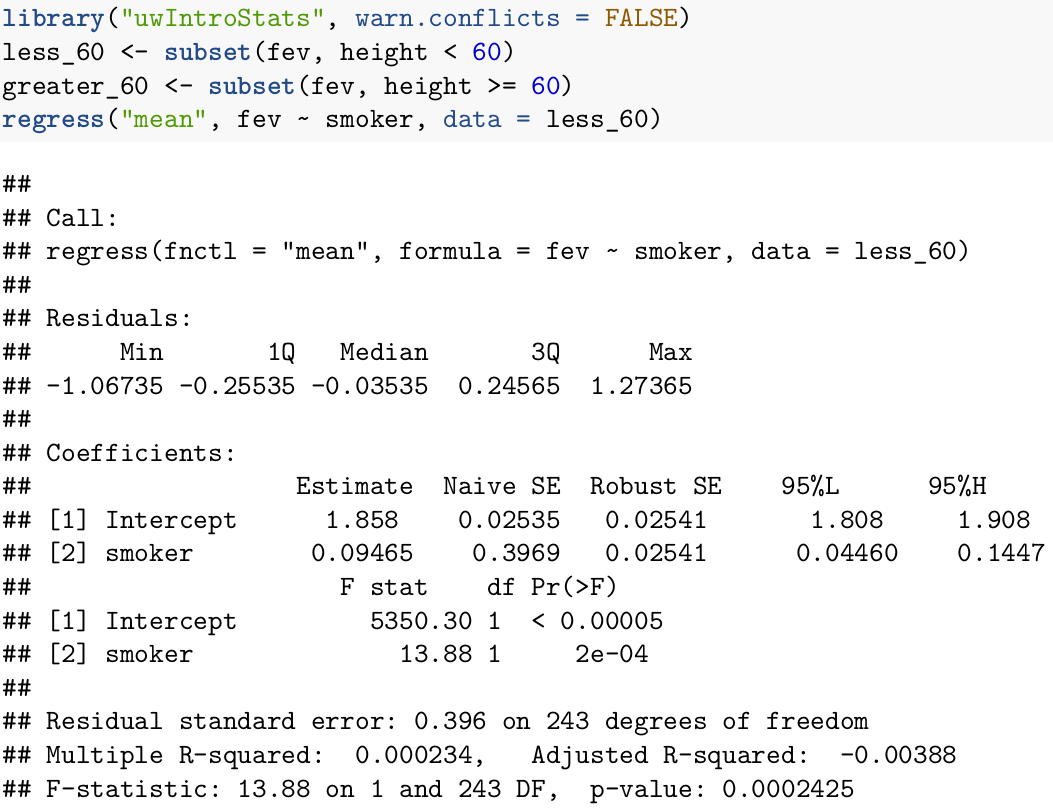
\includegraphics[width=1\textwidth]{plots/fev_vs_smoke_stratified_less_60.png}

\end{frame}

\begin{frame}
\frametitle{Stratified analyses: FEV}

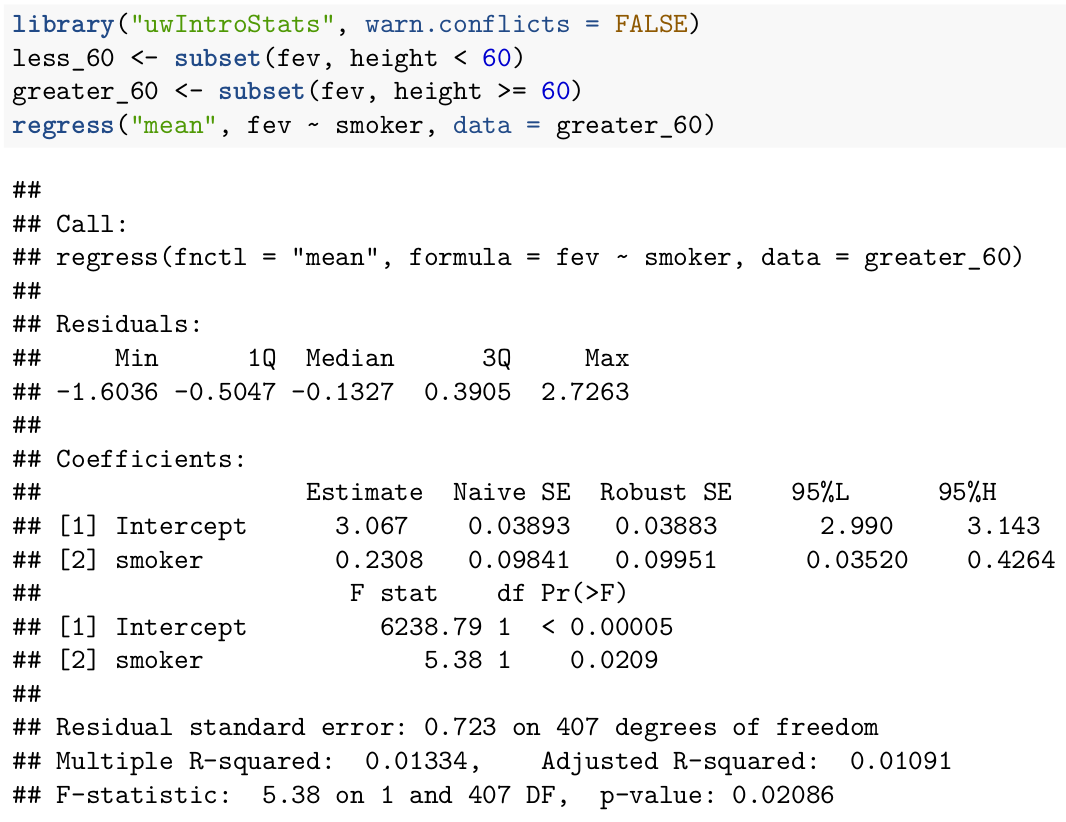
\includegraphics[width=1\textwidth]{plots/fev_vs_smoke_stratified_greater_60.png}

\end{frame}

\begin{frame}
\frametitle{Stratified analyses: FEV}
\vspace{-1cm}\hspace*{-0.75cm}\begin{tabular}{lll}
& \multicolumn{2}{c}{Estimated coefficient [95\% CI]} \\
Analysis & Smoke & Intercept \\
\hline
Unadjusted  & 0.71 [0.52, 0.90] & 2.57 \\
Stratified: height $< 60$ & 0.095 [0.045, 0.145] & 1.86\\
Stratified: height $\geq 60$ & 0.231 [0.035, 0.426] & 3.07
\end{tabular}

\vspace{1cm}
When comparing the unadjusted analysis to the stratified analysis, what do you notice? What does this suggest, in light of your causal diagram (1.94)?
\end{frame}

\begin{frame}
\frametitle{Stratified analyses: summary}
Stratified analyses are similar to using a t-test:
\begin{itemize}
\item a valid way of analyzing your data
\item straightforward if the stratification variable is already binary
\item a bit arbitrary if the stratification variable is continuous
\end{itemize}

As you saw in Homework 3, using the t-test is equivalent to simple linear regression with a binary predictor---similarly, with only two variables, a \textcolor{blue}{stratified analysis is approximately equivalent to a multiple linear regression analysis} if the stratification variable is binary. 
\end{frame}

\subsection{Multiple linear regression}
\begin{frame}
\frametitle{Multiple linear regression: two predictors}
In simple linear regression, we modeled the expected value of $Y$ given a single predictor $X$ as a linear function of the intercept and slope:
\begin{align*}
E(Y \mid X) &= \beta_0 + \beta_1 X,
\end{align*}
with independent observations.

How might you add in an additional variable, $Z$? \pause
\begin{align*}
E(Y \mid X, Z) &= \beta_0^* + \beta_1^* X + \beta_2^* Z,
\end{align*}
still with independent observations.

Estimates and confidence intervals are computed in the same way as in simple linear regression; \textbf{as before, your software can handle this}.
\end{frame}

\begin{frame}
\frametitle{Multiple linear regression: FEV, two predictors}
Multiple linear regression in action (with binary height): \vspace{-0.45cm}
\begin{center}
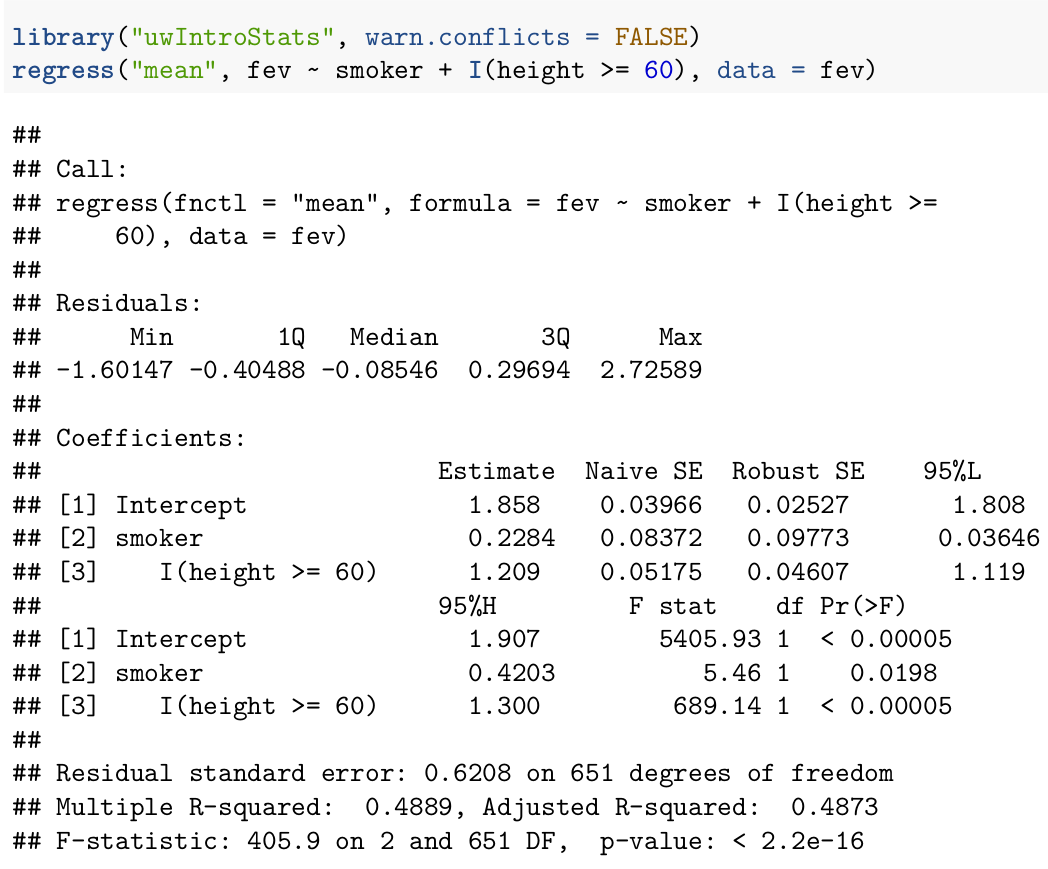
\includegraphics[width=0.85\textwidth]{plots/fev_vs_smoke_adjust_binary_height.png}
\end{center}
\end{frame}

\begin{frame}
\frametitle{Multiple linear regression: two predictors}
\begin{align*}
E(Y \mid X, Z) &= \beta_0^* + \beta_1^* X + \beta_2^* Z
\end{align*}

To interpret coefficients, we now have to \textbf{fix the value} of one covariate, and let the other change.

For example, in this model $\beta_1^*$ is interpreted as the difference in average $Y$ between two groups differing by one unit in $X$, but having the same value of $Z$. (Why?)

We now \textcolor{blue}{borrow information} across levels of $Z$: nearby values of $Z$ should provide some relevant information about the current value of $Z$ (e.g., 67 and 69 year olds should provide some relevant information for 68 year olds).

\end{frame}

\begin{frame}
\frametitle{Multiple linear regression: two predictors}
\centering
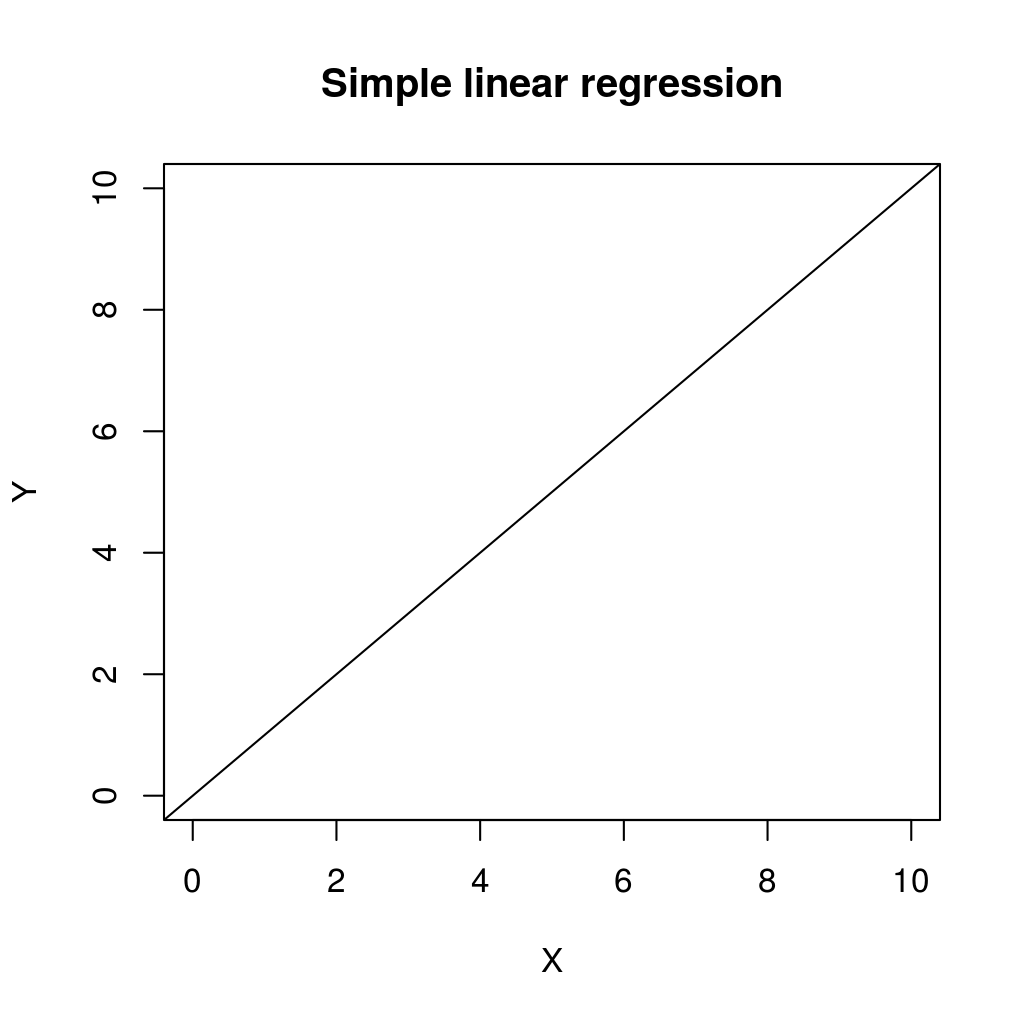
\includegraphics[width = 0.65\textwidth]{plots/simple_line.png}

$E(Y \mid X) = 0 + 1 X$
\end{frame}

\begin{frame}
\frametitle{Multiple linear regression: two predictors}
\centering
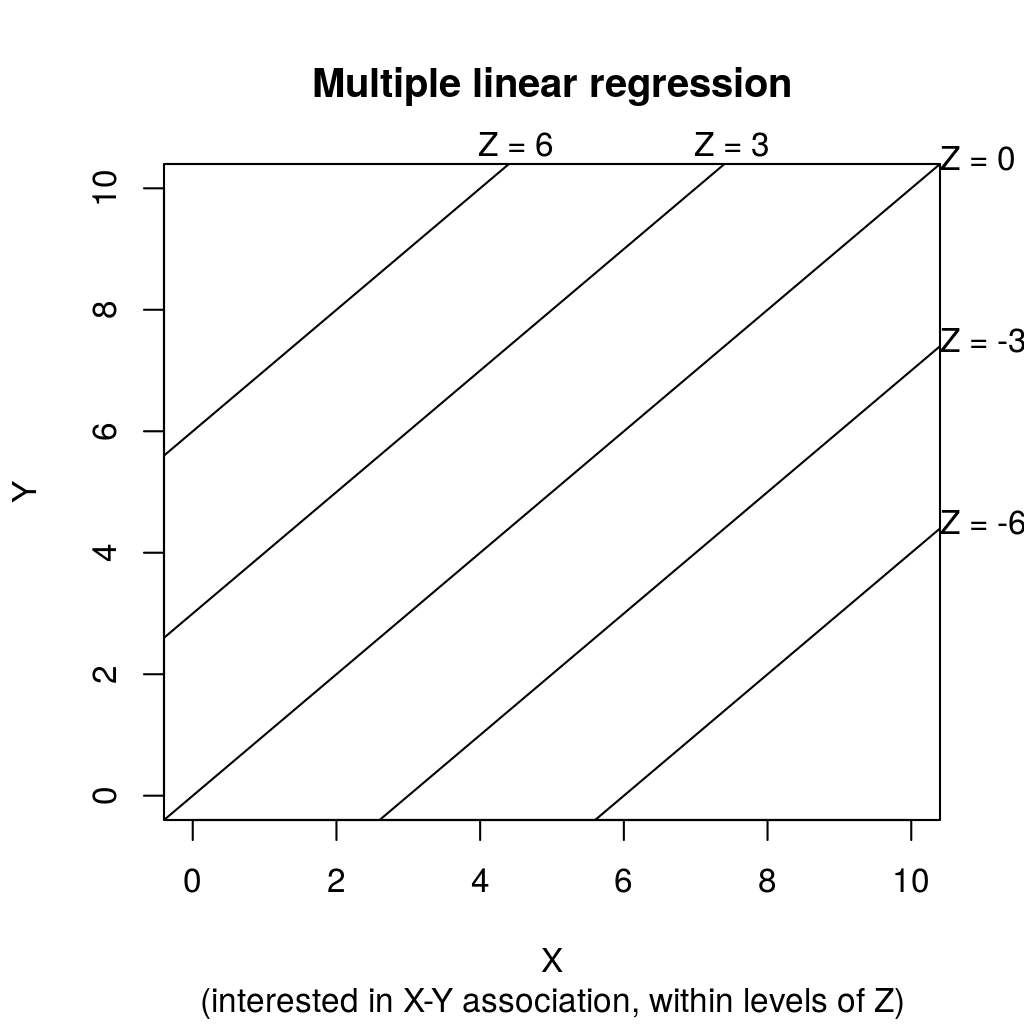
\includegraphics[width = 0.65\textwidth]{plots/multiple_line.png}

$E(Y \mid X, Z) = 0 + 1 X + 1 Z$
\end{frame}

\begin{frame}
\frametitle{Multiple linear regression: two predictors}

Mathematically, we can play the same game we did in simple linear regression: fixing $Z = z$, 
\begin{align*}
E\{Y \mid X = (x + 1), Z = z\} &= \beta_0^* + \beta_1^* (x + 1) + \beta_2^* z \\
E(Y \mid X = x, Z = z) &= \beta_0^* + \beta_1^* x + \beta_2^* z \\
E\{Y \mid X = (x + 1), Z = z\} & \\
- E(Y \mid X = x, Z = z) &= \beta_1^*
\end{align*}

In light of this, what is the interpretation of $\beta_0^*$? $\beta_2^*$? \vspace{2cm}
\end{frame}

\begin{frame}
\frametitle{Multiple linear regression: FEV, two predictors}
Multiple linear regression in action (with continuous height): \vspace{-0.45cm}
\begin{center}
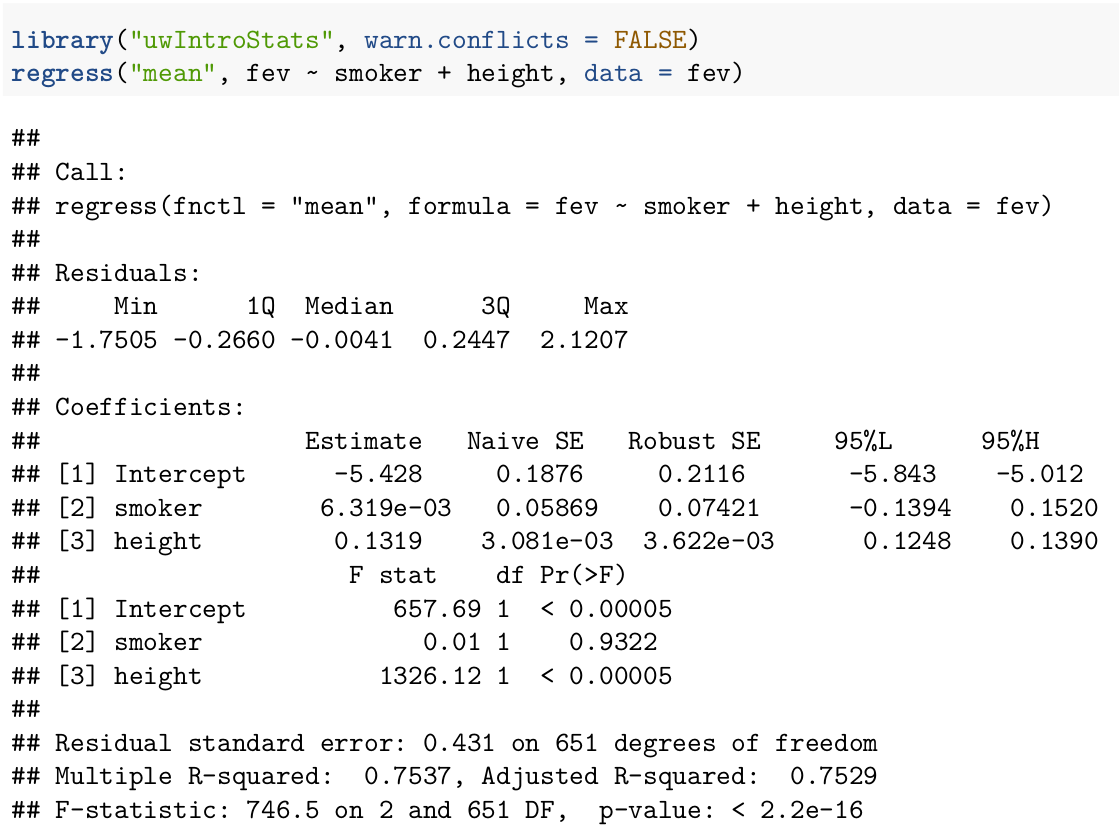
\includegraphics[width = 0.85\textwidth]{plots/fev_vs_smoke_adjust_height.png}
\end{center}
\end{frame}

\begin{frame}
\frametitle{Multiple regression vs stratifying: FEV}
\vspace{-1cm}\hspace*{-0.75cm}\begin{tabular}{llll}
& \multicolumn{3}{c}{Estimated coefficient [95\% CI]} \\
Analysis & Smoke & Height & Intercept \\
\hline
Unadjusted  & 0.71 [0.52, 0.90] & & 2.57\\
Height $< 60$ & 0.095 [0.045, 0.145]& & 1.86\\
Height $\geq 60$ & 0.231 [0.035, 0.426]& & 3.07 \\
Binary height & 0.228 [0.035, 0.420] & 1.21 [1.12, 1.30] & 1.86\\
Cont. height & 0.0062 [-0.139, 0.152]& 0.13 [0.12, 0.14] & -5.43
\end{tabular}

\begin{itemize}
\item Multiple with binary height \textcolor{blue}{similar to} stratified
\item Model height as continuous: no statistically significant effect (why?)
\end{itemize} 
\end{frame}

\begin{frame}
\frametitle{Multiple linear regression: many predictors}
Now we model the expected value of the response $Y$, given predictors $X_1, X_2, \dots, X_p$, as a \textcolor{cyan}{linear function of $p$ coefficients}:
\begin{align*}
E(Y \mid X_1, X_2, \dots, X_p) &= \beta_0 + \beta_1 X_1 + \beta_2 X_2 + \dots + \beta_p X_p, \text{ or } \\
&= \beta_0 + \sum_{j=1}^p \beta_j X_j,
\end{align*} 
where the observations are independent.

\textcolor{cyan}{Interpretation for $\beta_1$: the average difference in $Y$ values comparing two groups having the same value of $X_2, \dots, X_p$ but differing in $X_1$ by one unit.}

\end{frame}

\begin{frame}
\frametitle{Multiple linear regression: many predictors}
\begin{align*}
E(Y \mid X_1, X_2, \dots, X_p) &= \beta_0 + \beta_1 X_1 + \beta_2 X_2 + \dots + \beta_p X_p
\end{align*}

What is the interpretation for $\beta_0$? \pause \textcolor{cyan}{The average value of $Y$ among a group with $X_1 = 0$, $X_2 = 0$, $\dots$, $X_p = 0$.} \pause

What is the interpretation for $\beta_j$ in general, for $j = 2, 3, \dots, p$? \pause \textcolor{cyan}{The difference in average value of $Y$ comparing two groups that differ by one unit in $X_j$, but are the same with respect to all other modeled covariates.}

\end{frame}

\begin{frame}
\frametitle{Multiple linear regression: in \texttt{R}}

We used the function \texttt{regress()} in the \texttt{uwIntroStats} package to perform simple linear regression, and obtain robust standard errors.

This same function also performs multiple linear regression: 
\begin{itemize}
\item two predictors: \texttt{regress("mean", Y} $\sim$ \texttt{X + Z)}
\item many: \texttt{regress("mean", Y} $\sim$ \texttt{X\_1 + ... + X\_p)}
\end{itemize}
\end{frame}

\begin{frame}
\frametitle{Multiple linear regression: Adult FEV}

Up to now, we have mainly considered a dataset collected to study the association between FEV and smoking status in children.

Now, consider a dataset on 725 individuals aged 65--99 years old: we have information on these participants' age, FEV, height, sex, and smoking status.

Our scientific question is: is \textcolor{orange}{lung function} associated with \textcolor{blue}{smoking status} in older adults?

Statistical question: is there a \textcolor{orange}{difference in mean FEV} between older adults \textcolor{blue}{who smoke and those who do not smoke}?
\end{frame}

\begin{frame}
\frametitle{Multiple linear regression: Adult FEV}
Statistical question: is there a \textcolor{orange}{difference in mean FEV} between older adults \textcolor{blue}{who smoke and those who do not smoke}?

Causal diagram for adult FEV: \vspace{4cm} \pause {\small (draw this on your own)}

New statistical question: is there a \textcolor{orange}{difference in mean FEV} between older adults \textcolor{blue}{who smoke and those who do not smoke}, \textcolor{red}{adjusting for age and sex}?
\end{frame}

\begin{frame}
\frametitle{Multiple linear regression: Adult FEV}
\vspace{-3cm}{\small \begin{align*}
E(\text{FEV} \mid \text{Age}, \text{Male}, \text{Smoke}) =& \ \beta_0 + \beta_1 \text{Smoke} + \beta_2 \text{Age} + \beta_3 \text{Male} 
\end{align*} } 

Which coefficient \textcolor{blue}{addresses our scientific question}? \vspace{0.5cm}

What are the \textcolor{blue}{appropriate null and alternative hypotheses} to answer our scientific question?

\end{frame}

\begin{frame}
\frametitle{Multiple linear regression: Adult FEV}
\begin{center}
\vspace{-1cm}\hspace*{-0.5cm}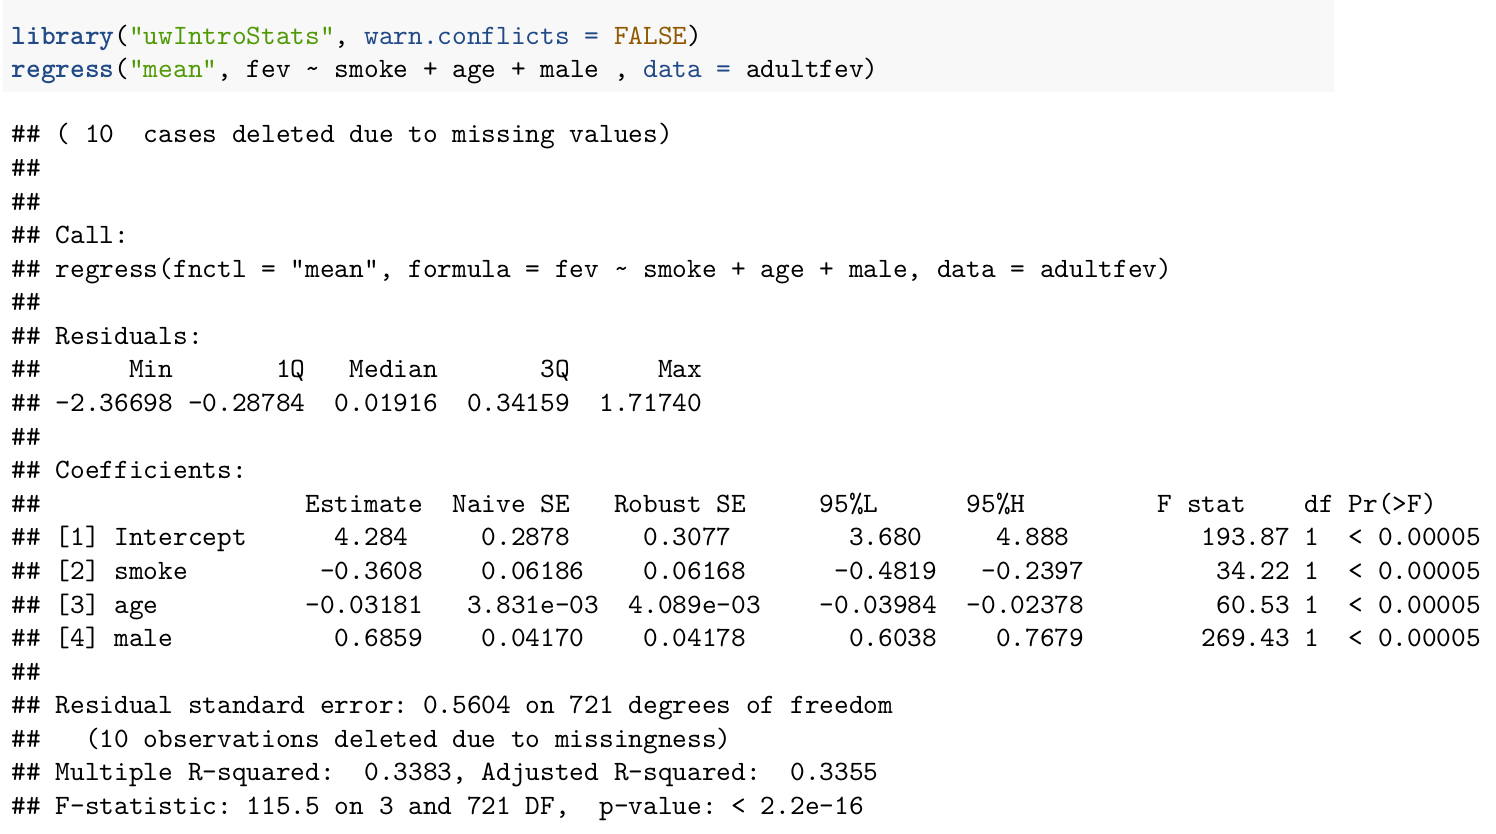
\includegraphics[width=1.1\textwidth]{plots/fev_vs_smoke_adjust_adultfev_noheight.png}
\end{center}
\end{frame}

\begin{frame}
\frametitle{Multiple linear regression: Adult FEV}
\vspace{-1cm}\textbf{Model:} {\small \begin{align*}
E(\text{FEV} \mid \text{Age}, \text{Male}, \text{Smoke}) =& \ \beta_0 + \beta_1 \text{Smoke} + \beta_2 \text{Age} + \beta_3 \text{Male} 
\end{align*} } \vspace{-1cm}

\textbf{Estimates:}
{\small \begin{align*}
\widehat{E}(\text{FEV} \mid \text{Age}, \text{Male}, \text{Smoke}) =& \ 4.28 + -0.36 (\text{Smoke}) \\
& -0.03 (\text{Age}) + 0.69 (\text{Male}) 
\end{align*} } \vspace{-1cm}

What is the interpretation of $\hat{\beta}_0 = 4.28$? \pause \textcolor{blue}{We estimate that among infant female nonsmokers, the mean FEV is $4.28$ L/second.} \textcolor{red}{Is this scientifically meaningful?}
\end{frame}

\begin{frame}
\frametitle{Multiple linear regression: Adult FEV}

What is the interpretation of $\hat{\beta}_1 = -0.36$? \pause \textcolor{blue}{We estimate that among two groups with the same sex and age, the average FEV among smokers is 0.36 L/second lower than among nonsmokers.}

Quantifying uncertainty? \pause \textcolor{blue}{Based on a 95\% confidence interval, this estimate would not be judged unusual if the true difference in mean FEV between smokers and nonsmokers of the same age and sex were between 0.48 and 0.24 L/second. This estimate is statistically significant at the 0.05 level ($p < 0.0001$).}

What is the scientific conclusion? \pause \textcolor{blue}{We have evidence to suggest that average FEV tends to be lower among smokers compared to nonsmokers, adjusting for age, and sex.}
\end{frame}

\begin{frame}
\frametitle{Multiple linear regression: Adult FEV}
\vspace{-0.5cm}\textbf{Model:} {\small \begin{align*}
E(\text{FEV} \mid \text{Age}, \text{Male}, \text{Smoke}) =& \ \beta_0 + \beta_1 \text{Smoke} + \beta_2 \text{Age} + \beta_3 \text{Male} 
\end{align*} } \vspace{-1cm}

What is the interpretation of $\hat{\beta}_2 = -0.03$? Should we report this $p$-value? \pause

\textcolor{blue}{$\hat{\beta}_2$: the estimated difference in mean FEV between two groups with the same smoking status and sex, but differing in age by 1 year, is 0.03 L/sec, with the older group having lower mean FEV.}

What is the interpretation of $\hat{\beta}_3 = 0.69$? \pause

\textcolor{blue}{$\hat{\beta}_3$: the estimated difference in mean FEV between males and females with the same smoking status and sex is 0.69 L/sec, with men tending to have higher FEV.}

\end{frame}

\begin{frame}
\frametitle{Multiple linear regression: precision variables}

Up to now, we have primarily been concerned with adjusting for \textcolor{red}{potential confounders}; if we fail to adjust for these variables, we may reach the wrong conclusion.

\textcolor{green}{Precision variables} (associated with the outcome in the population, not associated with the predictor of interest in the sample), in contrast, do not need to be adjusted for.

Adjusting for precision variables tends to \textcolor{green}{reduce the standard error for the coefficient of interest} (in linear regression): intuitively, we do a better job explaining the outcome, so we reduce the variability in the problem. 

Interpreting multiple linear regression coefficients \textcolor{blue}{is the same as if we adjusted for a confounder}.
\end{frame}

\begin{frame}
\frametitle{Multiple linear regression: precision variables}
\begin{center}
\vspace{-1cm}\hspace*{-0.5cm}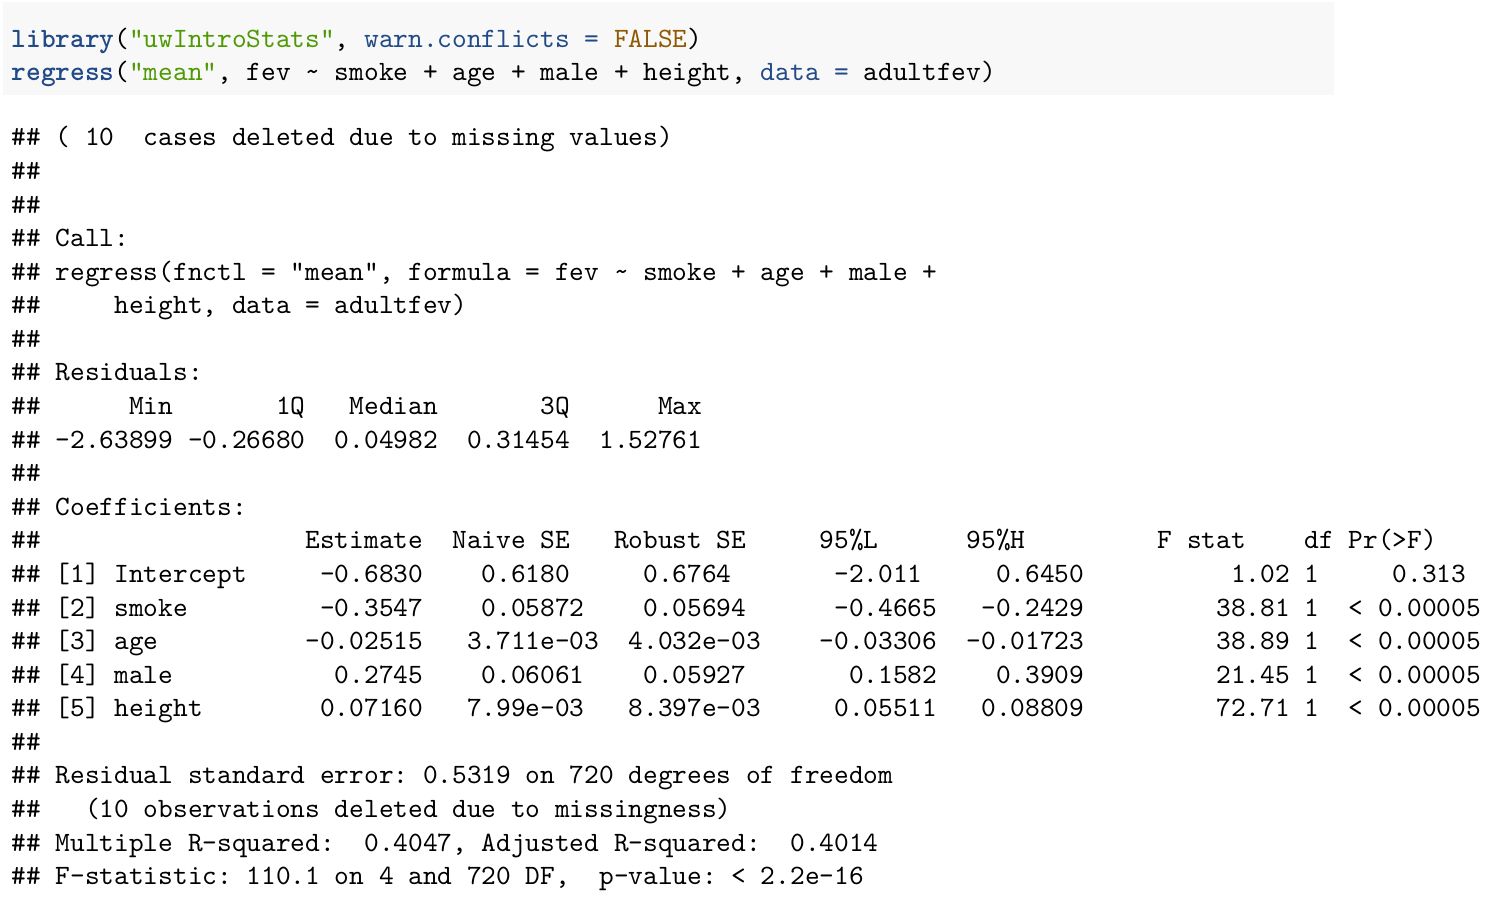
\includegraphics[width=1.1\textwidth]{plots/fev_vs_smoke_adjust_adultfev.png}
\end{center}

\end{frame}

\begin{frame}
\frametitle{Multiple linear regression: precision variables}
Table: Estimated difference in mean FEV comparing smokers to nonsmokers, not adjusted for height (Slide 1.122) and adjusted for height (Slide 1.127), along with robust standard errors and confidence intervals.

\hspace*{-1cm}\begin{tabular}{lccc}
\hline 
 & Estimate & Robust standard error & 95\% CI \\
 \hline 
No height & $-0.3608$ & $0.06168$  & [$-0.4819$, $-0.2397$]\\
Height & $-0.3547$ & $0.05694$ & [$-0.4665$, $-0.2429$]
\end{tabular}
\end{frame}

\begin{frame}
\frametitle{Multiple linear regression: effect modification}

With both \textcolor{red}{confounders} and \textcolor{green}{precision variables}, the association between the predictor of interest and the response \textbf{is the same} regardless of the value of the confounder/precision variable.

Sometimes, we have reason to believe that the association between our predictor of interest and the response \textcolor{blue}{differs depending on the value} of another variable.

We model this statistically by including an \textcolor{blue}{interaction} term between the predictor of interest and the potential effect modifier, \textbf{modeled as the multiplication of the two}.
\end{frame}

\begin{frame}
\frametitle{Multiple linear regression: effect modification}

If we are interested in the association between $X$ (POI) and $Y$ (outcome), \textcolor{blue}{but think that $Z$ is an effect modifier}, then we fit the regression model
\begin{align*}
E(Y \mid X, Z) = & \ \beta_0 + \beta_1 X + \beta_2 Z + \beta_3 (X \times Z).
\end{align*}

New terminology: the terms $X$ and $Z$ are the \textbf{main effects}, while the multiplicative term $(X \times Z)$ is called the \textbf{interaction} term.

\textcolor{red}{You may encounter situations where someone is looking for effect modification but does not include the main effects. \textbf{This can be misleading, so always include them.}}
\end{frame}

\begin{frame}
\frametitle{Multiple linear regression: effect modification}
For example, we might be interested in whether sex \textcolor{blue}{modifies the association} between smoking and FEV in older adults (65+). We use the regression model
\begin{align*}
E(\text{FEV} \mid \text{Smoker}, \text{Male}) = & \ \beta_0 + \beta_1 \text{Smoker} + \beta_2 \text{Male}\\
& + \beta_3 (\text{Smoker} \times \text{Male}).
\end{align*}

How do we interpret $\beta_0$? Is this scientifically sensible, and would you trust an estimate of it?\vspace{-0.2cm} \pause
\begin{itemize}
\item $\beta_0$: \textcolor{blue}{mean FEV among female nonsmokers} (i.e., Male = 0, Smoker = 0)
\item Reasonable to interpret (female nonsmokers exist)
\item Estimate is trustworthy (we measured females and nonsmokers)
\end{itemize}
\end{frame}

\begin{frame}
\frametitle{Multiple linear regression: effect modification}
\begin{align*}
E(\text{FEV} \mid \text{Smoker}, \text{Male}) = & \ \beta_0 + \beta_1 \text{Smoker} + \beta_2 \text{Male}\\
& + \beta_3 (\text{Smoker} \times \text{Male}).
\end{align*}

How do we interpret $\beta_1$? \pause
\textcolor{red}{We can't change Smoker but hold Smoker $\times$ Male constant, if Male = 1}: 
\begin{itemize}
\item if Smoker = 1 and Male = 1, Smoker $\times$ Male = 1
\item if Smoker = 0 and Male = 1, Smoker $\times$ Male = 0
\item $\beta_3$ \textcolor{red}{doesn't cancel out in our math game}
\end{itemize}
\end{frame}

\begin{frame}
\frametitle{Multiple linear regression: effect modification}
\begin{align*}
E(\text{FEV} \mid \text{Smoker}, \text{Male}) = & \ \beta_0 + \beta_1 \text{Smoker} + \beta_2 \text{Male}\\
& + \beta_3 (\text{Smoker} \times \text{Male}).
\end{align*}

Instead, to interpret $\beta_1$, we \textcolor{blue}{set Male = 0}:
{\small \begin{align*}
E(\text{FEV} \mid \text{Smoker} = 1, \text{Male} = 0) =&  \ \beta_0 + \beta_1 (1) + \beta_2 (0) + \beta_3 (1 \times 0) \\
= & \ \beta_0 + \beta_1 \\
E(\text{FEV} \mid \text{Smoker} = 0, \text{Male} = 0) =&  \ \beta_0 + \beta_1 (0) + \beta_2 (0) + \beta_3 (1 \times 0) \\
 =& \ \beta_0 \\
E(\text{FEV} \mid \text{Smoker} = 1, \text{Male} = 0) - \ &\\
E(\text{FEV} \mid \text{Smoker} = 0, \text{Male} = 0) =& \ \beta_1
\end{align*}
}
\end{frame}

\begin{frame}
\frametitle{Multiple linear regression: effect modification}
\begin{align*}
E(\text{FEV} \mid \text{Smoker}, \text{Male}) = & \ \beta_0 + \beta_1 \text{Smoker} + \beta_2 \text{Male}\\
& + \beta_3 (\text{Smoker} \times \text{Male}).
\end{align*}

$\beta_1$: \textcolor{blue}{the difference in mean FEV comparing \textbf{female smokers} to \textbf{female nonsmokers}.}
\begin{itemize}
\item Compare \textbf{across} levels of the variable whose coefficient we're interested in (here, smokers vs nonsmokers)
\item Compare \textbf{within} the group with value 0 for the effect modifier (here, Male = 0 means females)
\end{itemize}
\end{frame}

\begin{frame}
\frametitle{Multiple linear regression: effect modification}
\begin{align*}
E(\text{FEV} \mid \text{Smoker}, \text{Male}) = & \ \beta_0 + \beta_1 \text{Smoker} + \beta_2 \text{Male}\\
& + \beta_3 (\text{Smoker} \times \text{Male}).
\end{align*}

$\beta_2$: \textcolor{blue}{the difference in mean FEV comparing \textbf{male nonsmokers} to \textbf{female nonsmokers}.}
\begin{itemize}
\item Compare \textbf{across} levels of the variable whose coefficient we're interested in (here, males vs females)
\item Compare \textbf{within} the group with value 0 for the effect modifier (here, Smoker = 0 means nonsmokers)
\end{itemize}
\end{frame}

\begin{frame}
\frametitle{Multiple linear regression: effect modification}
\begin{align*}
E(\text{FEV} \mid \text{Smoker}, \text{Male}) = & \ \beta_0 + \beta_1 \text{Smoker} + \beta_2 \text{Male}\\
& + \beta_3 (\text{Smoker} \times \text{Male}).
\end{align*}

$\beta_3$: in our interpretation for the main effects and for confounders/precision variables, we have to \textcolor{red}{hold all other variables constant}, while changing the variable of interest.

But it is \textcolor{red}{impossible} to change Smoker $\times$ Male without changing either Smoker or Male!
\end{frame}

\begin{frame}
\frametitle{Multiple linear regression: effect modification}
\vspace{-0.7cm}
\begin{align*}
E(\text{FEV} \mid \text{Smoker}, \text{Male}) = & \ \beta_0 + \beta_1 \text{Smoker} + \beta_2 \text{Male}\\
& + \beta_3 (\text{Smoker} \times \text{Male}).
\end{align*}
\vspace{-0.3cm}
\textbf{When Male = 0:}  (i.e., among females) \vspace{-0.2cm}
\begin{itemize}
\item mean FEV among nonsmokers = $\beta_0 + \beta_2 \times 0 = \beta_0$; 
\item difference in mean FEV between smokers and nonsmokers = $\beta_1 + \beta_3 \times 0 = \color{blue}{\beta_1}$.
\end{itemize}

\textbf{When Male = 1:}  (i.e., among males) \vspace{-0.2cm}
\begin{itemize}
\item mean FEV among nonsmokers = $\beta_0 + \beta_2 \times 1 = \beta_0 + \beta_2$; 
\item difference in mean FEV between smokers and nonsmokers = $\beta_1 + \beta_3 \times 1 = \color{blue}{\beta_1 + \beta_3}$.
\end{itemize}

\textcolor{blue}{$\beta_3$: the difference in the difference in mean FEV between smokers and nonsmokers, comparing men and women.}
\end{frame}

\begin{frame}
\frametitle{Multiple linear regression: effect modification}
\vspace{-0.7cm}
\begin{align*}
E(\text{FEV} \mid \text{Smoker}, \text{Male}) = & \ \beta_0 + \beta_1 \text{Smoker} + \beta_2 \text{Male}\\
& + \beta_3 (\text{Smoker} \times \text{Male}).
\end{align*}
\vspace{-0.3cm}
\textbf{When Smoker = 0:}  (i.e., among nonsmokers) \vspace{-0.2cm}
\begin{itemize}
\item mean FEV among females = $\beta_0 + \beta_1 \times 0 = \beta_0$; 
\item difference in mean FEV between males and females = $\beta_2 + \beta_3 \times 0 = \color{blue}{\beta_2}$.
\end{itemize}

\textbf{When Smoker = 1:}  (i.e., among smokers) \vspace{-0.2cm}
\begin{itemize}
\item mean FEV among females = $\beta_0 + \beta_1 \times 1 = \beta_0 + \beta_1$; 
\item difference in mean FEV between males and females = $\beta_2 + \beta_3 \times 1 = \color{blue}{\beta_2 + \beta_3}$.
\end{itemize}

\textcolor{blue}{$\beta_3$: the difference in the difference in mean FEV between males and females, comparing smokers and nonsmokers.}
\end{frame}

\begin{frame}
\frametitle{Multiple linear regression: effect modification}
\begin{align*}
E(\text{FEV} \mid \text{Smoker}, \text{Male}) = & \ \beta_0 + \beta_1 \text{Smoker} + \beta_2 \text{Male}\\
& + \beta_3 (\text{Smoker} \times \text{Male}).
\end{align*}

The coefficient $\beta_3$ is a \textcolor{blue}{difference of differences}: we compare the difference in mean FEV between two groups, and compare that difference again.

We can also interpret $\beta_3$ as \textcolor{blue}{the difference between the sexes in the linear association of smoking and FEV.}

\end{frame}

\begin{frame}
\frametitle{Multiple linear regression: effect modification}
\vspace{-0.4cm}
\begin{align*}
E(Y \mid X, Z) =& \ \beta_0 + \beta_1 X + \beta_2 Z + \beta_3 (X \times Z)
\end{align*}
Interpreting the main effect of $X$ (e.g., smoking on mean FEV) in the presence of an interaction with $Z$ \textcolor{blue}{requires that Z} (e.g., male) \textcolor{blue}{equals zero.}

Interpretability now depends on: \vspace{-0.2cm}
\begin{itemize}
\item is $Z = 0$ scientifically meaningful? 
\item[] {\small (e.g., height = 0, SBP = 0 are implausible)}
\item is $Z = 0$ within the range of our data? 
\item[] {\small (e.g., age = 0 when our sample only contains age 65+)}
\end{itemize}

The multiplicative interaction $\beta_3 (X \times Z)$ means that effect modification is \textcolor{blue}{symmetric}: if Smoker modifies the association between Male and FEV, then Male also equally modifies the association between Smoker and FEV.
\end{frame}

\begin{frame}
\frametitle{Multiple linear regression: effect modification}
\begin{align*}
E(Y \mid X, Z) =& \ \beta_0 + \beta_1 X + \beta_2 Z + \beta_3 (X \times Z)
\end{align*}

If $\beta_3 = 0$, then the association between $X$ and $Y$ \textbf{is the same across strata} defined by $Z$---in other words, we have the same interpretation for $\beta_1$ as when we didn't include an interaction.

\textcolor{blue}{Testing whether $\beta_3 = 0$ directly tests effect modification.}

However, we \textcolor{red}{can't test the main effects of $X$ or $Z$ by themselves}---to test the overall association between, e.g., $X$ and $Y$, we must jointly test $\beta_1$ \textbf{and} $\beta_3$.

We won't cover how to do this in \texttt{R}, but it is possible.
\end{frame}

\begin{frame}
\frametitle{Multiple linear regression: effect modification}

To model effect modification in \texttt{R}, we use the same function as before, but with a slight tweak:
\begin{itemize}
\item \texttt{regress("mean", Y} $\sim$ \texttt{X + Z + X*Z)}, 
\item or equivalently, \texttt{regress("mean", Y} $\sim$ \texttt{X*Z)}
\item[] {\small \texttt{regress} includes the main effects by default }
\end{itemize}

Example: Adult FEV data, modeling effect modification of the smoking association with FEV by sex
\end{frame}

\begin{frame}
\frametitle{Multiple linear regression: effect modification}
\vspace{-1cm}\hspace*{-0.5cm}
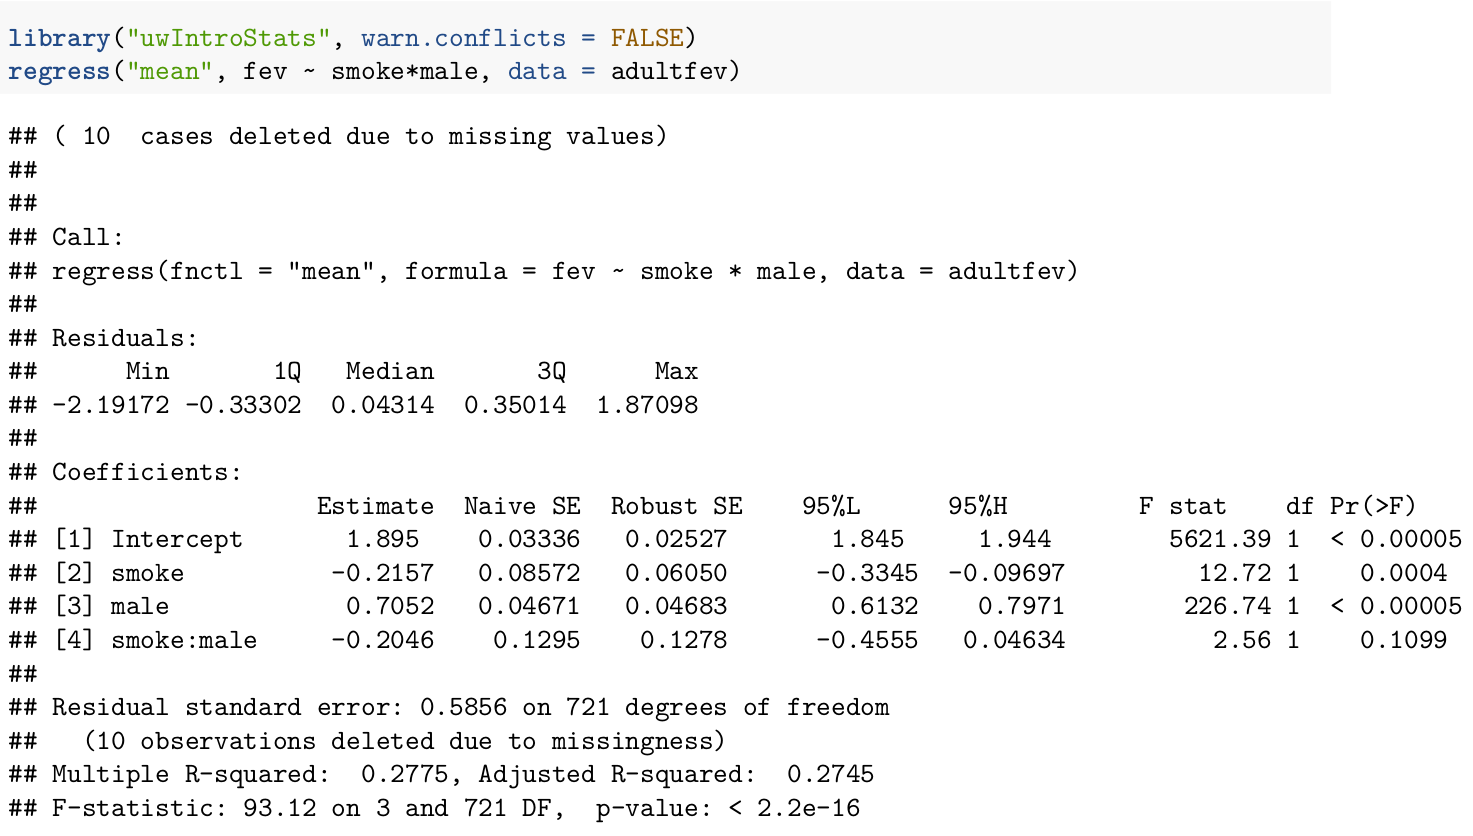
\includegraphics[width=1.1\textwidth]{plots/fev_smoke_sex_em.png}

\end{frame}

\begin{frame}
\frametitle{Multiple linear regression: effect modification}

The p-value for smoking on the previous slide was 0.0004. \textcolor{red}{Since we have an interaction term, we cannot use this p-value to test for an association between smoking and FEV}.

Typically, effect modification is a secondary scientific question: first, we want to know if smoking is associated with FEV at all; if it is, we might want to know \textcolor{blue}{if this association differs between the sexes}.

Thus, we can answer the two questions separately by fitting two separate regressions, one \textbf{without} the interaction term, and \textcolor{blue}{one \textbf{with} the interaction term}. 
\end{frame}


\begin{frame}
\frametitle{Multiple linear regression: effect modification}

Since both covariates (smoking, sex) were binary, we can actually calculate all within-group means from the estimated regression coefficients (this is called a \textcolor{blue}{saturated model}).

Stratified means from \texttt{descrip}: {\small \begin{tabular}{|c|c|c|}
\hline
 & Female & Male \\
 \hline
Nonsmoker & 1.90 & 2.60 \\
\hline
Smoker & 1.68 & 2.18  \\
\hline
\end{tabular}
}

Regression analysis results: 
\hspace*{-1cm}{\small \begin{tabular}{|c|c|c|}
\hline
 & Female & Male \\
 \hline
Nonsmoker & $\hat{\beta}_0$ & $\hat{\beta}_0 + \hat{\beta}_2$\\
& $ = 1.90$ &  $= 1.895 + 0.705 = 2.60$\\
\hline
Smoker & $\hat{\beta}_0 + \hat{\beta}_1$ & $\hat{\beta}_0 + \hat{\beta}_1 + \hat{\beta}_2 + \hat{\beta}_3$\\
& $ = 1.8895 - 0.216 = 1.68$ & $= 1.90 - 0.22 + 0.71 - 0.20 = 2.19$\\
\hline
\end{tabular}
}
\end{frame}

\begin{frame}
\frametitle{Multiple linear regression: effect modification}

\textcolor{blue}{We can model confounders and effect modifiers at the same time.} For example, in the adult FEV data, height is a potential confounder and sex may be an effect modifier:
\begin{align*}
E(\text{FEV} \mid \text{Smoker}, \text{Male}, \text{Height}) = & \ \beta_0 + \beta_1 \text{Smoker} + \beta_2 \text{Male}\\
& + \beta_3 (\text{Smoker} \times \text{Male}) + \beta_4 \text{Height}.
\end{align*}

Interpretation: 
\begin{itemize}
\item $\beta_0$: mean FEV among female nonsmokers with height 0''
\item $\beta_1$: difference in mean FEV comparing female smokers to female nonsmokers \textcolor{red}{of the same height}
\item $\beta_2$: difference in mean FEV comparing male nonsmokers to female nonsmokers \textcolor{red}{of the same height}
\end{itemize}
\end{frame}

\begin{frame}
\frametitle{Multiple linear regression: effect modification}

\textcolor{blue}{We can model confounders and effect modifiers at the same time.} For example, in the adult FEV data, height is a potential confounder and sex may be an effect modifier:
\begin{align*}
E(\text{FEV} \mid \text{Smoker}, \text{Male}, \text{Height}) = & \ \beta_0 + \beta_1 \text{Smoker} + \beta_2 \text{Male}\\
& + \beta_3 (\text{Smoker} \times \text{Male}) + \beta_4 \text{Height}.
\end{align*}

Interpretation: \vspace{-0.2cm}
\begin{itemize}
\item $\beta_3$: the difference between sexes in the linear association between smoking and FEV \textcolor{red}{for subjects of the same height}
\item[] the difference in the difference in mean FEV between smokers and nonsmokers, adjusted for height, between males and females
\item $\beta_4$: difference in mean FEV between two groups of the same sex and smoking status, but differing in height by one inch
\end{itemize}
\end{frame}

\begin{frame}
\frametitle{Multiple linear regression: effect modification}

If both variables involved in an interaction are binary, \textcolor{blue}{interpretation is fairly straightforward.}

We can fit the same type of regression model if one, or both, of the covariates are continuous---\textcolor{red}{all that changes is the scientific meaning of the regression parameters and trustworthiness of the estimated intercept and main effects.}

Example: Cognitive function and age

The Digit Symbol Substitution Test (DSST) measures cognitive function. We have data on 3775 participants, with an age range of 65--97 years. We are interested in the association between DSST (outcome) and age (POI), and possible effect modification by years of education. \textcolor{blue}{Regression model: 
\begin{align*}
E(\text{DSST} \mid \text{Age}, \text{Educ}) =& \ \beta_0 + \beta_1 \text{Age} + \beta_2 \text{Educ} + \beta_3 (\text{Age} \times \text{Educ})
\end{align*}
}
\end{frame}

\begin{frame}
\frametitle{Multiple linear regression: effect modification}

\vspace{-1cm}\hspace*{-0.5cm}
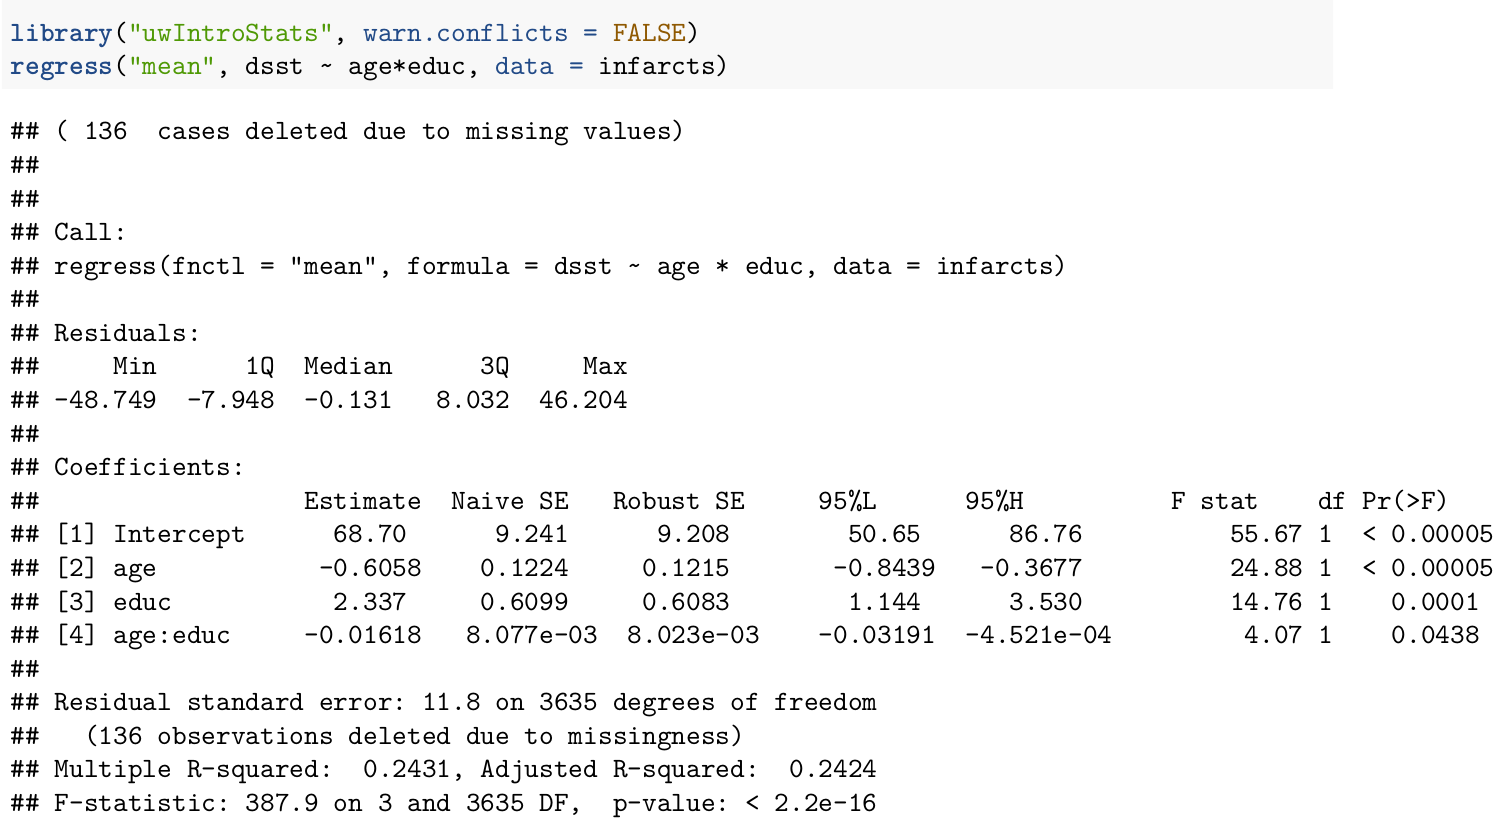
\includegraphics[width=1.1\textwidth]{plots/dsst_age_educ_em.png}

\end{frame}

\begin{frame}
\frametitle{Multiple linear regression: effect modification}
Coefficient interpretation:
\begin{itemize}
\item $\hat{\beta}_0$: estimated mean DSST score among those with age 0 and no education is 68.7 units
\item $\hat{\beta}_1$: estimated difference in mean DSST score between two groups differing in age by one year, both with no education is -0.61 units
\item $\hat{\beta}_2$: estimated difference in mean DSST score between two groups differing in education by one year, both with age 0 is 2.34 units
\end{itemize}

\textcolor{red}{Are any of these scientifically relevant?}
\end{frame}

\begin{frame}
\frametitle{Multiple linear regression: effect modification}
Coefficient interpretation:
\begin{itemize}
\item $\hat{\beta}_3$: We estimate that among individuals with one additional year of education, average DSST is lower by 0.02 units more per additional year of age than among individuals with one fewer year of education (95\% CI: [0.0005, 0.032]; p = 0.044)
\end{itemize}

This is a mouthful, but is correct. \textcolor{blue}{When in doubt, borrow this interpretation and replace with your variables}.

Here, we estimate that the association between older age and lower cognitive score is \textbf{larger} among people with more education---however, people with more education start off at a higher level of cognitive function. 
\end{frame}

\section{Prediction}
\begin{frame}
\frametitle{{\fontsize{15pt}{7.2}\selectfont SECTION 3: PREDICTION IN LINEAR REGRESSION}}

By the end of Section 3, you should be able to:
\begin{itemize}
\item Understand and explain the difference between the scientific goals of prediction versus causal association
\item[]
\item \textcolor{green}{Obtain predicted values from a linear regression analysis} by hand and using R
\item[]
\item Determine the \textcolor{blue}{predictive accuracy} of a linear regression analysis using $R^2$
\item[]
\item Understand and explain the \textcolor{magenta}{bias-variance tradeoff}
\end{itemize}
\end{frame}

\begin{frame}
\frametitle{Prediction versus (causal) association}
So far, in this course, our goal has been to estimate the association between a predictor of interest and our outcome.

Whether or not we need to adjust for other variables (\textcolor{red}{to deal with potential confounding}, \textcolor{green}{or increase precision}), or include interaction terms (\textcolor{blue}{for effect modification}) depends on the scientific question, which is aimed at these \textbf{associations}.

When our scientific question involves \textbf{prediction}, we have a different goal: \textcolor{magenta}{develop an algorithm based on current data that, when we plug in future data, predicts the outcome well.}
\end{frame}

\begin{frame}
\frametitle{Prediction: examples}
Some studies where prediction is the goal:
\begin{itemize}
\item \href{http://www.nature.com.offcampus.lib.washington.edu/articles/nature26000}{classifying tumors of the central nervous system} {\small (in Nature)}
\item \href{http://www.nejm.org.offcampus.lib.washington.edu/doi/full/10.1056/NEJMoa0804742}{predicting the risk of type II diabetes} {\small (in The New England Journal of Medicine)}
\item \href{https://www.ncbi.nlm.nih.gov/pubmed/28131393}{predicting immune response after completing an HIV vaccine trial} {\small (in Vaccine, by researchers at the Fred Hutchinson)}
\item predicting the sensitivity of HIV-1 viruses to neutralization by broadly neutralizing antibodies (my own research, paper to come soon!)
\end{itemize}
\end{frame}

\begin{frame}
\frametitle{Prediction: obtaining predictions}
Consider the linear regression model
\begin{align*}
E(Y \mid X_1, X_2, X_3) = & \ \beta_0 + \beta_1 X_1 + \beta_2 X_2 + \beta_3 X_3.
\end{align*}
I fit this linear regression, obtaining coefficient estimates; these are
\begin{align*}
\widehat{E}(Y \mid X_1, X_2, X_3) = & \ \hat{\beta}_0 + \hat{\beta}_1 X_1 + \hat{\beta}_2 X_2 + \hat{\beta}_3 X_3.
\end{align*}

Another name for $\widehat{E}(Y \mid X_1, X_2, X_3)$ is $\widehat{Y}$: these are the \textbf{fitted values}, obtained from drawing my best-fitting line through the data.

\textcolor{blue}{You have seen fitted values many times before:} for participants with all covariates equal to zero in your sample, the estimated intercept is the fitted value.

\end{frame}

\begin{frame}
\frametitle{Prediction: obtaining predictions}
There is \textbf{exactly one fitted value} corresponding to each participant in our data, and we call these $\widehat{Y}_i$, for $i = 1, 2, \dots, n$ (and $n$ is our sample size).

\textcolor{blue}{We obtain these fitted values simply by plugging in the covariates for the $i$th observation:}
\begin{align*}
\widehat{Y}_i = & \  \hat{\beta}_0 + \hat{\beta}_1 X_{i,1} + \hat{\beta}_2 X_{i,2} + \hat{\beta}_3 X_{i,3}.
\end{align*}

\textcolor{magenta}{In two dimensions, the line is our fitted values!} In higher dimensions, it is not quite as easy to conceptualize.
\end{frame}

\begin{frame}
\frametitle{Prediction: obtaining predictions}
\begin{center}
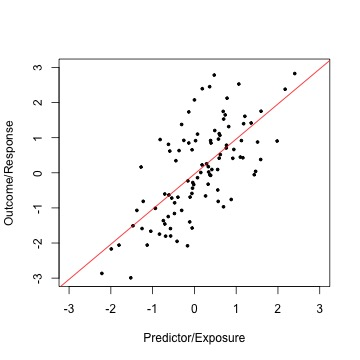
\includegraphics[width=0.7\textheight]{plots/linear-regr.jpg}
\end{center}
\end{frame}

\begin{frame}
\frametitle{Prediction: obtaining predictions}
Suppose you suddenly get data on the covariates of a \textcolor{magenta}{new participant}. 

\textcolor{red}{Without re-fitting your linear regression}, how might you obtain a predicted value based on this participant's covariates? \pause

Plug them in! 
\begin{align*}
\widehat{Y}_{n+1} = & \ \hat{\beta}_0 + \hat{\beta}_1 X_{(n+1),1} + \hat{\beta}_2 X_{(n+1),2} + \hat{\beta}_3 X_{(n+1),3}
\end{align*}

\textbf{In general, you can either do this by hand or use R to compute predicted values for you.}

Additionally, \textcolor{green}{the fitted values are our predictions of the mean outcome for the current study participants.}
\end{frame}

\begin{frame}
\frametitle{Prediction: extrapolation}
The intercept is the predicted mean value of the outcome for participants in our sample with all covariates equal to zero.

\textcolor{magenta}{If the assumption of linearity holds, then we might be okay extrapolating}... \textcolor{red}{but we have no way of knowing if it holds!}

We have already seen how extrapolating can provide reason not to report the estimated intercept in a linear regression.

\textcolor{red}{Using the linear regression formula to obtain predictions can create problems if we extrapolate far outside of our data for other predictions as well}: \vspace{-0.3cm}
\begin{itemize}
\item if my study only looks at tumors in the central nervous system, does it make sense to predict the type of a tumor found in the lymph nodes?
\item if I only consider people aged 65+, does it make sense to predict a health outcome for someone under 21?
\end{itemize}
\end{frame}

\begin{frame}
\frametitle{Prediction: Adult FEV}
The adult FEV dataset has 725 individuals, with measurements of age, FEV, height, sex, and smoking status.

On slide 1.147, we interpreted the coefficients in the linear regression model
\begin{align*}
E(\text{FEV} \mid \text{Smoker}, \text{Male}, \text{Height}) = & \ \beta_0 + \beta_1 \text{Smoker} + \beta_2 \text{Male} \\
&+ \beta_3 (\text{Smoker}\times\text{Male}) + \beta_4 \text{Height}.
\end{align*} 

Now we'll perform the regression, and extract \textbf{all coefficient estimates} to make predictions.
\end{frame}

\begin{frame}
\frametitle{Prediction: Adult FEV}
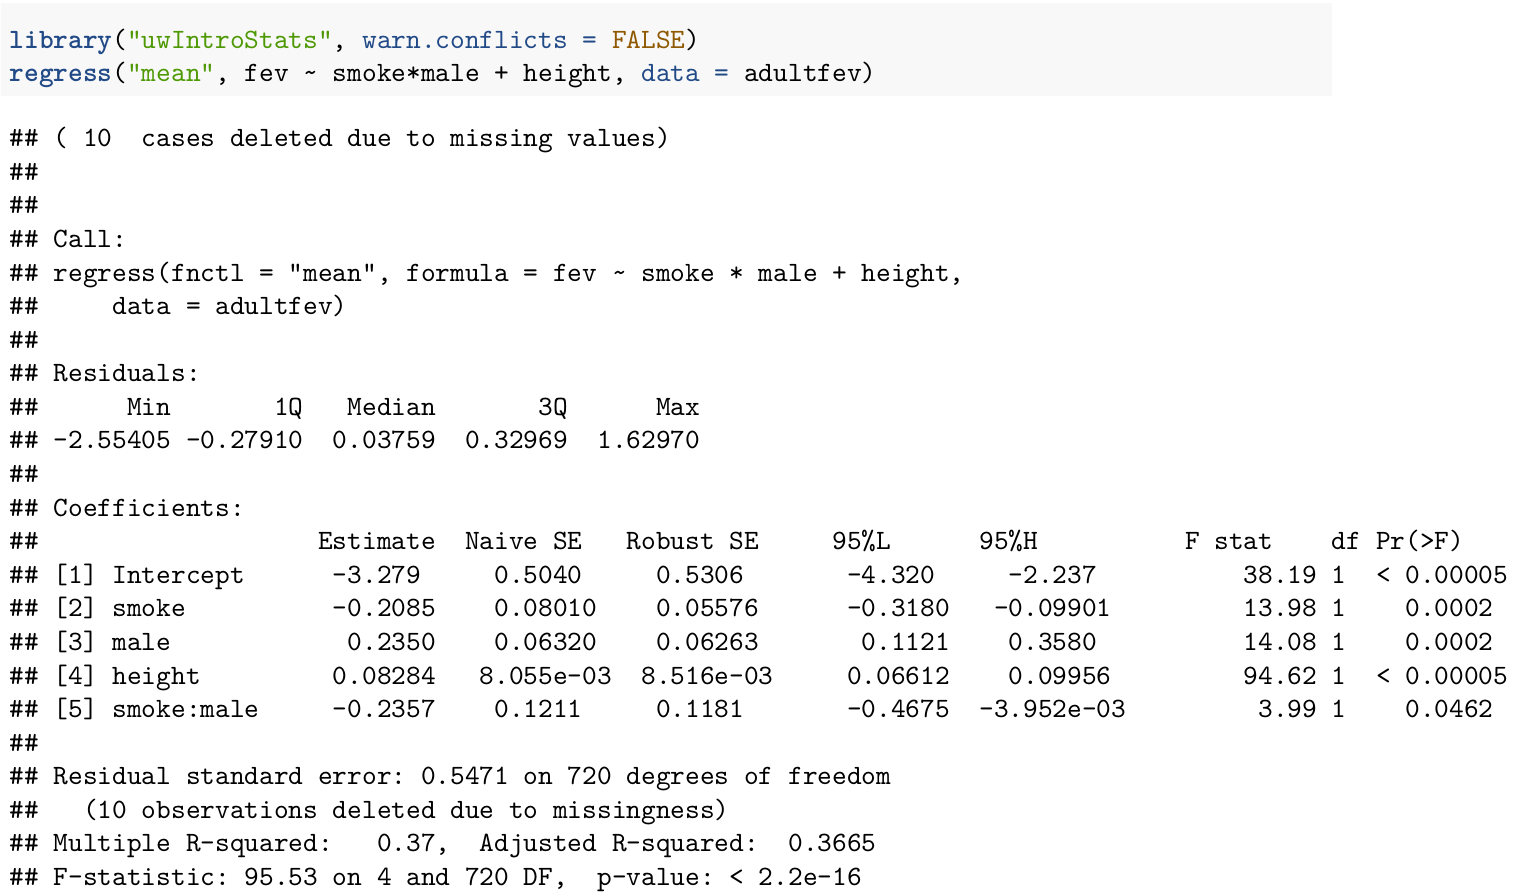
\includegraphics[width = 1.1\textwidth]{plots/predict_adult_fev.png}

\end{frame}

\begin{frame}
\frametitle{Prediction: Adult FEV}
\vspace{-0.5cm}
\begin{align*}
\widehat{Y} = & \ -3.28 - 0.21 \text{Smoker} + 0.24 \text{Male} + 0.08 \text{Height}\\
& - 0.24 (\text{Smoker}\times\text{Male}).
\end{align*}

What is our best estimate of the FEV for a \textcolor{blue}{nonsmoking} \textcolor{green}{female} who is \textcolor{magenta}{60 inches tall}? \pause
\begin{align*}
\widehat{Y} = & \ -3.28 - 0.21 \times 0 + 0.24 \times 0 + 0.08 \times 60 - 0.24 \times (0 \times 0) \\
=& \ -3.28 + 4.8 = 1.52
\end{align*} \pause

\vspace{-0.8cm}
What is our best estimate of the FEV for a \textcolor{blue}{smoking} \textcolor{green}{male} who is \textcolor{magenta}{72 inches tall}? \pause
\begin{align*}
\widehat{Y} = & \ -3.28 - 0.21 \times 1 + 0.24 \times 1 + 0.08 \times 72 - 0.24 \times (1 \times 1) \\
=& \ -3.28 -0.21 + 0.24 + 5.76 - 0.24 = 2.27
\end{align*} \pause

\vspace{-0.8cm}
\textcolor{blue}{Why ``best estimate''? Because these are our estimated mean $Y$ among people with $X_1 = x_1$, $X_2 = x_2$, etc.}
\end{frame}

\begin{frame}
\frametitle{Prediction: Adult FEV}
Use the \texttt{lm()} function to get predicted values in \texttt{R}:
\begin{center}
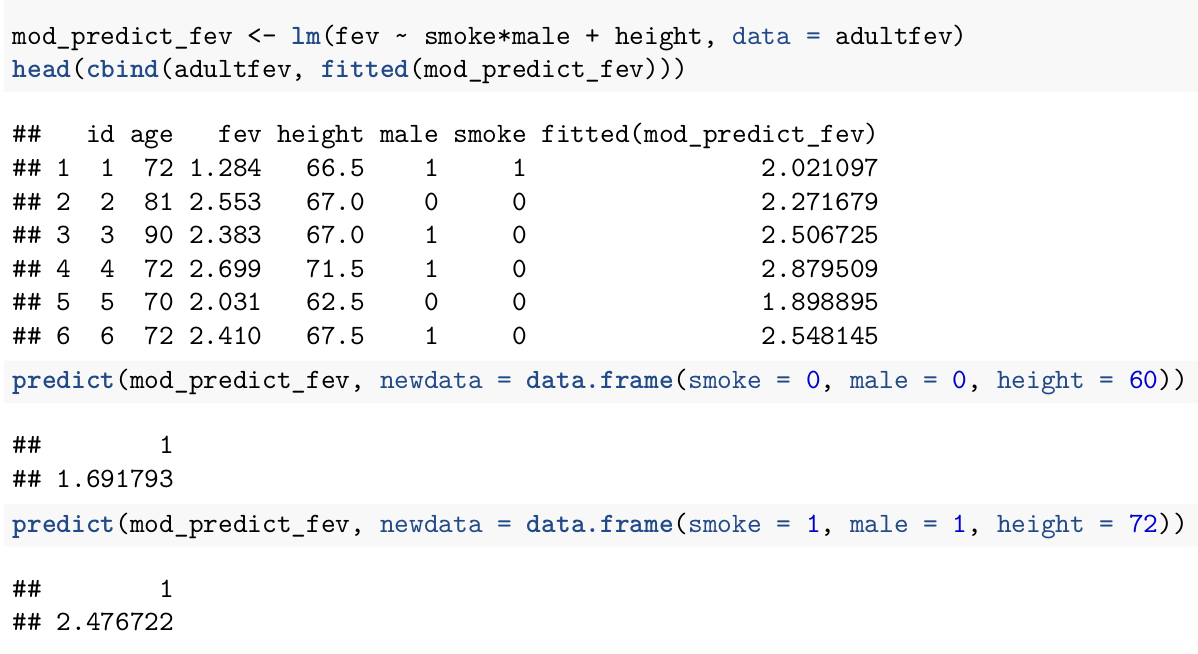
\includegraphics[width = 1\textwidth]{plots/predict_adult_fev_vals.png}
\end{center}
\end{frame}

\begin{frame}
\frametitle{Prediction: measuring accuracy}
\textcolor{magenta}{Goal of prediction: develop an algorithm based on current data that, when we plug in future data, predicts the outcome well.}

We typically measure ``well'' by thinking about the variance in the outcome explained by our predictive algorithm. 

The $R^2$ quantity makes this specific:
\begin{align*}
R^2 = & \ 1 - \frac{\text{squared difference between observations and fitted values}}{\text{variance of the outcome}} \\
= & \ 1 - \frac{\text{residual sum of squares (RSS)}}{\text{total sum of squares (TSS)}} \\
= & \ 1 - \frac{\sum_{i=1}^n (Y_i - \widehat{Y}_i)^2}{\sum_{i=1}^n (Y_i - \overline{Y}_i)^2} \\
=& \ \frac{\hat{\sigma}^2_Y - RSS/(n-1)}{\hat{\sigma}^2_Y}.
\end{align*}
\end{frame}

\begin{frame}
\frametitle{Prediction: measuring accuracy}
$R^2$ intuition:
\begin{itemize}
\item squaring differences makes above/below the line count equally
\item[]
\item residuals: difference between fitted line (fitted value) and response
\item[]
\item $R^2$ close to one: the ratio is close to zero, indicating that the difference between the observations and fitted values is much smaller than the variance
\item[]
\item $R^2$ close to zero: the ratio is close to 1, indicating that the fitted values are as good as using only the mean
\end{itemize}
\end{frame}

\begin{frame}
\frametitle{Prediction: measuring accuracy}
The regression output in \texttt{R} includes $R^2$ by default.

However, it actually displays two types:
\begin{itemize}
\item \texttt{Multiple R-squared} is the $R^2$ from slide 1.164--1.165
\item \texttt{Adjusted R-squared} is slightly different, and accounts for the number of model parameters
\end{itemize}

Finally, \texttt{R} estimates the standard error of the residuals, which is proportional to the square root of the RSS. 
\end{frame}

\begin{frame}
\frametitle{Prediction: Adult FEV}
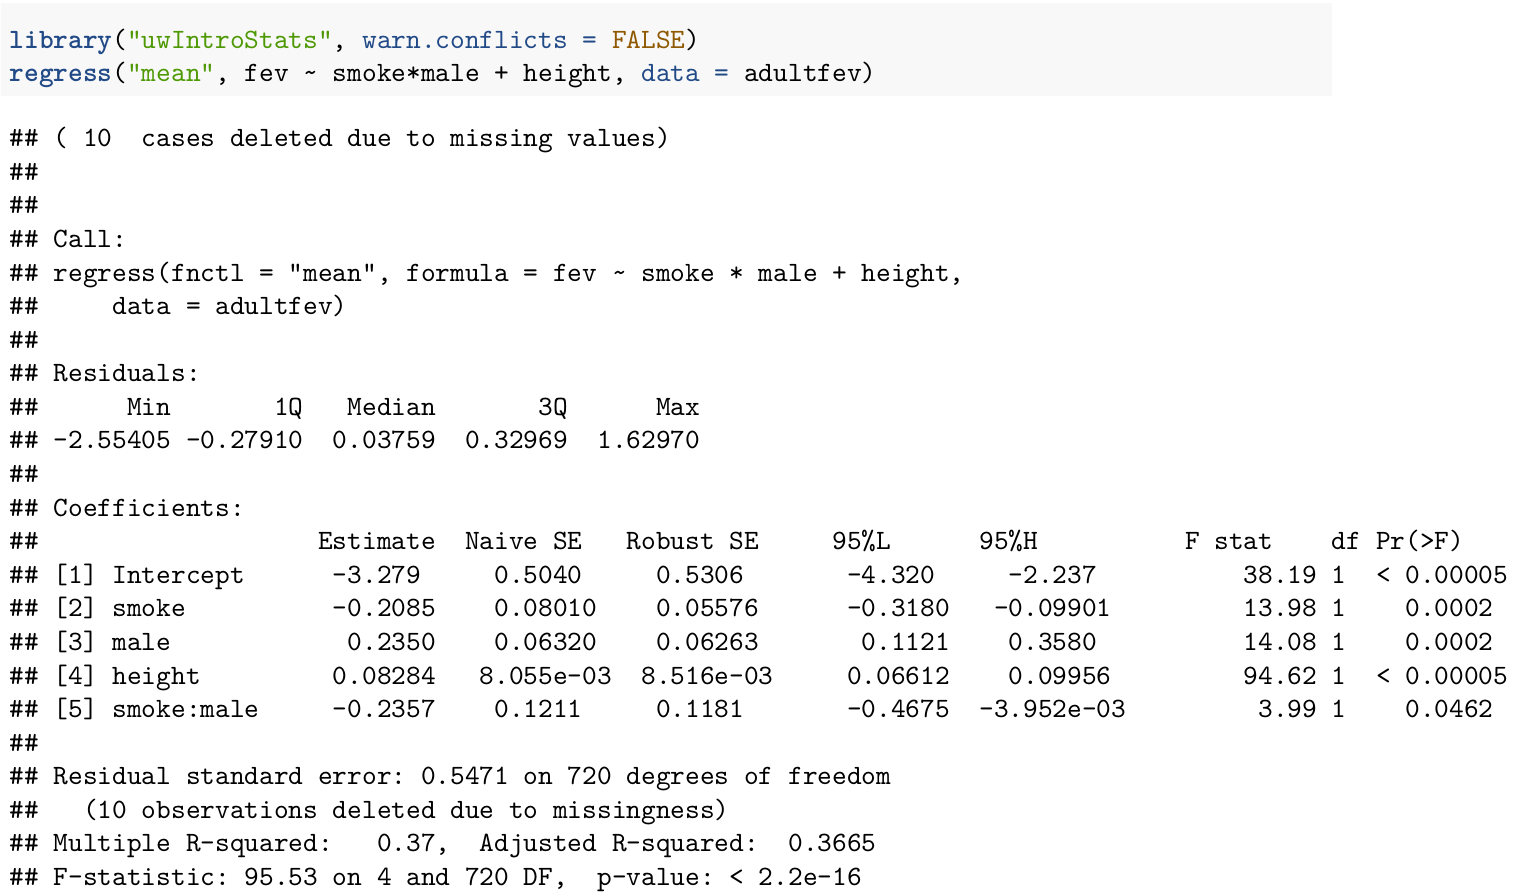
\includegraphics[width = 1.1\textwidth]{plots/predict_adult_fev.png}

\end{frame}

\begin{frame}
\frametitle{Prediction: bias-variance tradeoff}
Any estimation technique has $\begingroup\color{red}\text{bias}\endgroup$ and $\begingroup\color{Aquamarine}\text{variance}\endgroup$. 

These correspond to {\color{red}how far our estimates are from the truth} and {\color{Aquamarine}how variable our estimates are}.

In addition to $R^2$, we can measure prediction accuracy with $\begingroup\color{red}\text{bias}\endgroup^2 + \begingroup\color{Aquamarine}\text{variance}\endgroup $; this is called \textbf{mean squared error} (MSE), and is simply RSS/$n$.

Typically, inducing bias in our estimation will result in decreased variance, and vice versa.

\textbf{Least squares (fitting linear regression) finds the coefficients that minimize MSE! }(slides 1.32--1.35)
\begin{align*}
\hat{\beta} = & \ \argmin_\beta \frac{1}{n}\sum_{i=1}^n \{Y_i - (\beta_0 + \beta_1 X_{i,1} + \dots)\}^2
\end{align*}
\end{frame}

\begin{frame}
\frametitle{Prediction: bias-variance tradeoff}
Consider two options for obtaining predictions: we can either fit each point exactly (\emph{interpolating}), or fit linear regression. 

Interpolating has $\begingroup\color{red}\text{zero bias}\endgroup$ on the training data; linear regression has $\begingroup\color{red}\text{large bias}\endgroup$.

\centering
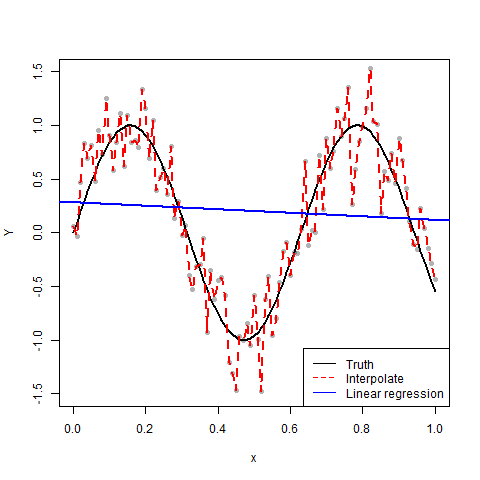
\includegraphics[width = 0.5\textwidth]{plots/bias_variance_tradeoff_1.png}
\end{frame}

\begin{frame}
\frametitle{Prediction: bias-variance tradeoff}
Moving one point from $(0.5, -0.58)$ to $(0.5, -0.08)$ changes the interpolating fit drastically, but doesn't change the linear regression fit. 

Interpolating has $\begingroup\color{Aquamarine}\text{large variance}\endgroup$; linear regression has $\begingroup\color{Aquamarine}\text{small variance}\endgroup$.
 
\centering
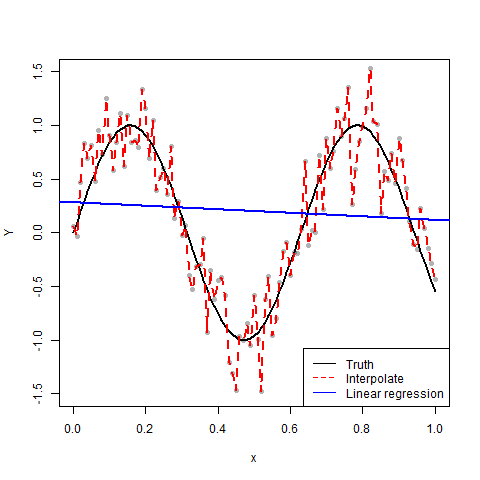
\includegraphics[width = 0.5\textwidth]{plots/bias_variance_tradeoff_1.png}
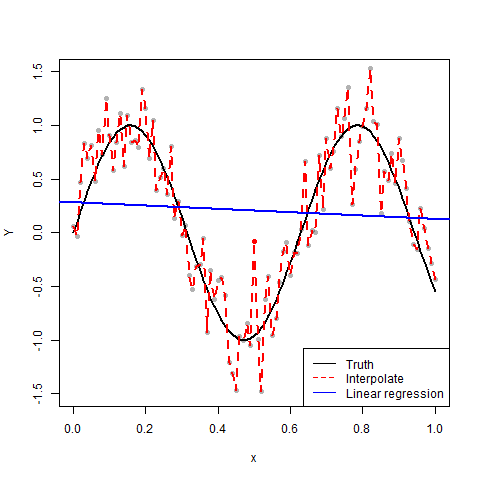
\includegraphics[width = 0.5\textwidth]{plots/bias_variance_tradeoff_2.png}
\end{frame}

\begin{frame}
\frametitle{Prediction: summary}
If our scientific goal is to obtain predictions, then we have different concerns than when we are interested in associations: \vspace{-0.3cm}
\begin{itemize}
\item \textcolor{red}{extrapolating is more dangerous}
\item we have to balance the bias and variance of our estimators
\item we want ``good'' predictions ($R^2$ near 1, MSE low)
\end{itemize}

We can get actual values of predictions by either: \vspace{-0.3cm}
\begin{itemize}
\item reading off regression coefficients and plugging in new values by hand, or
\item using the \texttt{lm()} and \texttt{predict()} functions in \texttt{R}
\end{itemize}

Making good predictions is a hot topic in statistics currently, and \textcolor{green}{``machine learning'' methods are often the best predictive algorithms}; however, \textcolor{blue}{in many settings linear regression can be used to predict well, and is often more interpretable than ``black box'' methods.}
\end{frame}

\section{Wrapping up}
\begin{frame}
\frametitle{SECTION 4: SUMMARY}

We have spent a lot of time interpreting linear regression coefficients, confidence intervals, and p-values.

Depending on your scientific question and your study design, you may need to adjust for \textcolor{red}{potential confounders} and/or \textcolor{green}{precision variables}, and you may include interaction terms to test \textcolor{blue}{effect modification}.

We have also spent considerable time honing your data analysis workflow.
\end{frame}

\begin{frame}
\frametitle{SECTION 4: SUMMARY}
Data analysis workflow: \vspace{-0.3cm}
\begin{itemize}
\item Write a \textcolor{blue}{scientific question}
\item[]
\item Draw a \textcolor{green}{causal diagram}
\item[]
\item Write a \textcolor{orange}{statistical question that uses the causal diagram and answers the scientific question}
\item[]
\item \textcolor{magenta}{Fit linear regression in R}:
\begin{itemize}
\item compute descriptive statistics and graphics in support of a linear regression analysis
\item perform linear regression
\end{itemize}
\end{itemize}
\end{frame}

\begin{frame}
\frametitle{SECTION 4: SUMMARY}
Data analysis workflow (continued): \vspace{-0.3cm}
\begin{itemize}
\item Interpret results:
\begin{itemize}
\item \textcolor{cyan}{interpretation of regression coefficients}
\item is the interpretation \textcolor{violet}{scientifically meaningful}?
\item will the estimate of the coefficient \textcolor{red}{rely on extrapolation}?
\item decide whether or not to report an estimate based on scientific meaning and lack of extrapolation
\end{itemize}
\item[]
\item Report results:
\begin{itemize}
\item \textbf{4 numbers}: estimate (units!), CI (units!), p-value (round if smaller than $0.001$)
\item \textbf{5 parts}: interpret each number, \textbf{add a sentence answering the scientific question}
\end{itemize}
\end{itemize}
\end{frame}

\begin{frame}
\frametitle{Linear regression: inflammatory biomarkers}
The Cardiovascular Health Study is a government sponsored cohort study of adults aged 65 years and older in four communities.

The primary goals of the study were to, over an 11 year period:\vspace{-0.3cm}
\begin{itemize}
\item observe the incidence of cardiovascular disease (especially heart attacks and congestive heart failure)
\item observe the incidence of cerebrovascular disease (especially strokes) in the elderly 
\item relate the incidence of those diseases to various risk factors measured in the population on a regular basis
\end{itemize}
\end{frame}

\begin{frame}
\frametitle{Linear regression: inflammatory biomarkers}
In this study, over 5,000 elderly, generally healthy (cancer was an exclusion criterion), adults were randomly selected from Medicare rolls in four communities.

For this analysis, we are interested in the role of inflammation in the pathogenesis of atherosclerotic disease. \textbf{In particular, we are interested in two biochemical markers of inflammation, the C reactive protein and fibrinogen.}

We have the following information on each subject: age (years), sex (\texttt{male}: male = 1, female = 0), cholesterol (\texttt{cholest}, mg/dL), BMI (\texttt{bmi}, kg/m${}^2$), previous history of cardiovascular disease (\texttt{prevdis}: 1/0), fibrinogen (\texttt{fib}, mg/dL), and C reactive protein (\texttt{crp}, mg/L).
\end{frame}

\begin{frame}
\frametitle{Linear regression: inflammatory biomarkers}
\textbf{Our scientific question:} are \textcolor{orange}{blood levels of fibrinogen} associated with \textcolor{blue}{blood levels of C reactive protein}? \pause

\textcolor{green}{Causal diagram: } {\small (space intentionally left blank)} \vspace{5cm}

\end{frame}

\begin{frame}
\frametitle{Linear regression: inflammatory biomarkers}
\textbf{Our scientific question:} are \textcolor{orange}{blood levels of fibrinogen} associated with \textcolor{blue}{blood levels of C reactive protein}?

\textbf{Our statistical question:} is there a \textcolor{orange}{difference in mean blood fibrinogen level} \textcolor{blue}{comparing two groups with a one mg/L difference in blood levels of C reactive protein among older adults of the same age, sex, cholesterol, BMI, and with the same previous history of cardiovascular disease}?

Now that we have a rigorous statistical question, we can fit a linear regression in \texttt{R}. The linear model implied by this question is
\begin{align*}
E(\text{Fib} \mid & \text{CRP}, \text{Age}, \text{Male}, \text{Cholest.}, \text{BMI}, \text{Prev. Hist.}) =  \ \beta_0 + \beta_1 \text{CRP} \\
&+ \beta_2 \text{Age}  + \beta_3 \text{Male} + \beta_4 \text{Cholest.} + \beta_5 \text{BMI} + \beta_6 \text{Prev. Hist.}
\end{align*}
\end{frame}

\begin{frame}
\frametitle{Linear regression: inflammatory biomarkers}
{\small 
\begin{align*}
E(\text{Fib} \mid & \text{CRP}, \text{Age}, \text{Male}, \text{Cholest.}, \text{BMI}, \text{Prev. Hist.}) =  \ \beta_0 + \beta_1 \text{CRP} \\
&+ \beta_2 \text{Age}  + \beta_3 \text{Male} + \beta_4 \text{Cholest.} + \beta_5 \text{BMI} + \beta_6 \text{Prev. Hist.}
\end{align*}
}
Is the regression parameter \textcolor{magenta}{scientifically meaningful}? \vspace{-0.3cm}
\begin{itemize}
\item $\beta_0$: \pause \textcolor{red}{no; age 0, BMI 0, cholesterol 0 don't make sense}
\item $\beta_1$: \pause \textcolor{blue}{yes, parameter of interest!}
\item $\beta_2$: \pause yes (but not meaningful for \textbf{this} scientific question) (why?)
\item $\beta_3$: yes (but not meaningful for \textbf{this} scientific question)
\item $\beta_4$: yes (but not meaningful for \textbf{this} scientific question)
\item $\beta_5$: yes (but not meaningful for \textbf{this} scientific question)
\item $\beta_6$: yes (but not meaningful for \textbf{this} scientific question)
\end{itemize} 

\end{frame}

\begin{frame}
\frametitle{Linear regression: inflammatory biomarkers}
{\small 
\begin{align*}
E(\text{Fib} \mid & \text{CRP}, \text{Age}, \text{Male}, \text{Cholest.}, \text{BMI}, \text{Prev. Hist.}) =  \ \beta_0 + \beta_1 \text{CRP} \\
&+ \beta_2 \text{Age}  + \beta_3 \text{Male} + \beta_4 \text{Cholest.} + \beta_5 \text{BMI} + \beta_6 \text{Prev. Hist.}
\end{align*}
}
Will our estimate \textcolor{red}{rely on extrapolation}? \vspace{-0.3cm}
\begin{itemize}
\item $\beta_0$: \pause yes, don't observe anyone age 0, cholesterol 0, BMI 0
\item $\beta_1$: \pause no
\item $\beta_2$: no
\item $\beta_3$: no
\item $\beta_4$: no
\item $\beta_5$: no
\item $\beta_6$: no
\end{itemize} 

\end{frame}

\begin{frame}
\frametitle{Linear regression: inflammatory biomarkers}
{\small 
\begin{align*}
E(\text{Fib} \mid & \text{CRP}, \text{Age}, \text{Male}, \text{Cholest.}, \text{BMI}, \text{Prev. Hist.}) =  \ \beta_0 + \beta_1 \text{CRP} \\
&+ \beta_2 \text{Age}  + \beta_3 \text{Male} + \beta_4 \text{Cholest.} + \beta_5 \text{BMI} + \beta_6 \text{Prev. Hist.}
\end{align*}
}
Which estimates should we report?
\begin{itemize}
\item $\beta_0$: \pause no
\item $\beta_1$: \textcolor{blue}{yes (predictor of interest!!)}
\item $\beta_2$: \pause no
\item $\beta_3$: no
\item $\beta_4$: no
\item $\beta_5$: no
\item $\beta_6$: no
\end{itemize}
\end{frame}

\begin{frame}
\frametitle{Linear regression: inflammatory biomarkers}
\hspace*{-0.5cm}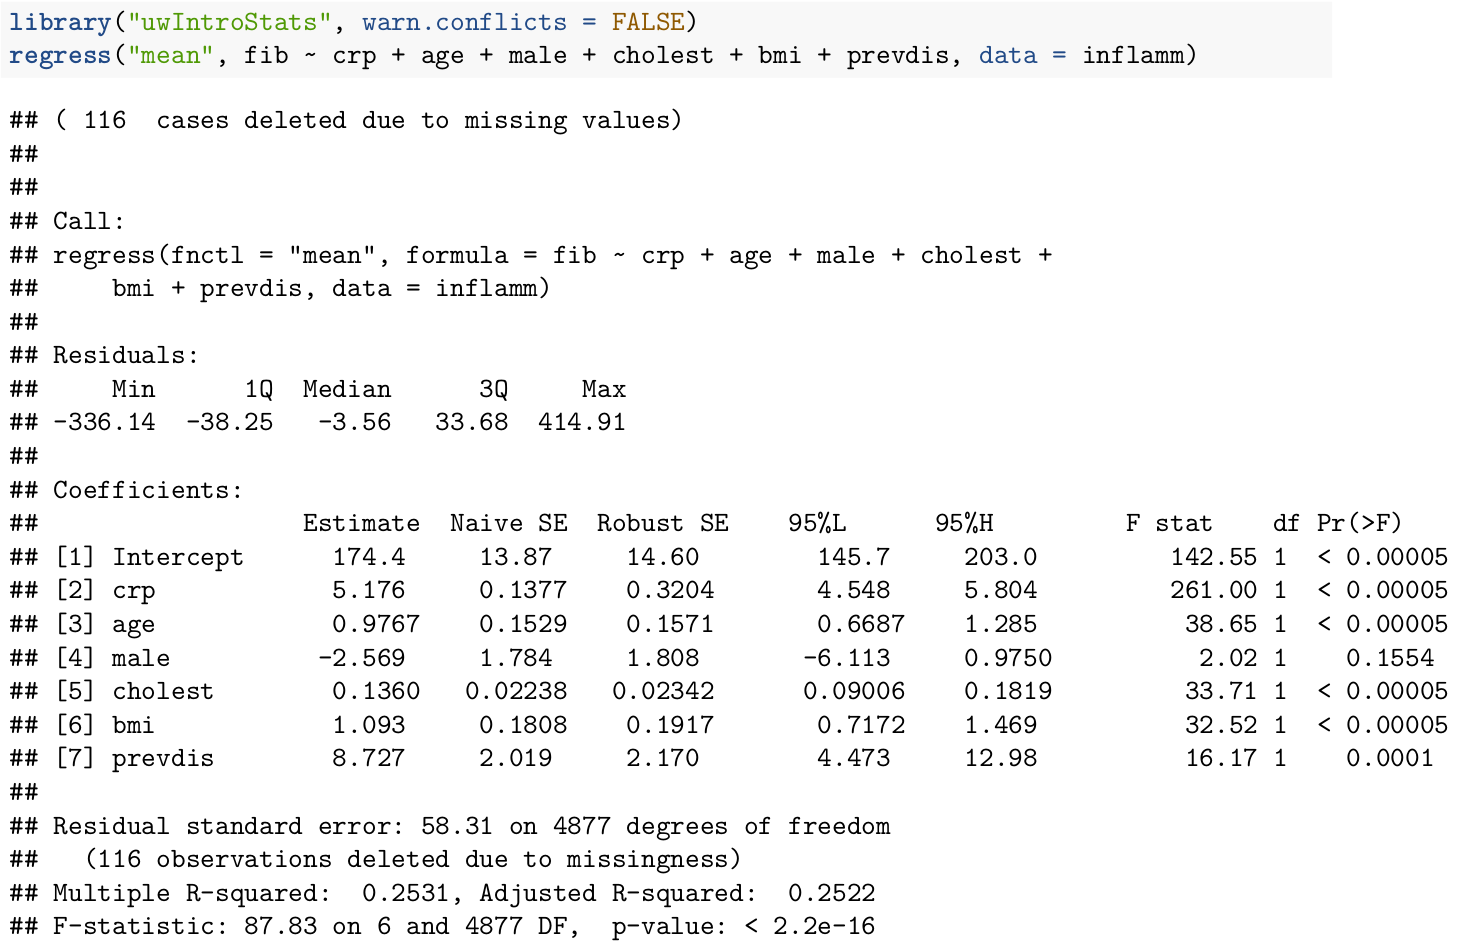
\includegraphics[width = 1.1\textwidth]{plots/inflamm_fib_vs_crp.png}
\end{frame}

\begin{frame}
\frametitle{Linear regression: inflammatory biomarkers}\textcolor{cyan}{Interpretation of $\hat{\beta}_1$:} 

The \textcolor{orange}{estimated difference in mean blood fibrinogen level} between \textcolor{blue}{two groups differing in blood C reactive protein level by one mg/L}, but \textcolor{red}{with the same age, sex, blood cholesterol level, BMI, and previous history of cardiovascular disease}, is \textcolor{magenta}{5.18 mg/dL}, where the group with the higher blood level of C reactive protein tends to have the higher blood level of fibrinogen.
\end{frame}

\begin{frame}
\frametitle{Linear regression: inflammatory biomarkers}

\textbf{Summary of results:} \textit{(part 1, interpretation)}

Based on a linear regression, we estimate that the \textcolor{orange}{mean difference in mean blood fibrinogen level} between \textcolor{blue}{two groups differing in blood C reactive protein level by one mg/L}, but \textcolor{red}{with the same age, sex, blood cholesterol level, BMI, and previous history of cardiovascular disease}, is \textcolor{magenta}{5.18 mg/dL}, where the group with the higher blood level of C reactive protein tends to have the higher blood level of fibrinogen. 
\end{frame}

\begin{frame}
\frametitle{Linear regression: inflammatory biomarkers}

\textbf{Summary of results:} \textit{(part 2, statistical inference)}

\textcolor{green}{Based on a 95\% confidence interval, this result would not be judged unusual if the true difference in mean blood fibrinogen level were between 4.55 and 5.80 mg/dL} comparing two groups differing in blood C reactive protein level by one mg/L, but having the same age, sex, cholesterol level, BMI, and previous history of cardiovascular disease. \textcolor{orange}{This result is statistically significant (p-value $< 0.001$)}. \textcolor{blue}{Based on these results, we have evidence to suggest that blood levels of C reactive protein are associated with blood levels of fibrinogen, adjusted for age, sex, cholesterol, BMI, and previous history of cardiovascular disease.}
\end{frame}

\begin{frame}
\frametitle{Linear regression: inflammatory biomarkers}
\textbf{New scientific question:} does \textcolor{orange}{the association between C reactive protein and fibrinogen} \textcolor{blue}{differ based on age}? 

\textbf{Statistical question:} \textcolor{blue}{is there a difference} in \textcolor{orange}{the difference in mean blood fibrinogen level comparing two groups with a one mg/L difference in blood levels of C reactive protein among older adults with the same sex, cholesterol, BMI, and previous history of cardiovascular disease}, \textcolor{blue}{comparing two groups differing in age by one year}?

This statistical question implies the linear regression model
{\small 
\begin{align*}
E(\text{Fib} \mid & \text{CRP}, \text{Age}, \text{Male}, \text{Cholest.}, \text{BMI}, \text{Prev. Hist.}) =  \ \beta_0 + \beta_1 \text{CRP} \\
&+ \beta_2 \text{Age}  + \beta_3 \text{Male} + \beta_4 \text{Cholest.} + \beta_5 \text{BMI} + \beta_6 \text{Prev. Hist.} \\
&+ \beta_7 (\text{CRP} \times \text{Age}),
\end{align*}
}
and the hypothesis test of interest is
\begin{align*}
H_0: \beta_7 = &\ 0 \\
H_a: \beta_7 \neq &\ 0.
\end{align*}
\end{frame}


\end{document}
